\documentclass{zkdl-presentation-template}

% -- Auxiliary Packages --
\usepackage{pgffor}
\usepackage{bbm}

% -- Algorithms --
\usepackage[
    titlenumbered,
    linesnumbered,
    ruled
]{algorithm2e}
\SetKwInOut{Input}{Input}
\SetKwInOut{Output}{Output}
\SetKwInOut{Return}{Return}

% --- Ticks and crosses ---
\usepackage{pifont} % http://ctan.org/pkg/pifont
\newcommand{\cmark}{\textcolor{green!65!black}{\ding{51}}}%
\newcommand{\xmark}{\textcolor{red!80!black}{\ding{55}}}%

% --- Tikz ---
\usetikzlibrary{tikzmark, backgrounds, shapes.geometric, arrows.meta, positioning, fit}

% --- Title Page Info ---
\title[Bionetta]{Bionetta: Ultimate ZKML Framework}
\author{Distributed Lab \\ Rarimo}
\date{April 25, 2025}
\homepage{distributedlab.com/}
\github{rarimo/bionetta-tf}

\begin{document}
    \frame {
        \tikz [remember picture,overlay]
        \node at
            ([yshift=3.0cm,xshift=-3.0cm]current page.south east) 
            %or: (current page.center)
            {
\includegraphics[width=100pt]{logo.png}};
        \titlepage
    }

	\section{Intro to ZKML}

    \begin{frame}{What is a neural network?}
        \only<1>{
            \begin{center}
                \large Think of a \textcolor{gray!80!black}{neural network} as a
                \textbf{black box}\ldots
            \end{center}
    
            \vspace{10px}
    
            \begin{figure}
                \centering
                
\includegraphics[width=0.5\textwidth]{images/nn_1.pdf}
            \end{figure}
        }
        \only<2>{
            \begin{center}
                \large This \textbf{black box} takes some input
                $\textcolor{green!60!black}{\boldsymbol{x}}$ (e.g., image or a text
                prompt)\ldots
            \end{center}
            
            \vspace{10px}

            \begin{figure}
                \centering
                
\includegraphics[width=0.6\textwidth]{images/nn_2.pdf}
            \end{figure}
        }
        \only<3>{
            \begin{center}
                \large Besides the \textcolor{green!60!black}{input
                $\boldsymbol{x}$}, you can tweak the parameters
                \textcolor{blue}{$\theta$} of the black box --- so-called
                \textcolor{blue}{\textit{weights}} --- which changes the behavior of
                the black box. They are typically \textit{fixed}\ldots
            \end{center}
            \vspace{10px}
            \begin{figure}
                \centering
                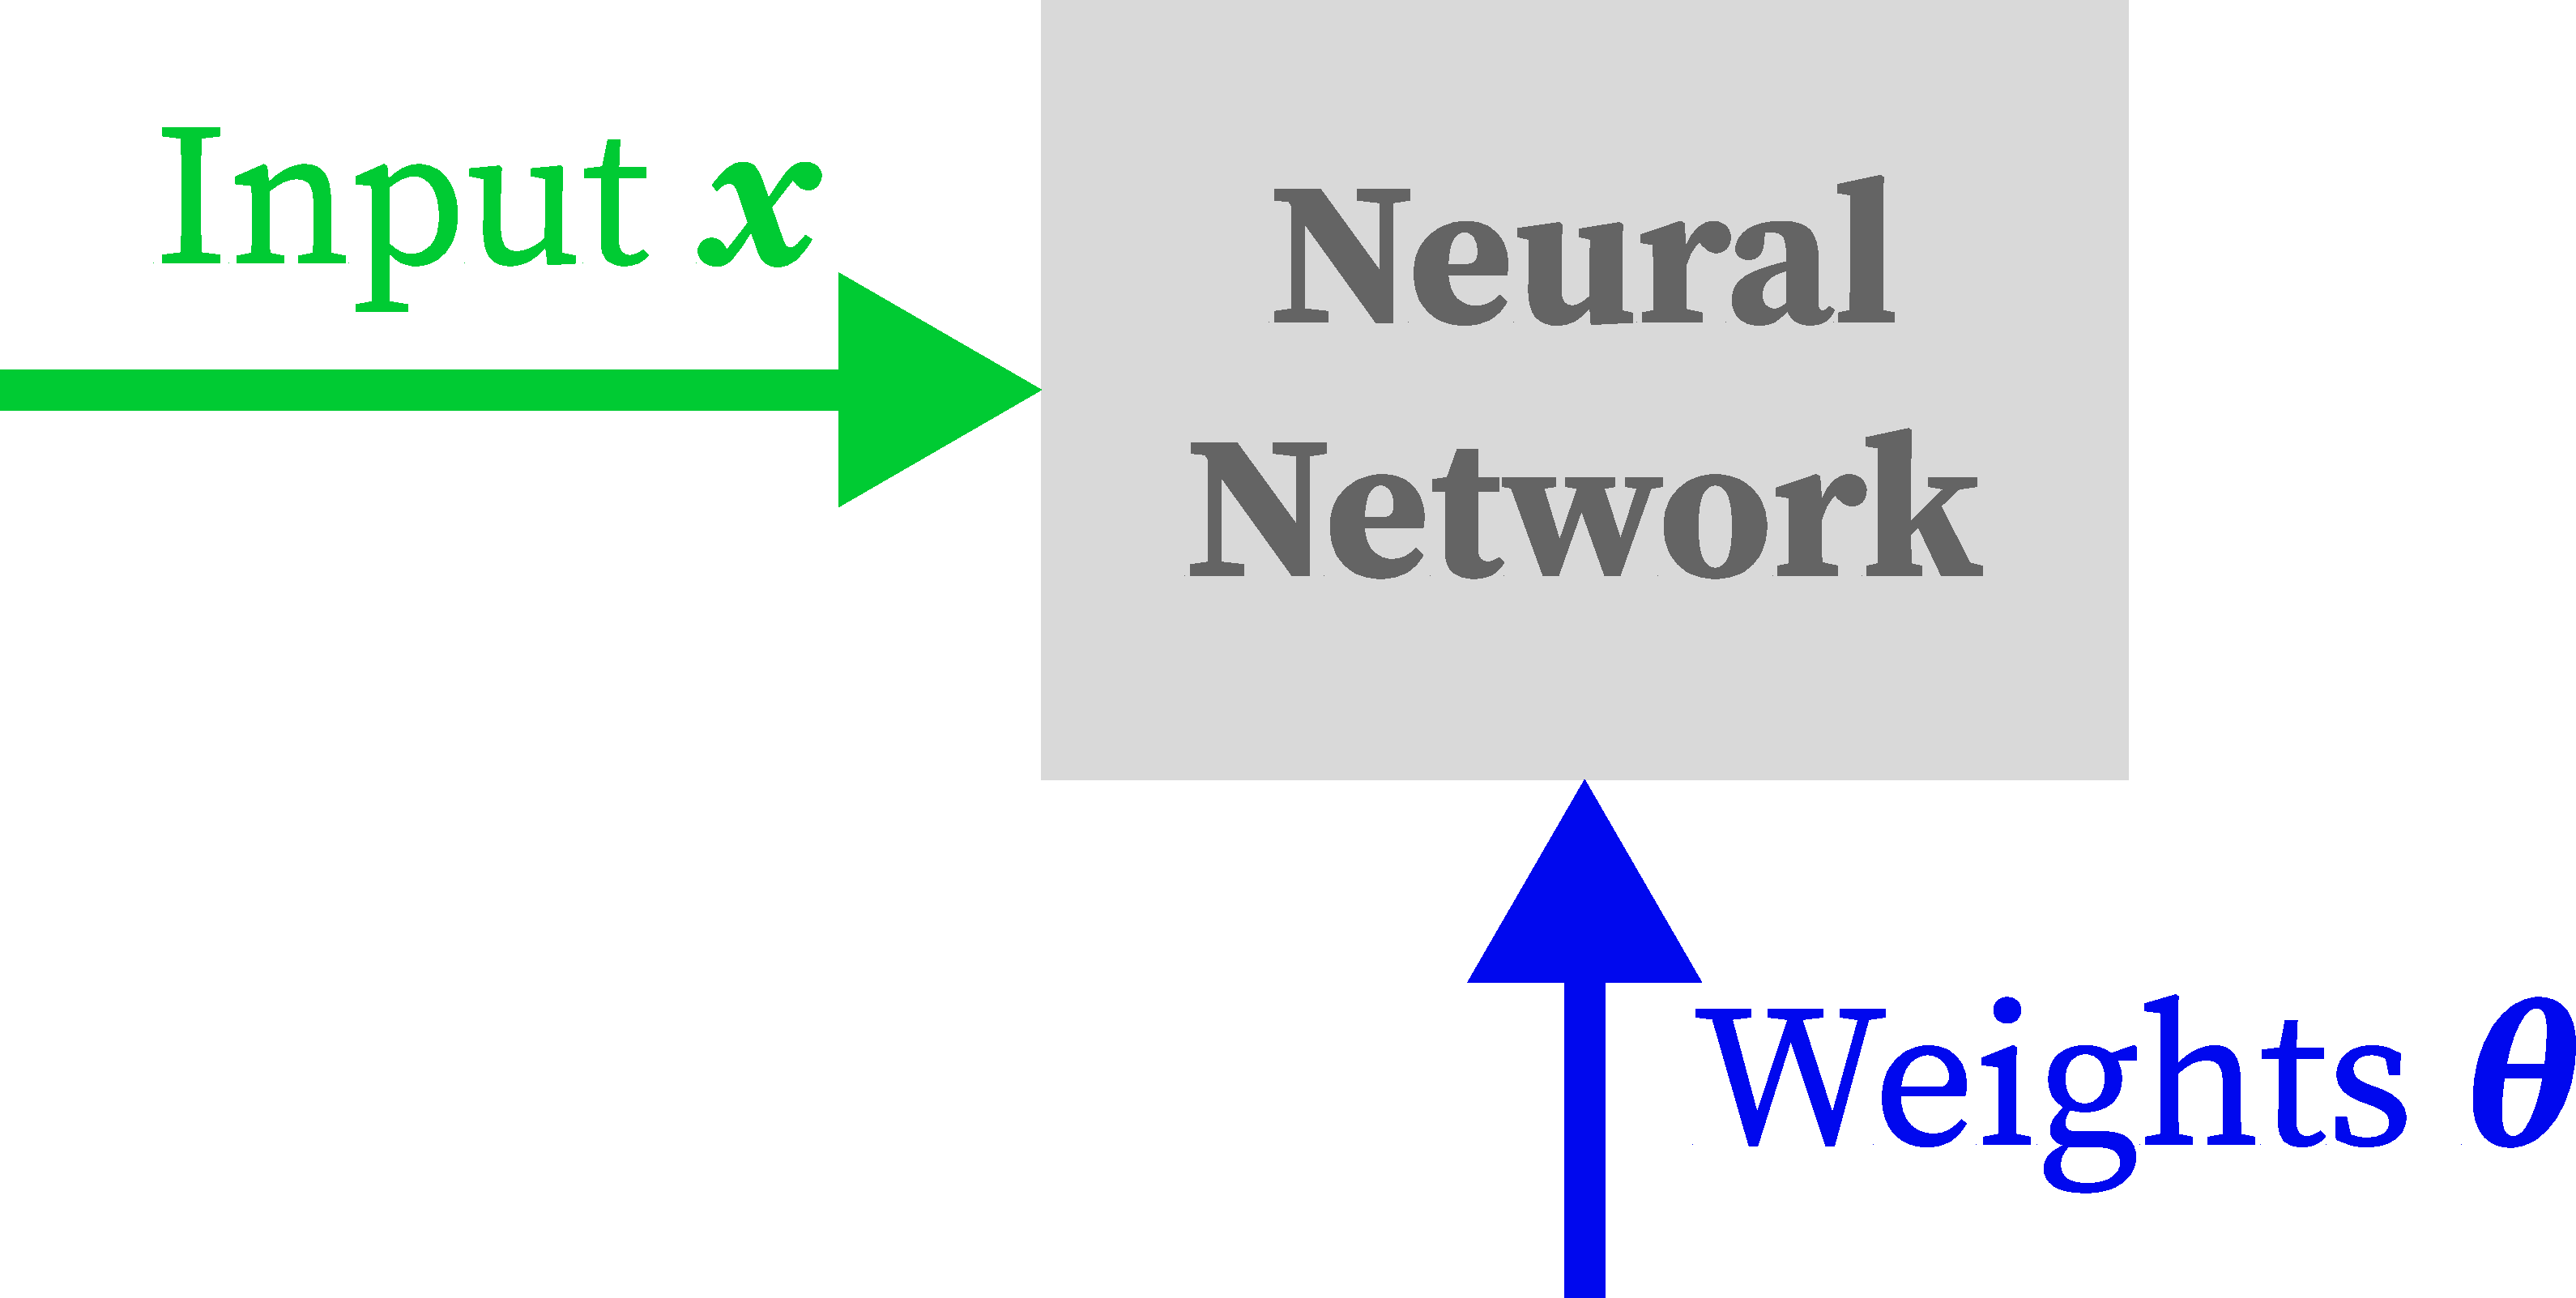
\includegraphics[width=0.7\textwidth]{images/nn_3.pdf}
            \end{figure}
        }
        \only<4-5>{
            \begin{center}
                \large Given the \textcolor{green!60!black}{inputs $\boldsymbol{x}$}
                and \textcolor{blue}{weights $\boldsymbol{\theta}$}, you can get the
                \textcolor{purple}{prediction $\boldsymbol{y}$} (e.g., person's features or 
                AI's text response)\ldots
            \end{center}
    
            \vspace{10px}
    
            \begin{figure}
                \centering
                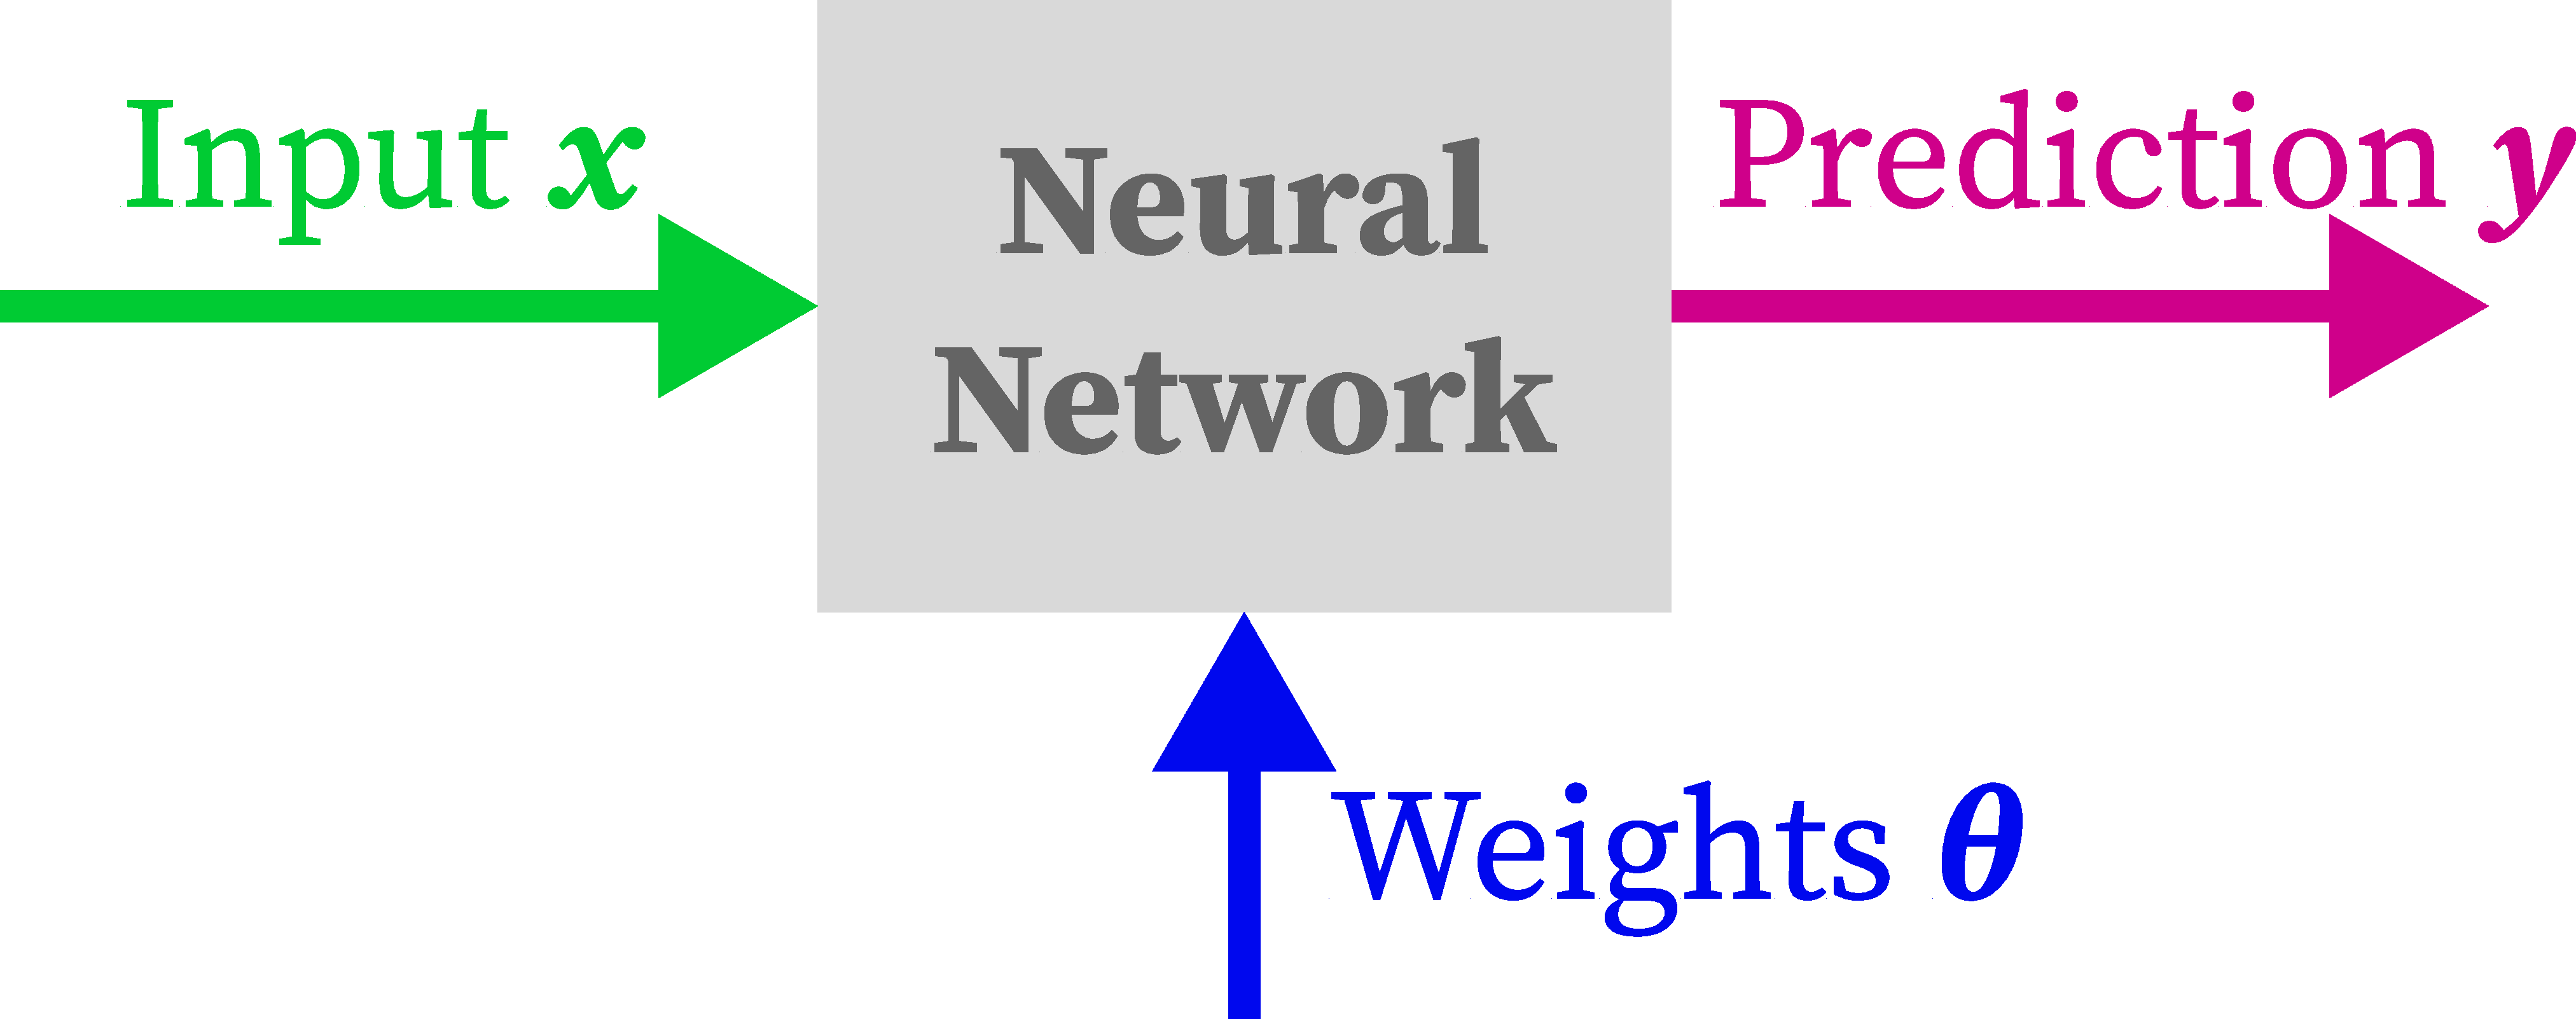
\includegraphics[width=0.8\textwidth]{images/nn_4.pdf}
            \end{figure}
        }
        \only<5>{
            \vspace{10px}
        
            \begin{center}
                \large We denote such computation as $\textcolor{purple}{\boldsymbol{y}} = \textcolor{gray!80!black}{f}(\textcolor{green!60!black}{\boldsymbol{x}};\textcolor{blue}{\boldsymbol{\theta}})$.
            \end{center}
        }
        \only<6>{
            Though, in practice everything is \textit{quite complicated}\ldots
            \begin{figure}
                \centering
                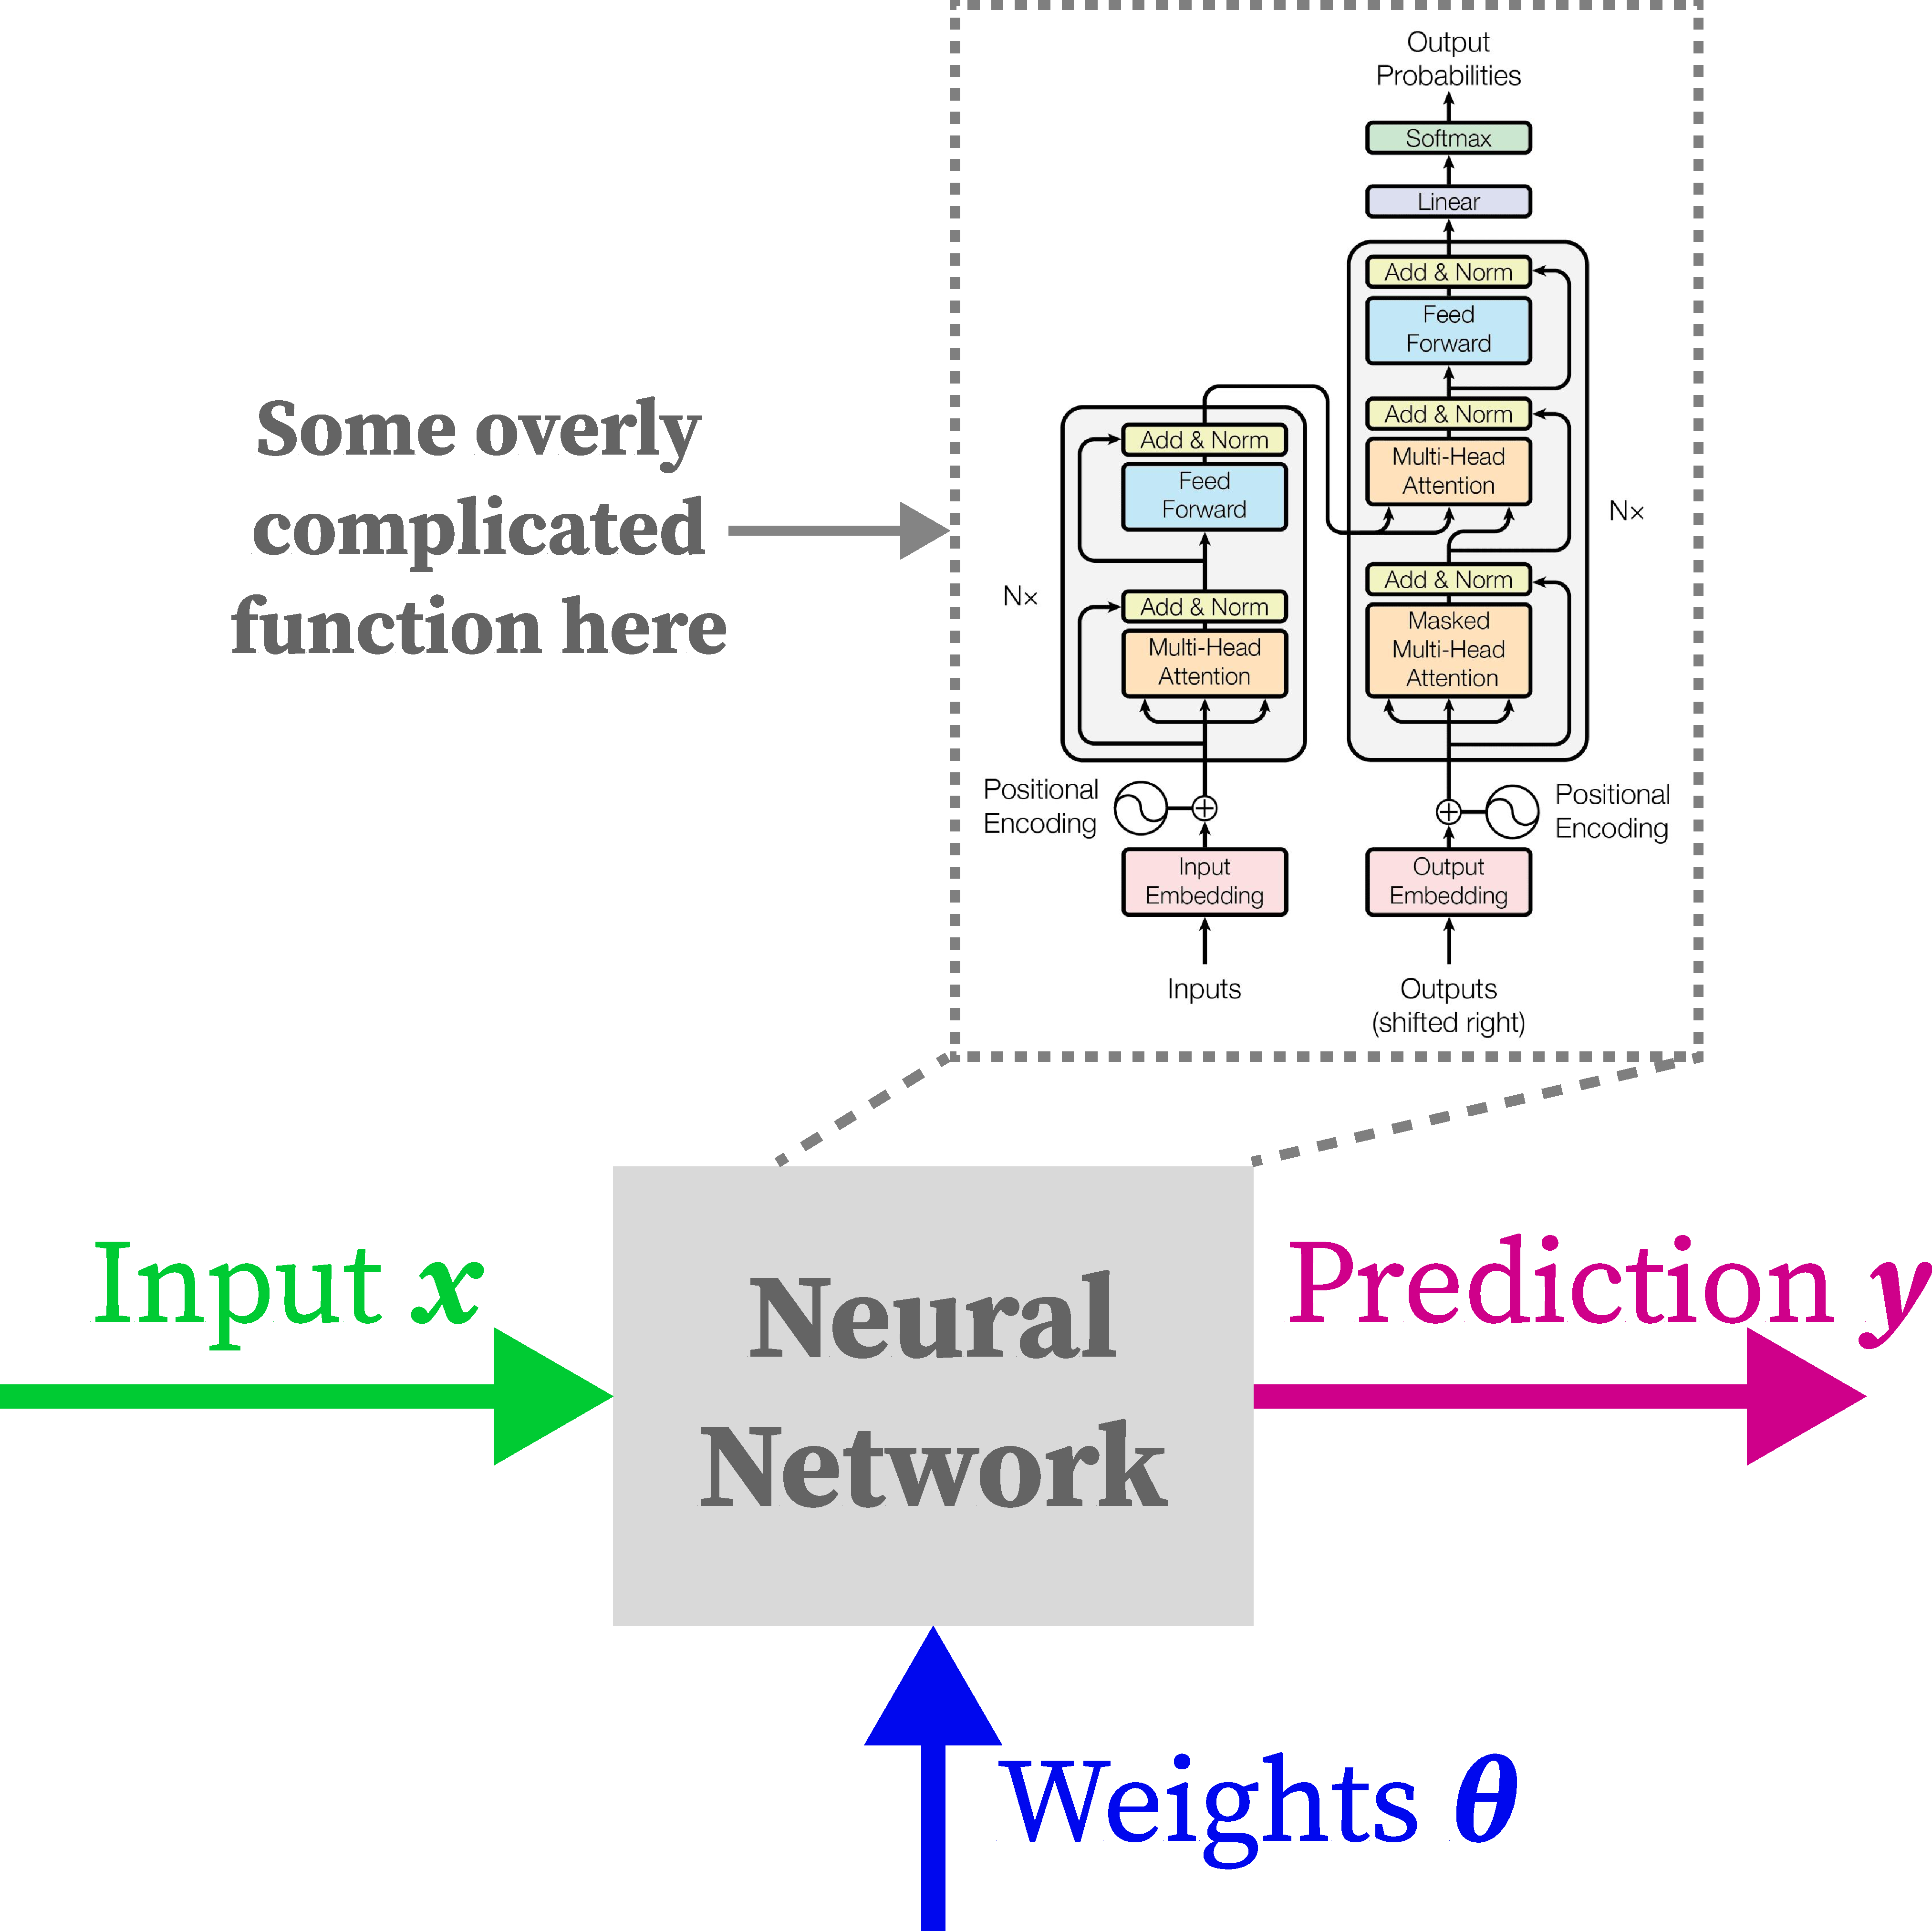
\includegraphics[width=0.65\textwidth]{images/nn_5.pdf}
            \end{figure}
        }
    \end{frame}

    \begin{frame}{Where ZK?}
        \begin{center}
            So why do we need ZK in this process?
        \end{center}
        \begin{figure}
            \centering
            
\includegraphics[width=0.85\textwidth]{images/where.pdf}
        \end{figure}
    \end{frame}

    \begin{frame}{ZKML: Engineering Perspective}
        \only<1>{
            \begin{figure}
                \centering
                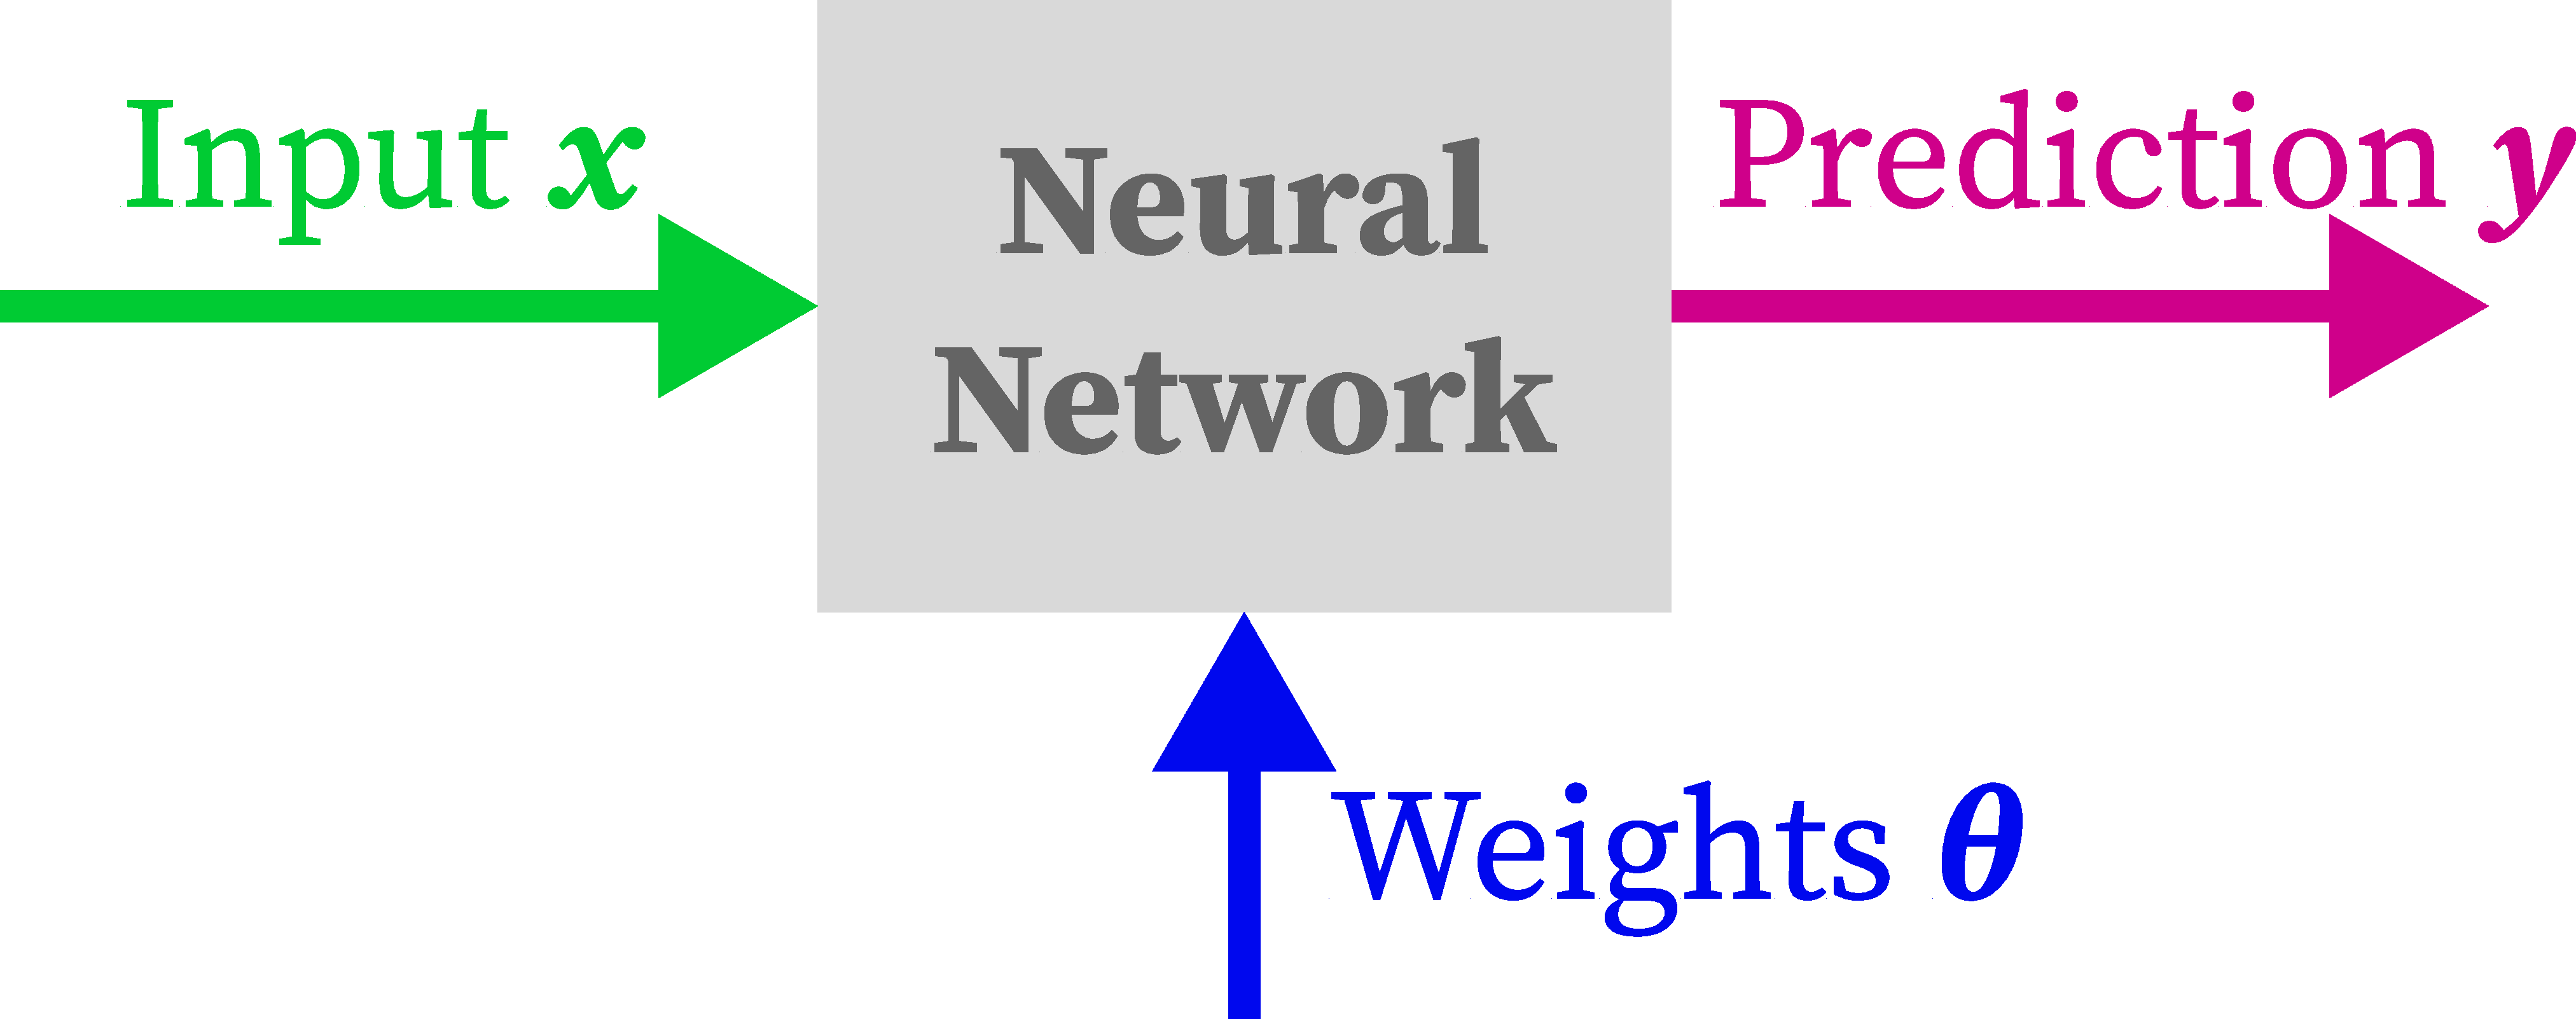
\includegraphics[width=0.75\textwidth]{images/nn_4.pdf}
            \end{figure}
        }
        \only<2-3>{
            \begin{figure}
                \centering
                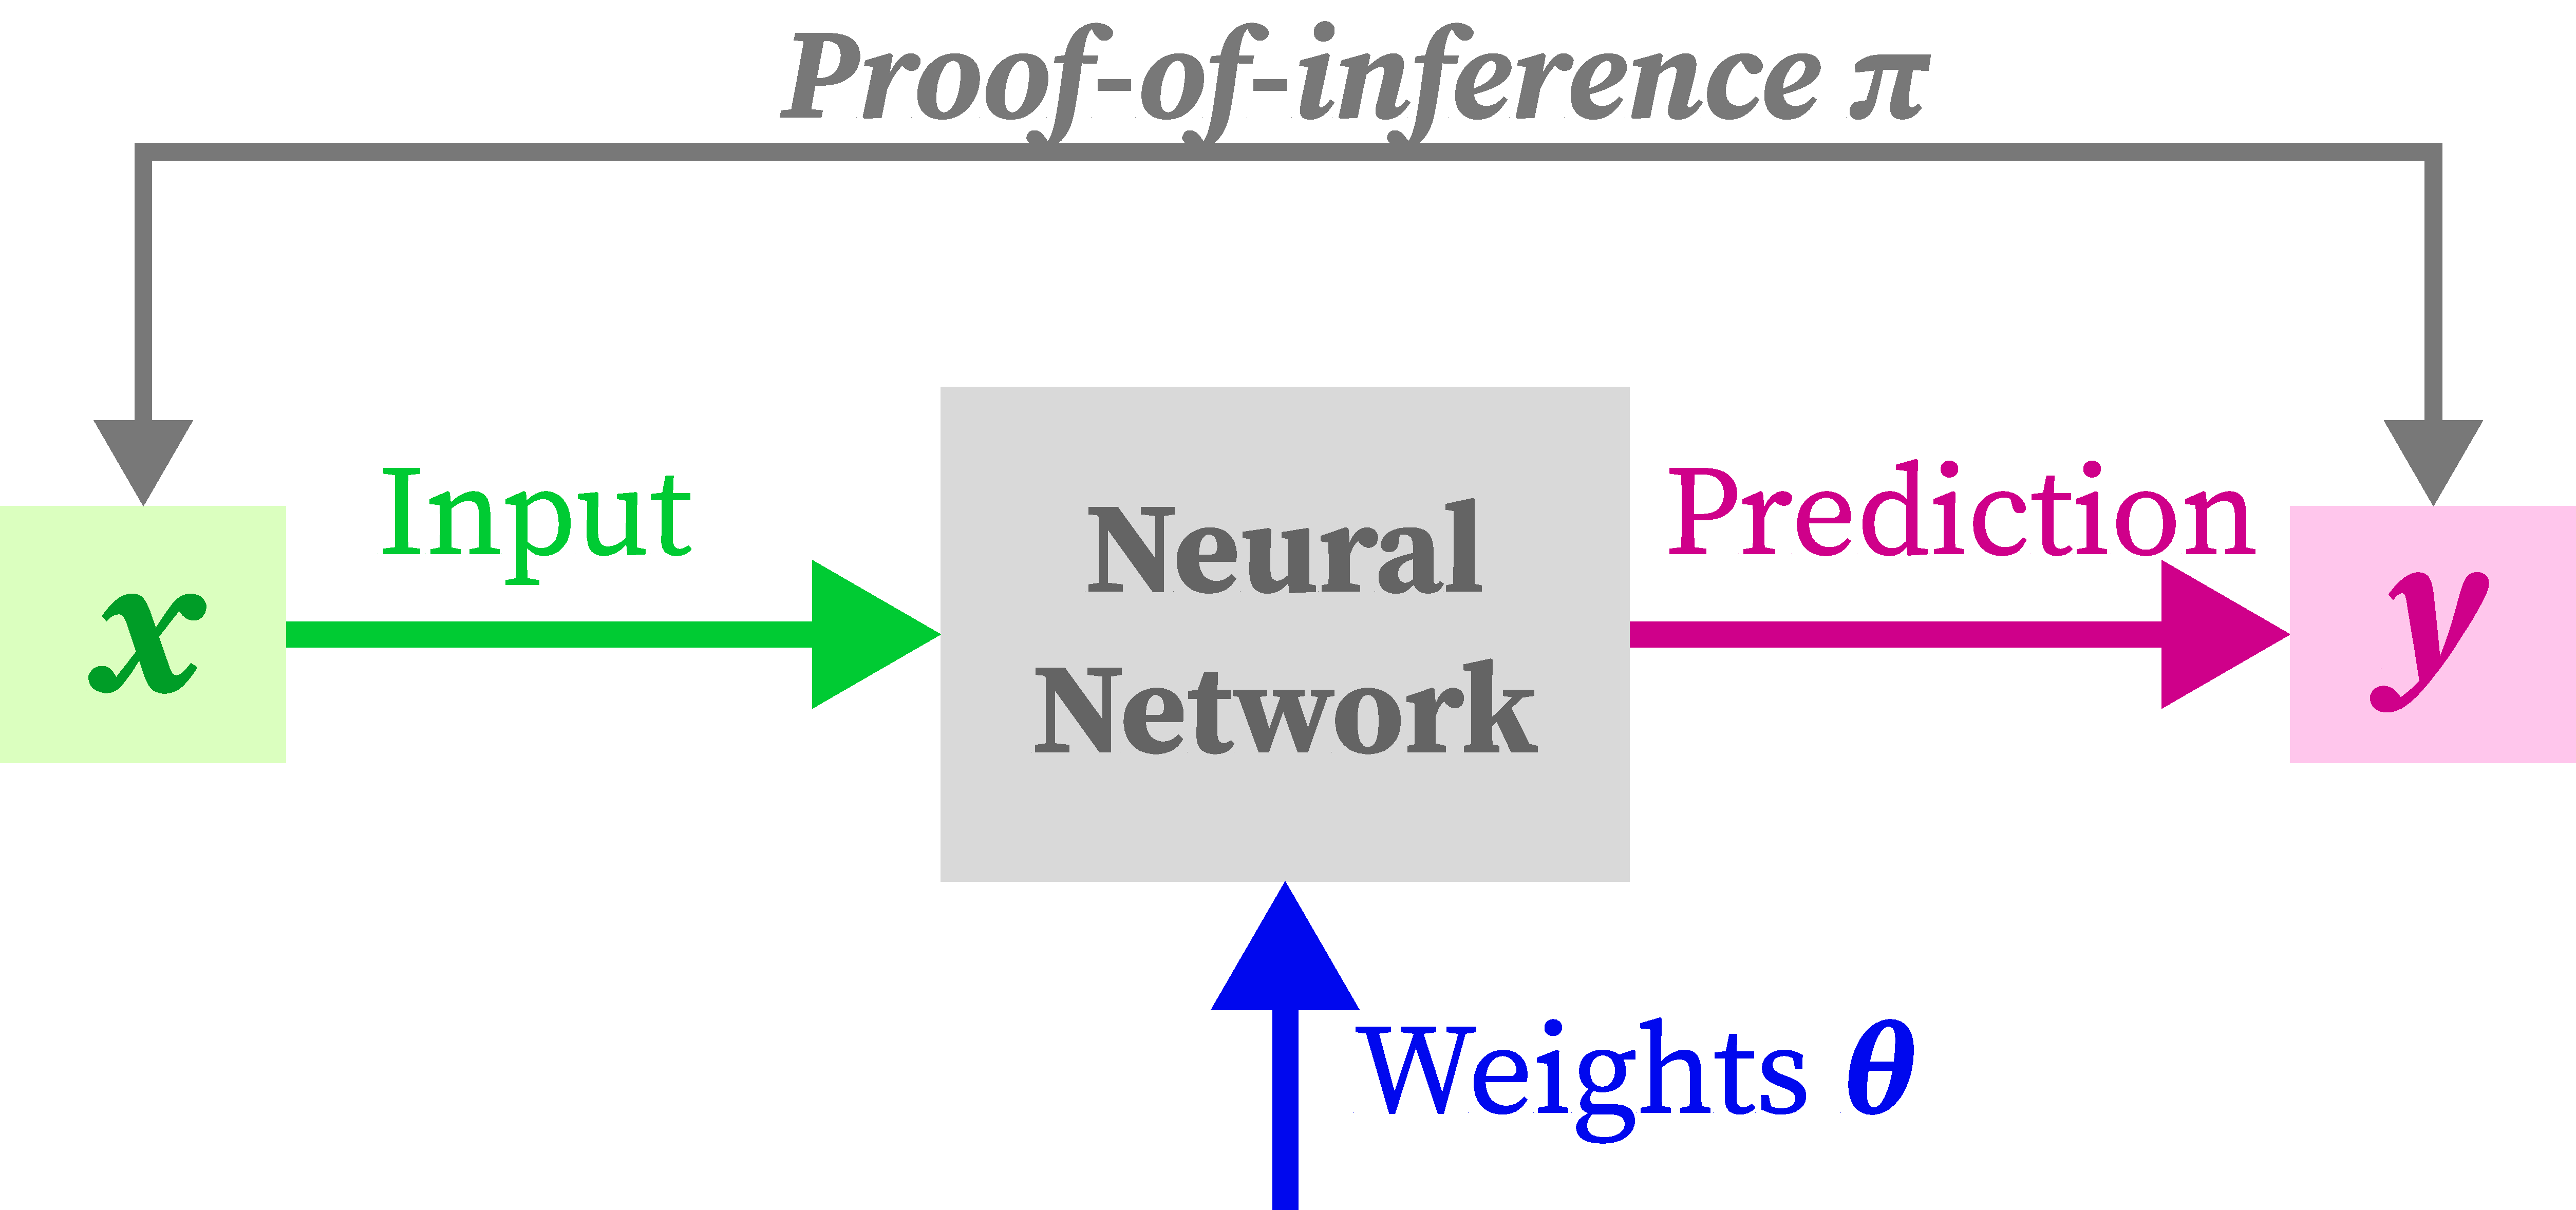
\includegraphics[width=0.85\textwidth]{images/proof-of-inference.pdf}
            \end{figure}
            

            \vspace{15px}
            \begin{center}
                \setlength{\fboxrule}{1.0pt}
                \fcolorbox{blue}{blue!10}{
                    \parbox{0.8\linewidth}{
                        Prove that for $\textcolor{green!50!black}{\boldsymbol{x}},\textcolor{purple}{\boldsymbol{y}},\textcolor{blue}{\boldsymbol{\theta}}$ we indeed have $\textcolor{purple}{\boldsymbol{y}} = \textcolor{gray!80!black}{f}(\textcolor{green!60!black}{\boldsymbol{x}};\textcolor{blue}{\boldsymbol{\theta}})$.
                    }
                }
            \end{center}
        }

        \only<3>{
            Yet, what is public and what is private? Obviously, $\textcolor{purple}{\boldsymbol{y}}$ is public, so what about $\textcolor{green!50!black}{\boldsymbol{x}}$ and $\textcolor{blue}{\boldsymbol{\theta}}$?
        }
    \end{frame}

    \begin{frame}{ZKML: Private \textcolor{blue}{Weights $\theta$}, Public \textcolor{green!50!black}{Input $x$}}
        \only<1>{
            \begin{figure}
                \centering
                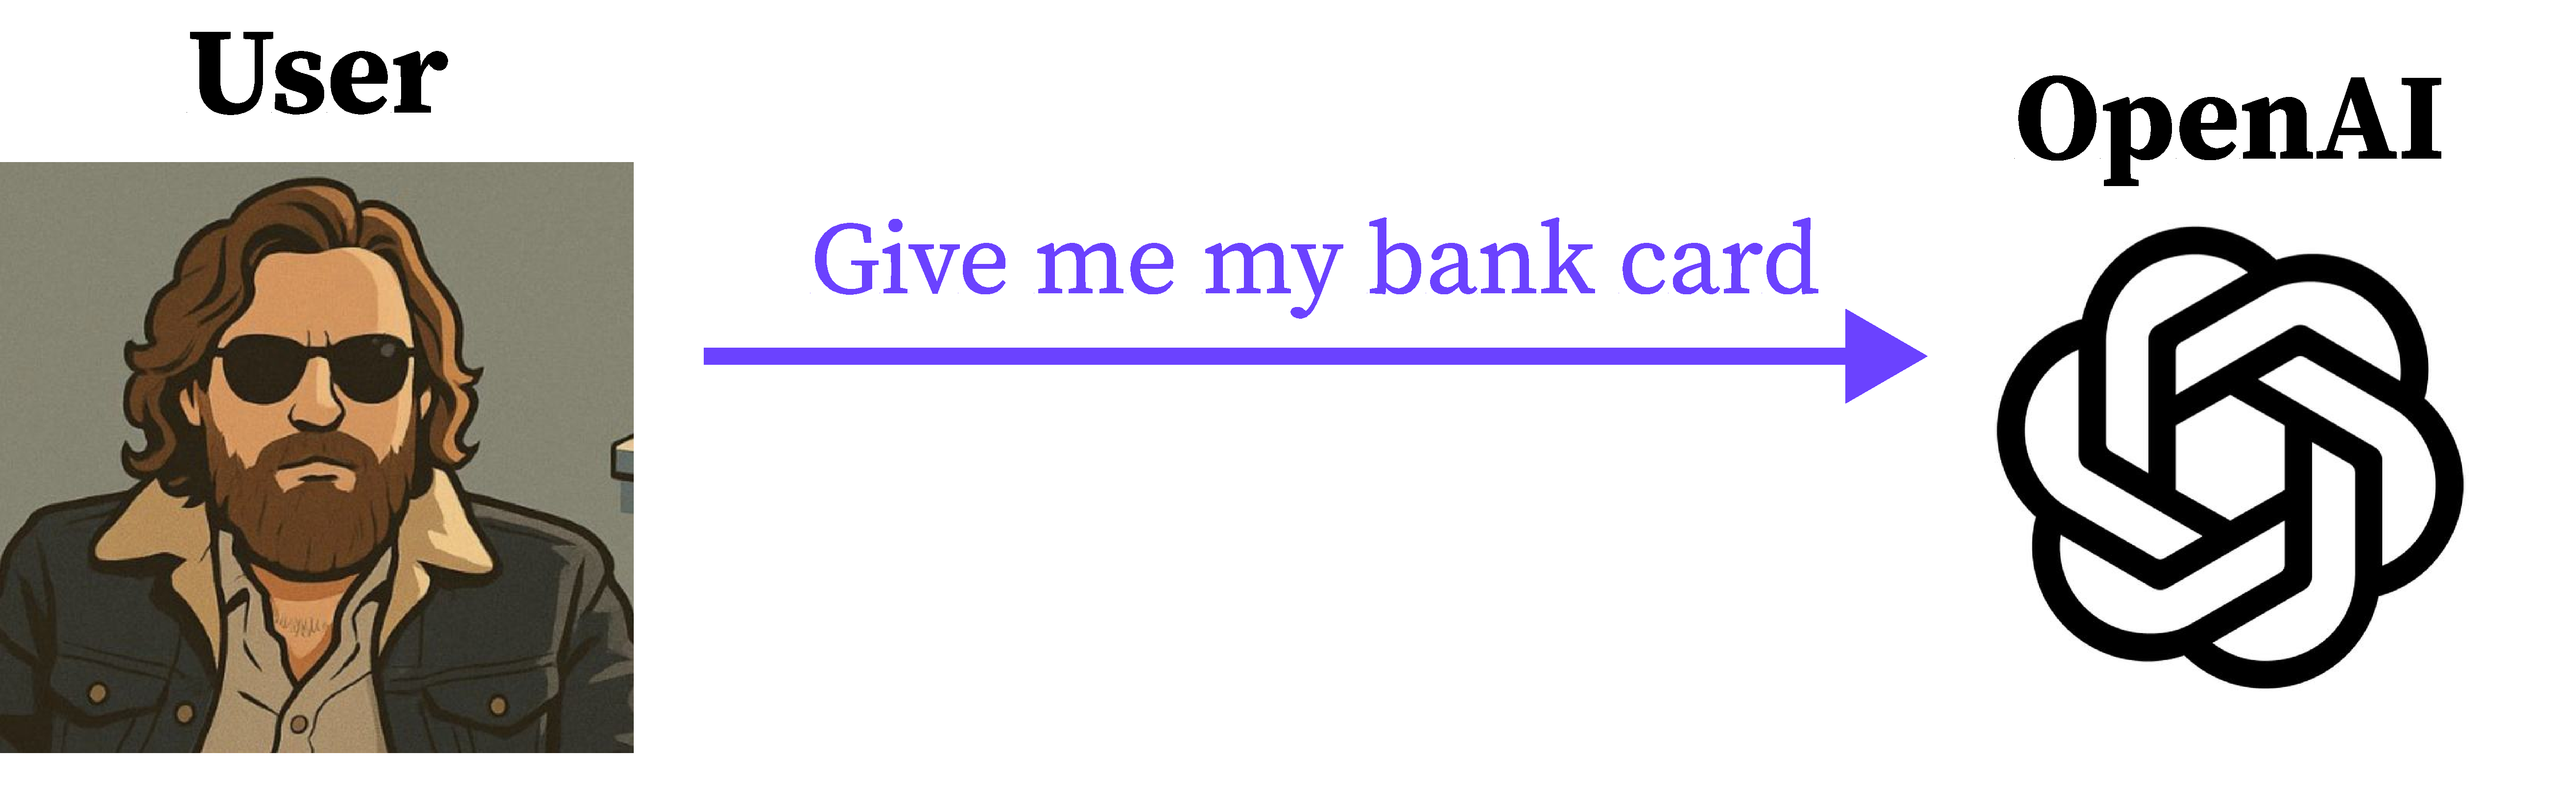
\includegraphics[width=0.85\textwidth]{images/private_weights_1.pdf}
            \end{figure}
        }
        \only<2>{
            \begin{figure}
                \centering
                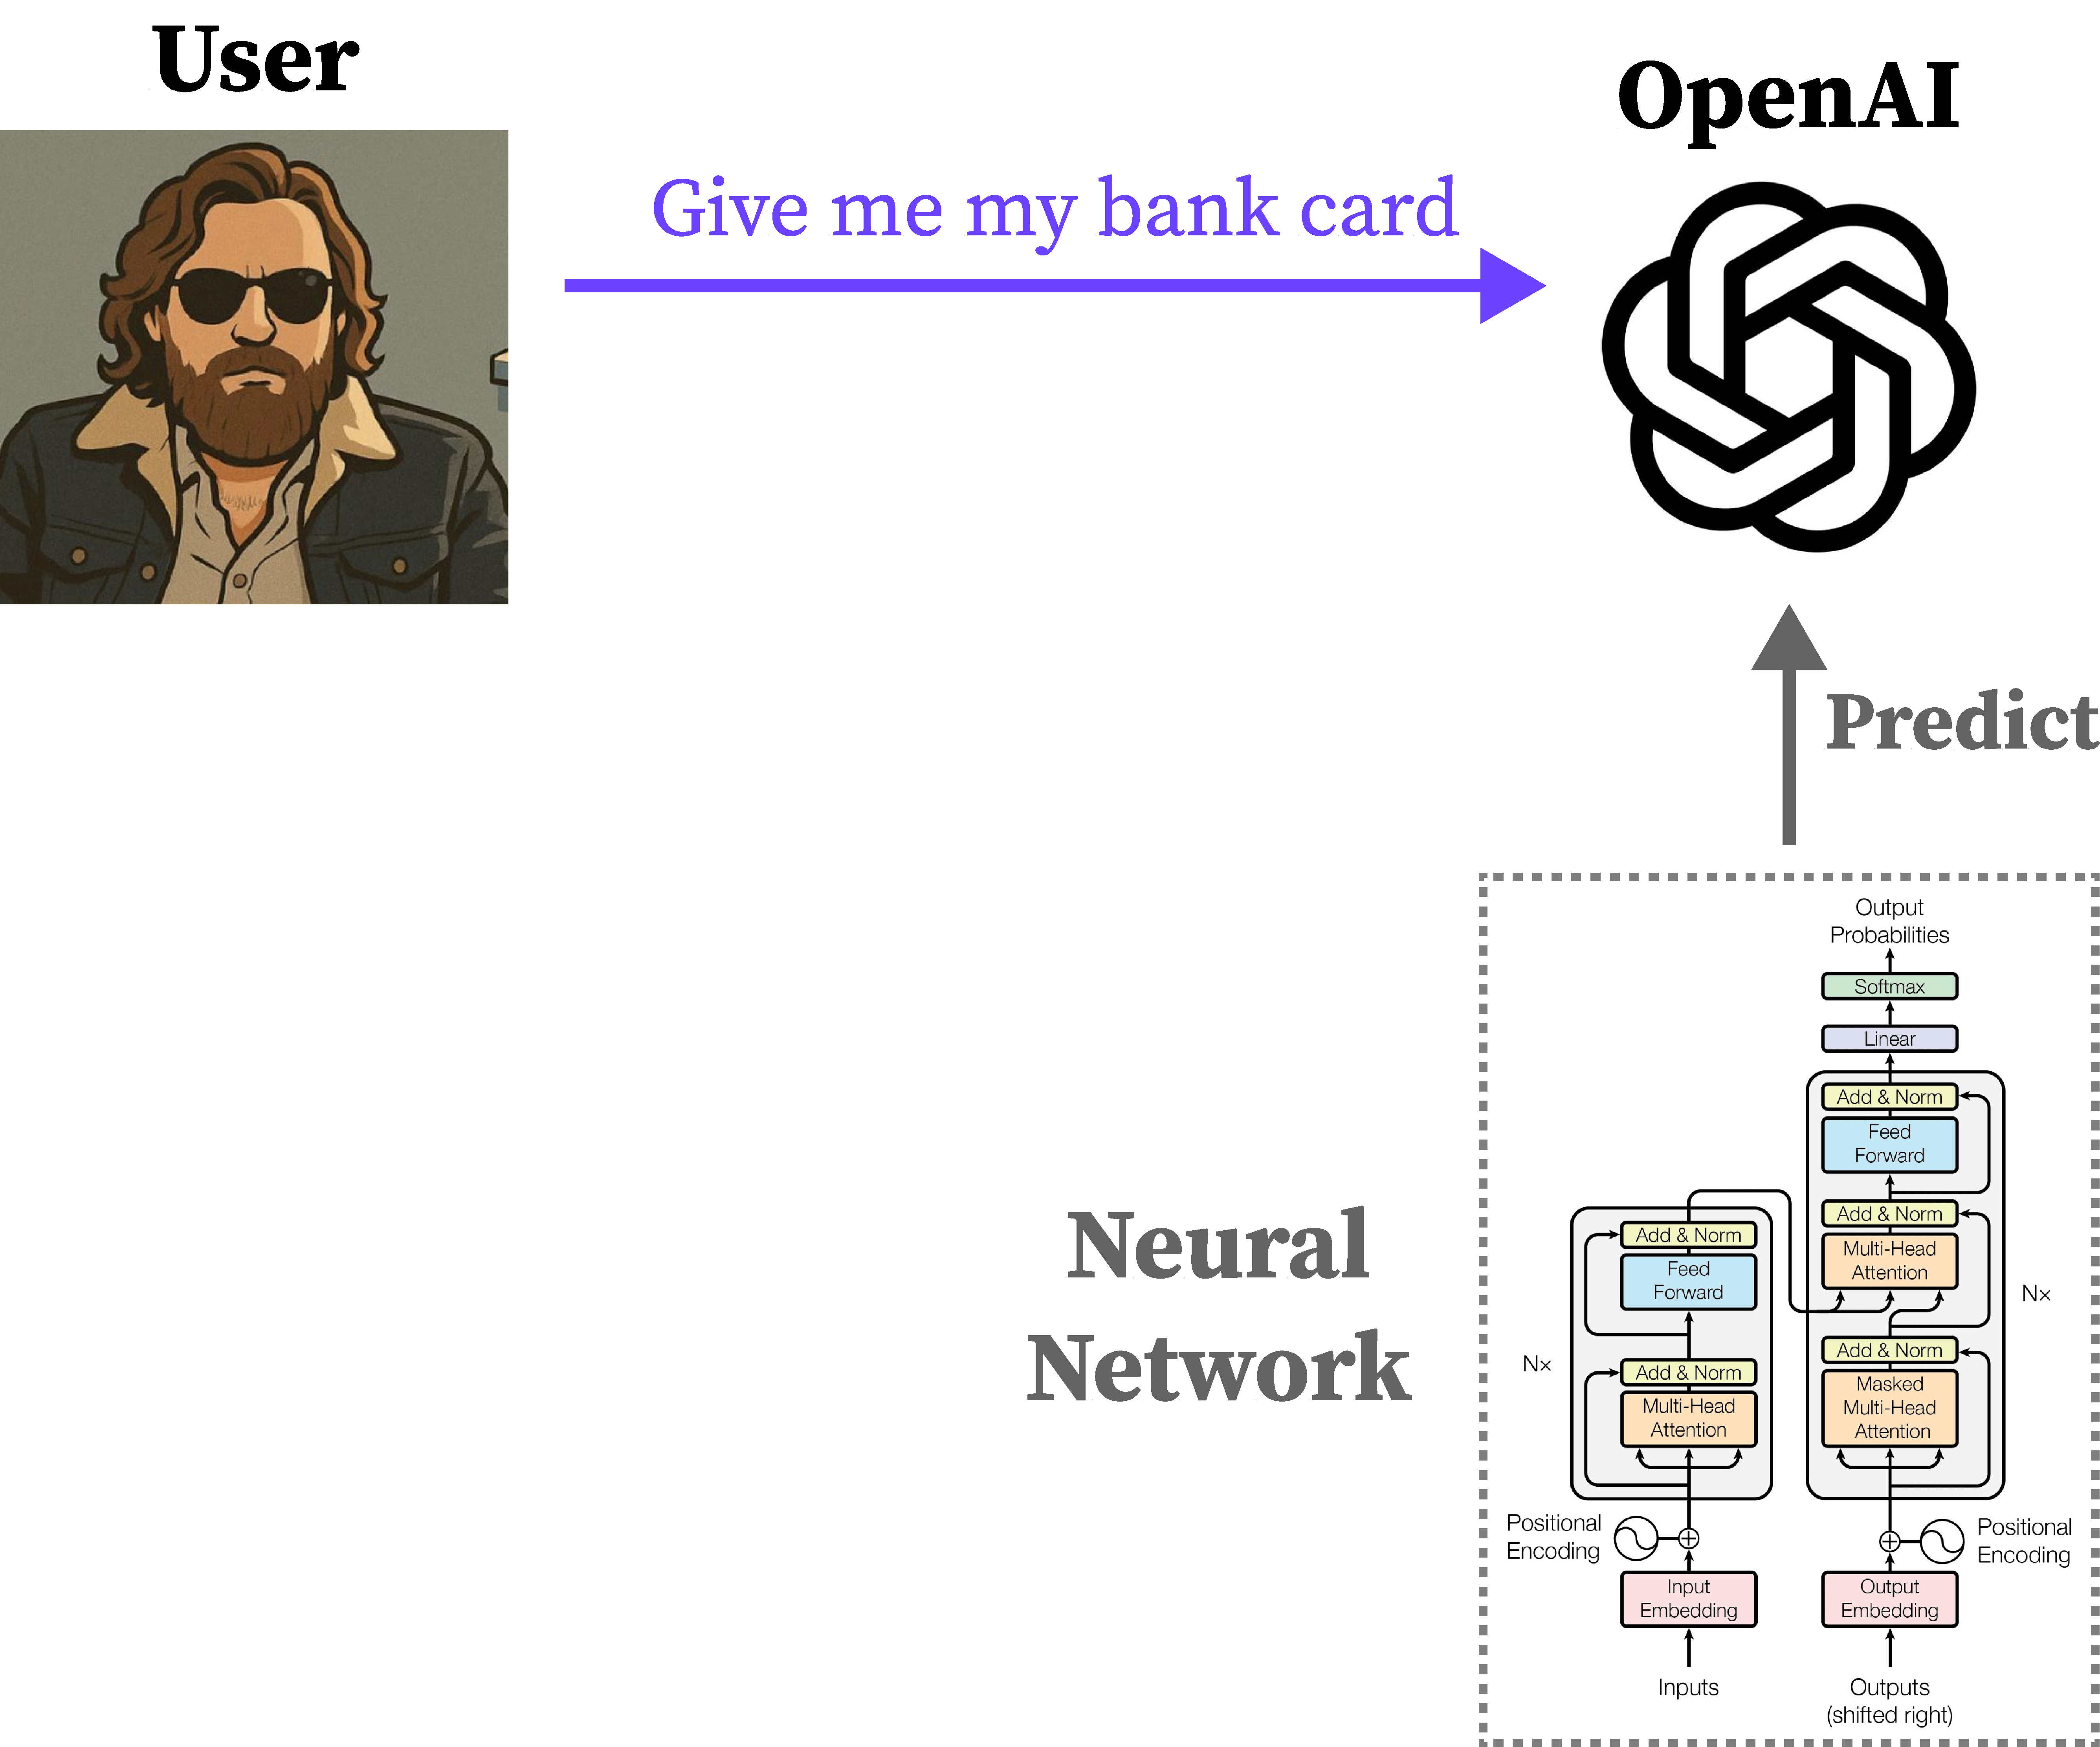
\includegraphics[width=0.85\textwidth]{images/private_weights_2.pdf}
            \end{figure}
        }
        \only<3>{
            \begin{figure}
                \centering
                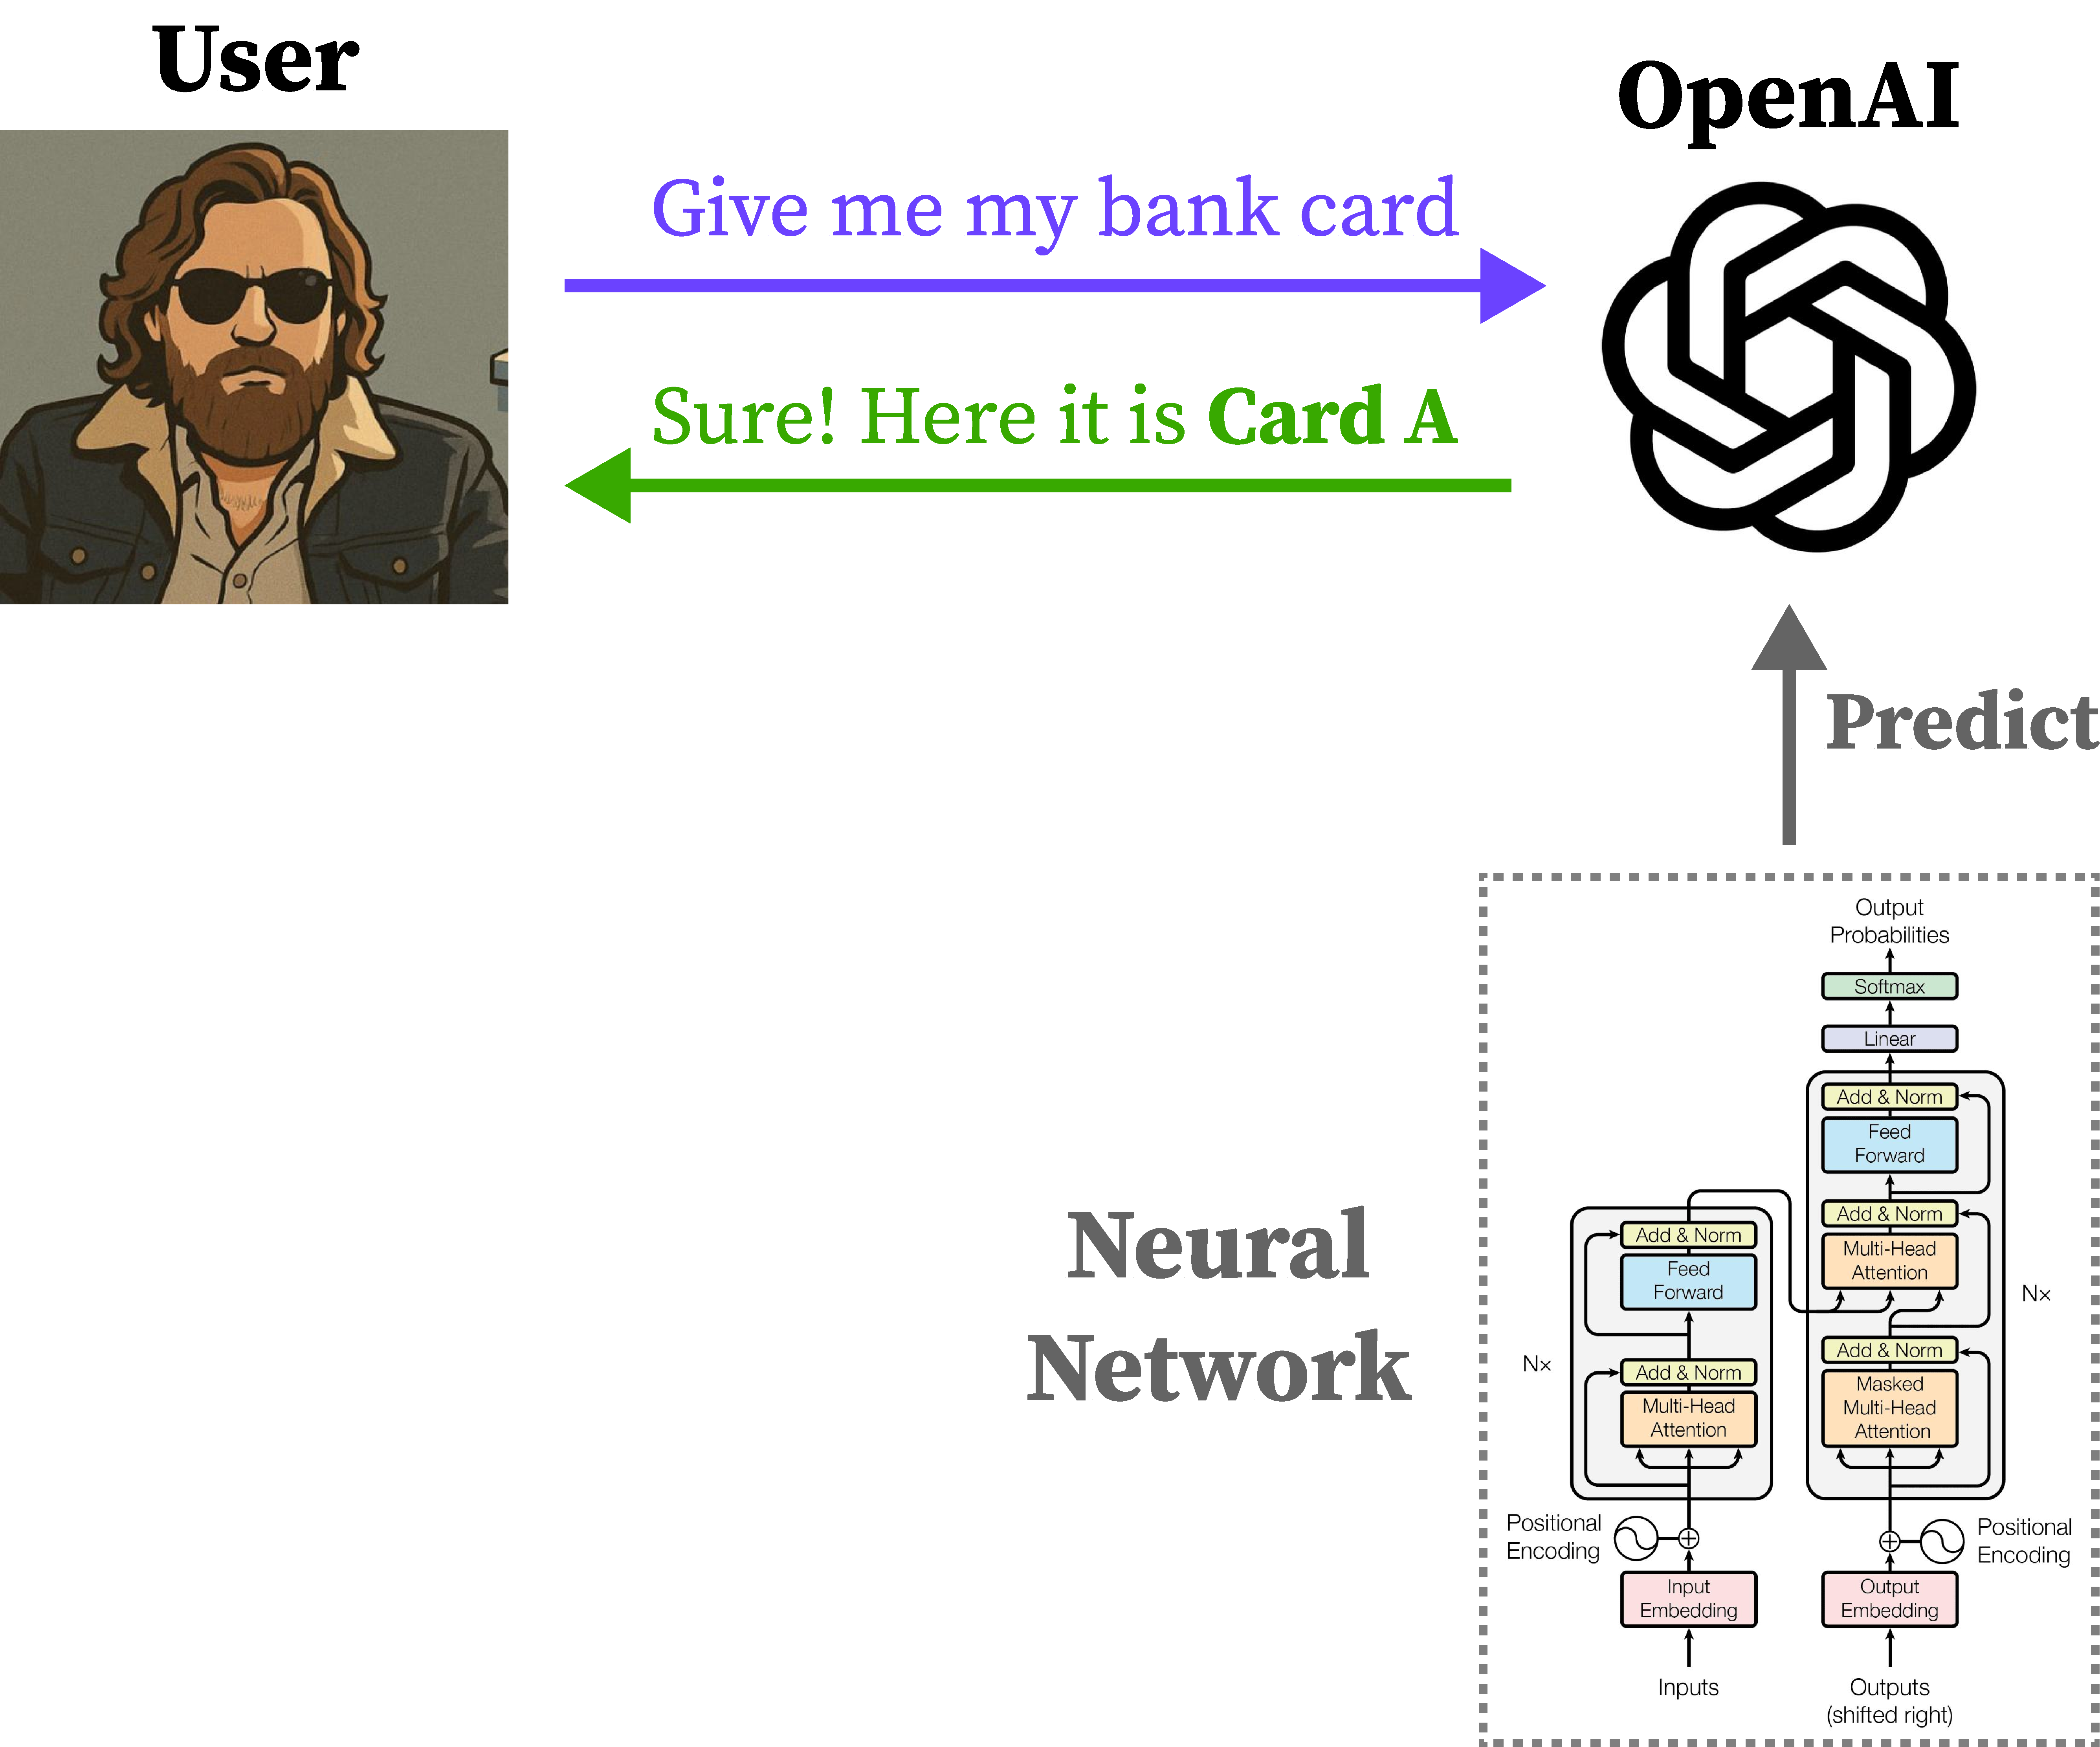
\includegraphics[width=0.85\textwidth]{images/private_weights_3.pdf}
            \end{figure}
        }
        \only<4>{
            \begin{figure}
                \centering
                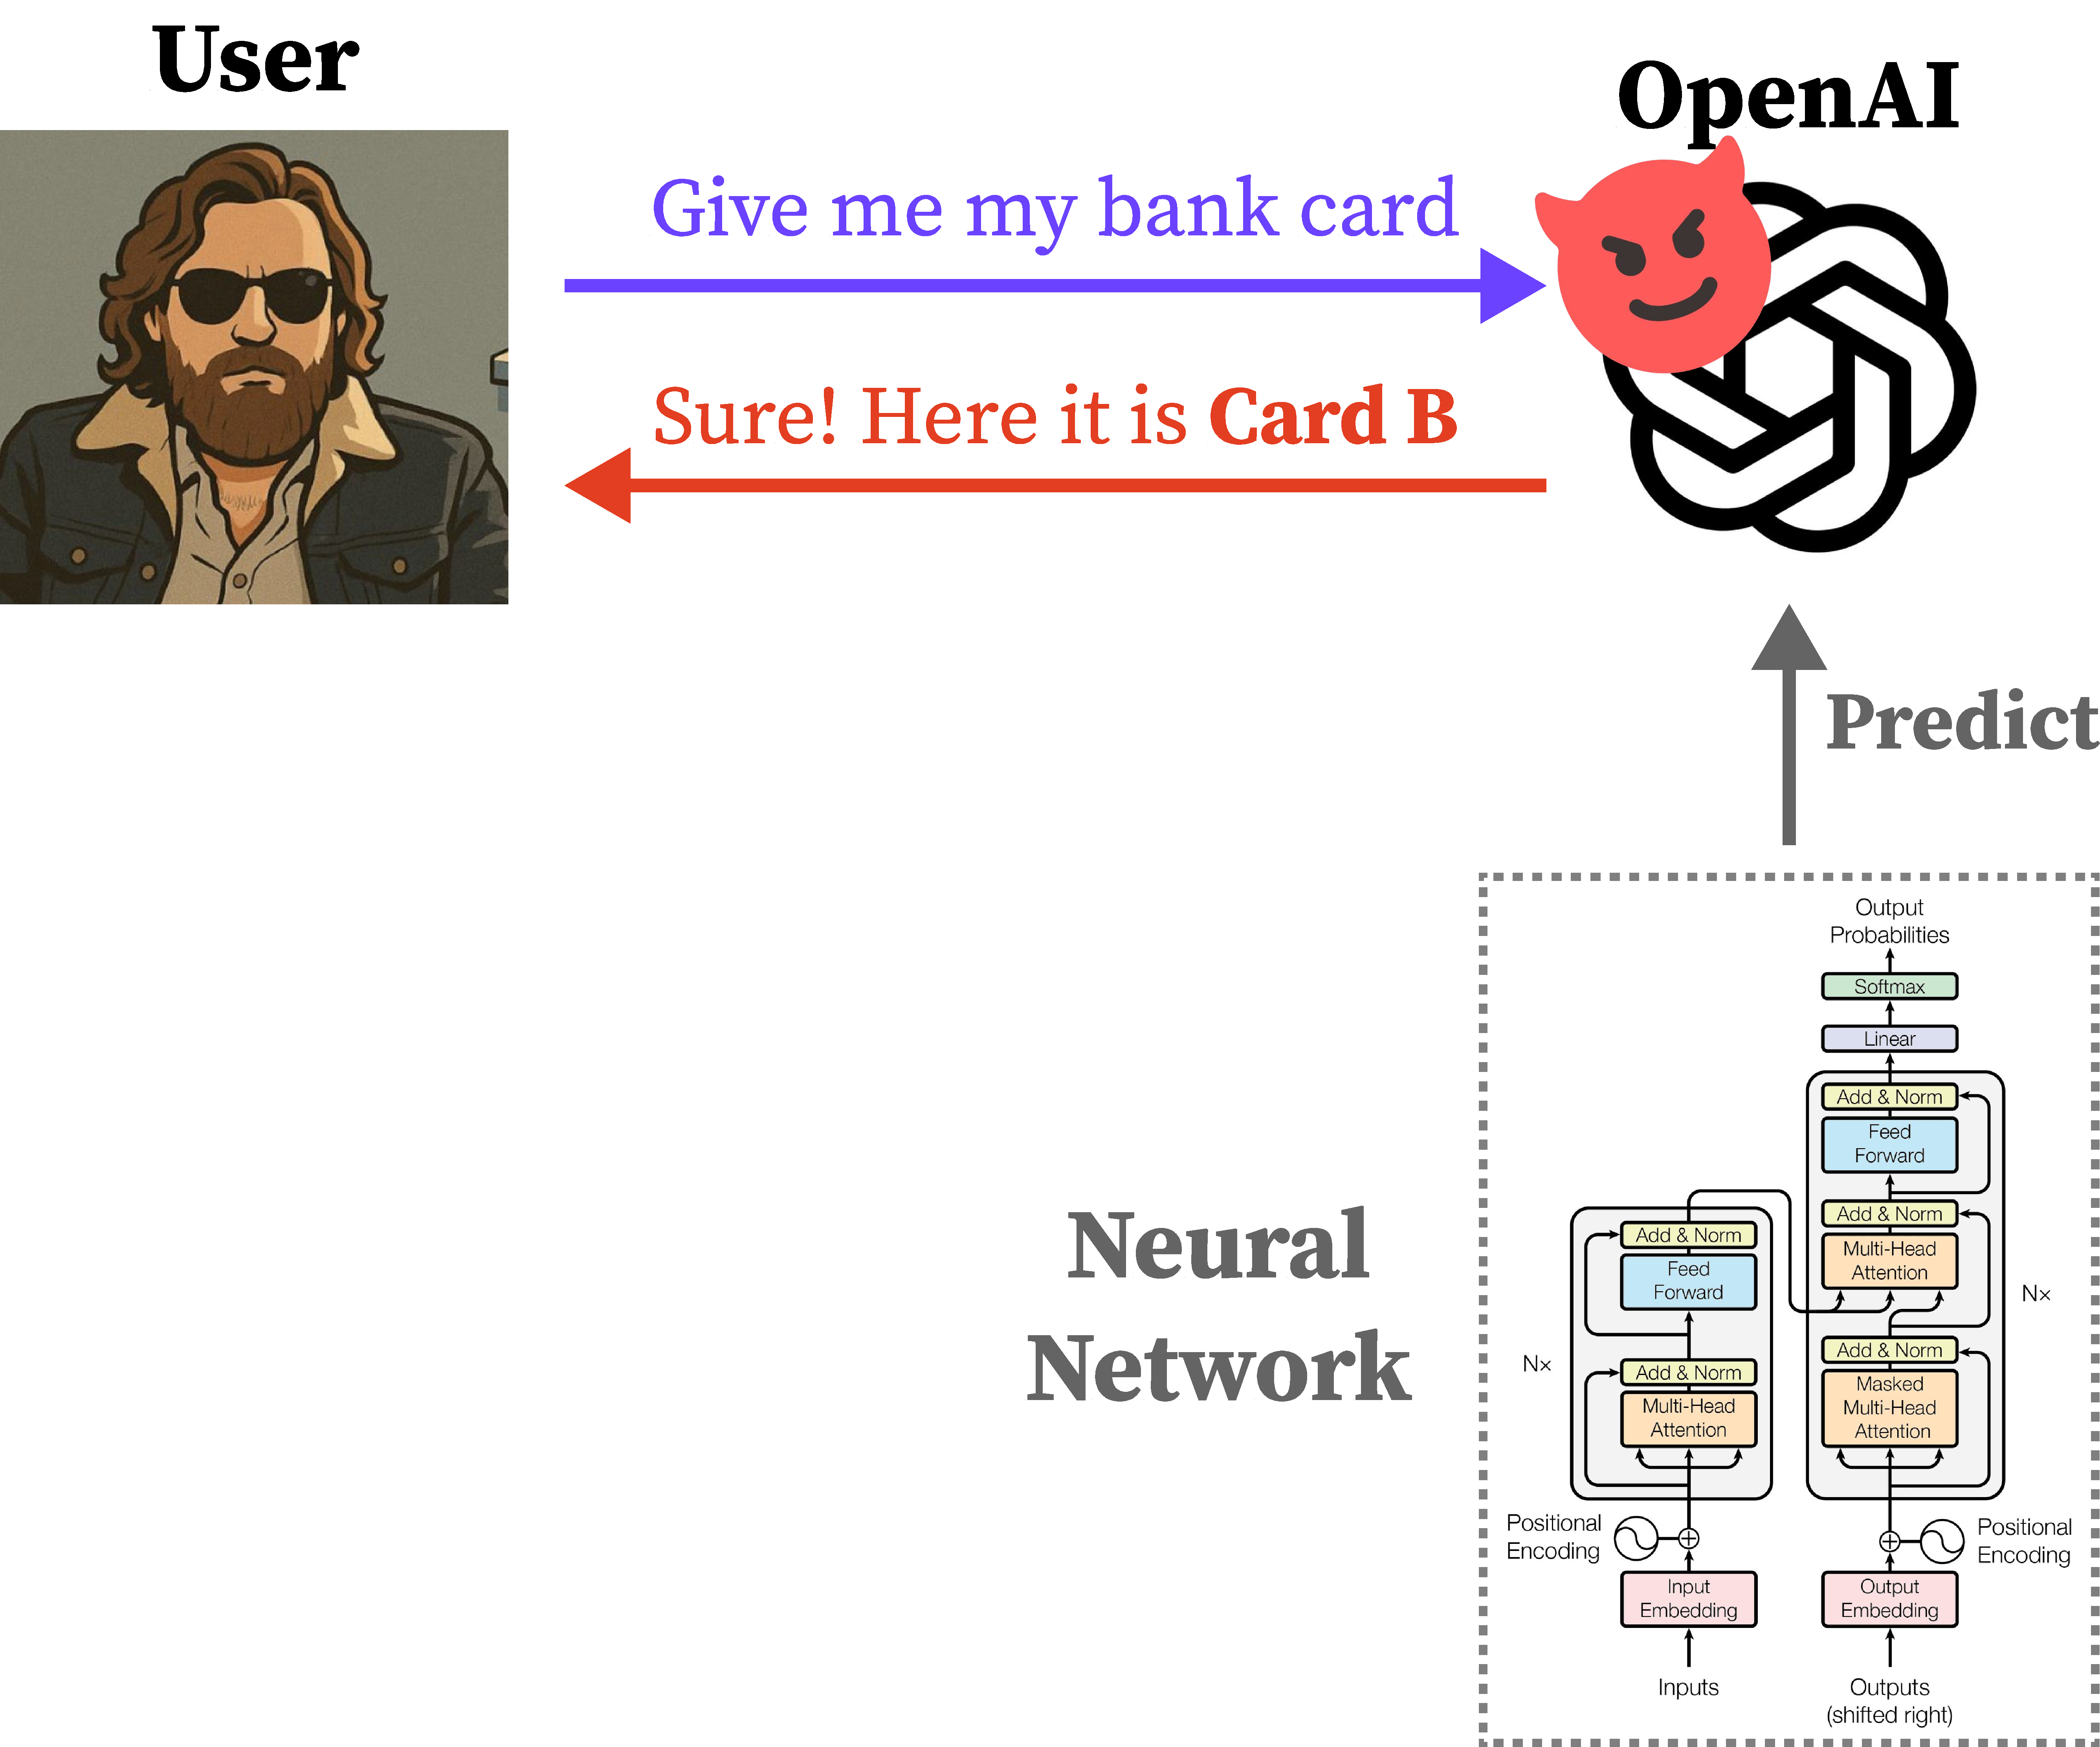
\includegraphics[width=0.85\textwidth]{images/private_weights_4.pdf}
            \end{figure}
        }
        \only<5>{
            \begin{figure}
                \centering
                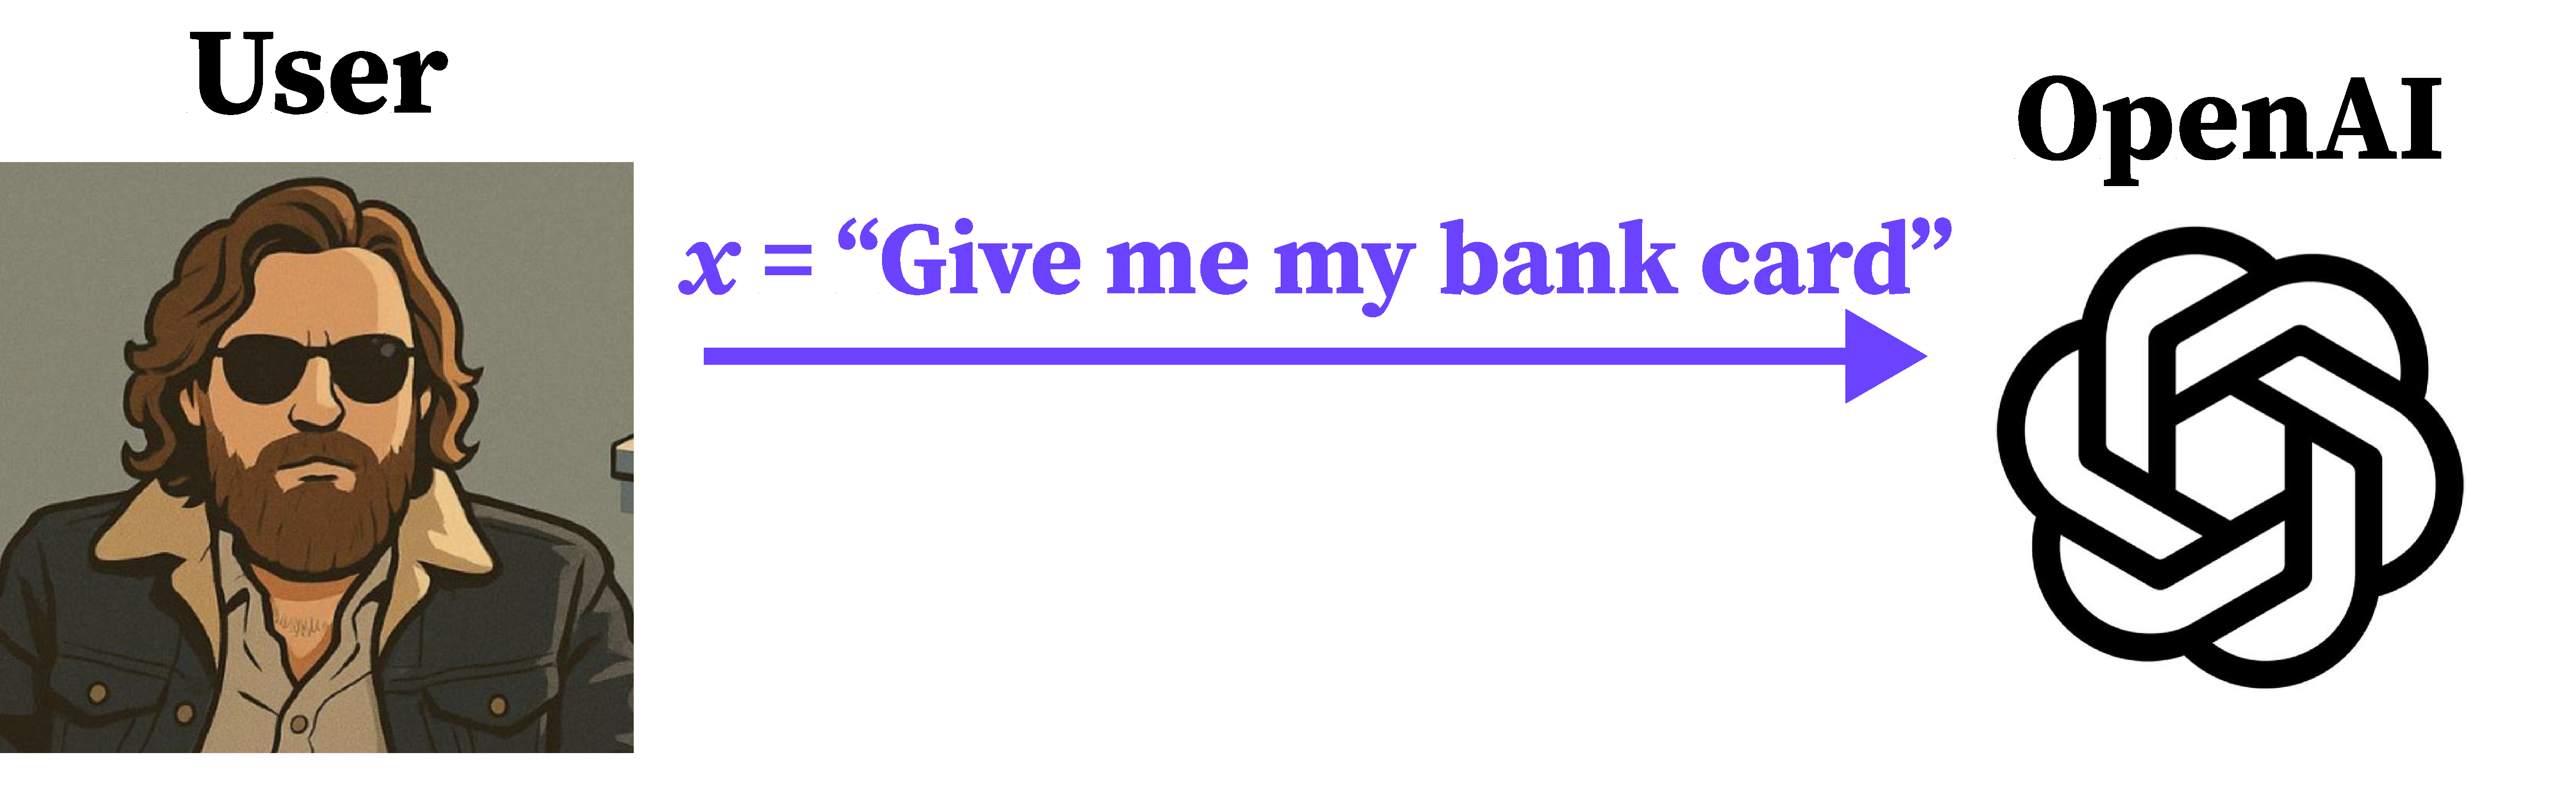
\includegraphics[width=0.85\textwidth]{images/private_weights_5.pdf}
            \end{figure}
        }
        \only<6>{
            \begin{figure}
                \centering
                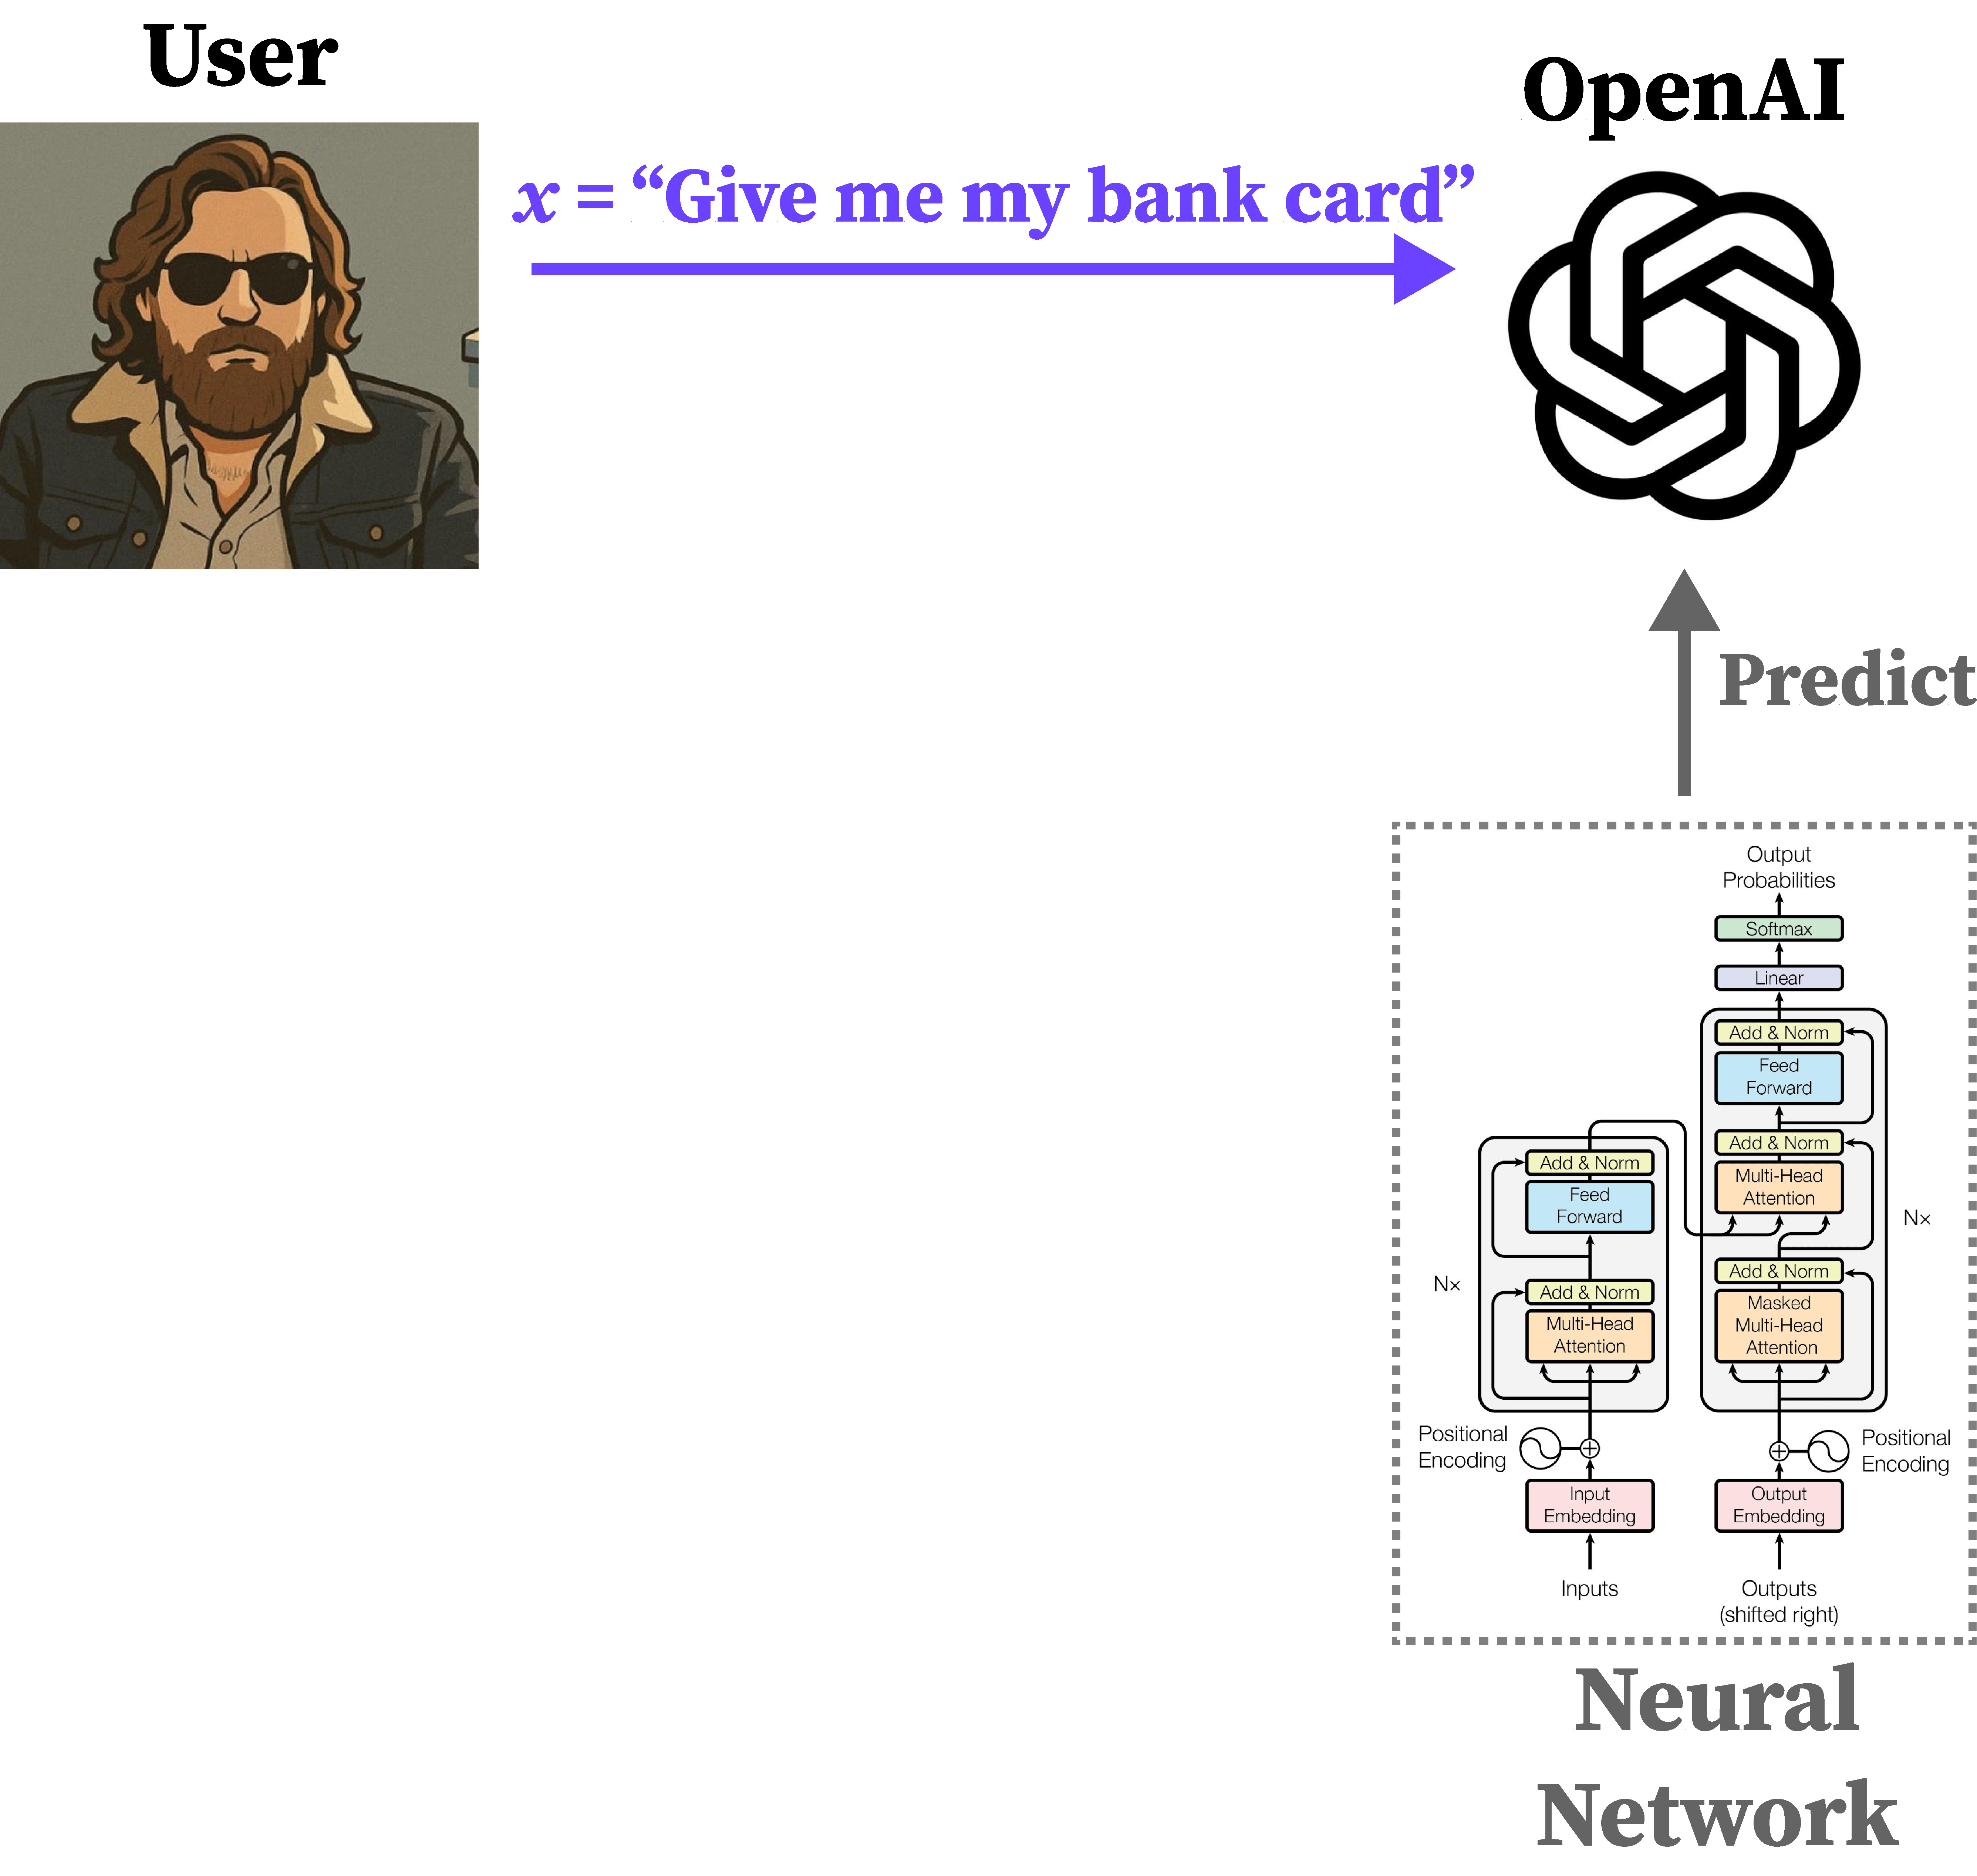
\includegraphics[width=0.75\textwidth]{images/private_weights_6.pdf}
            \end{figure}
        }
        \only<7>{
            \begin{figure}
                \centering
                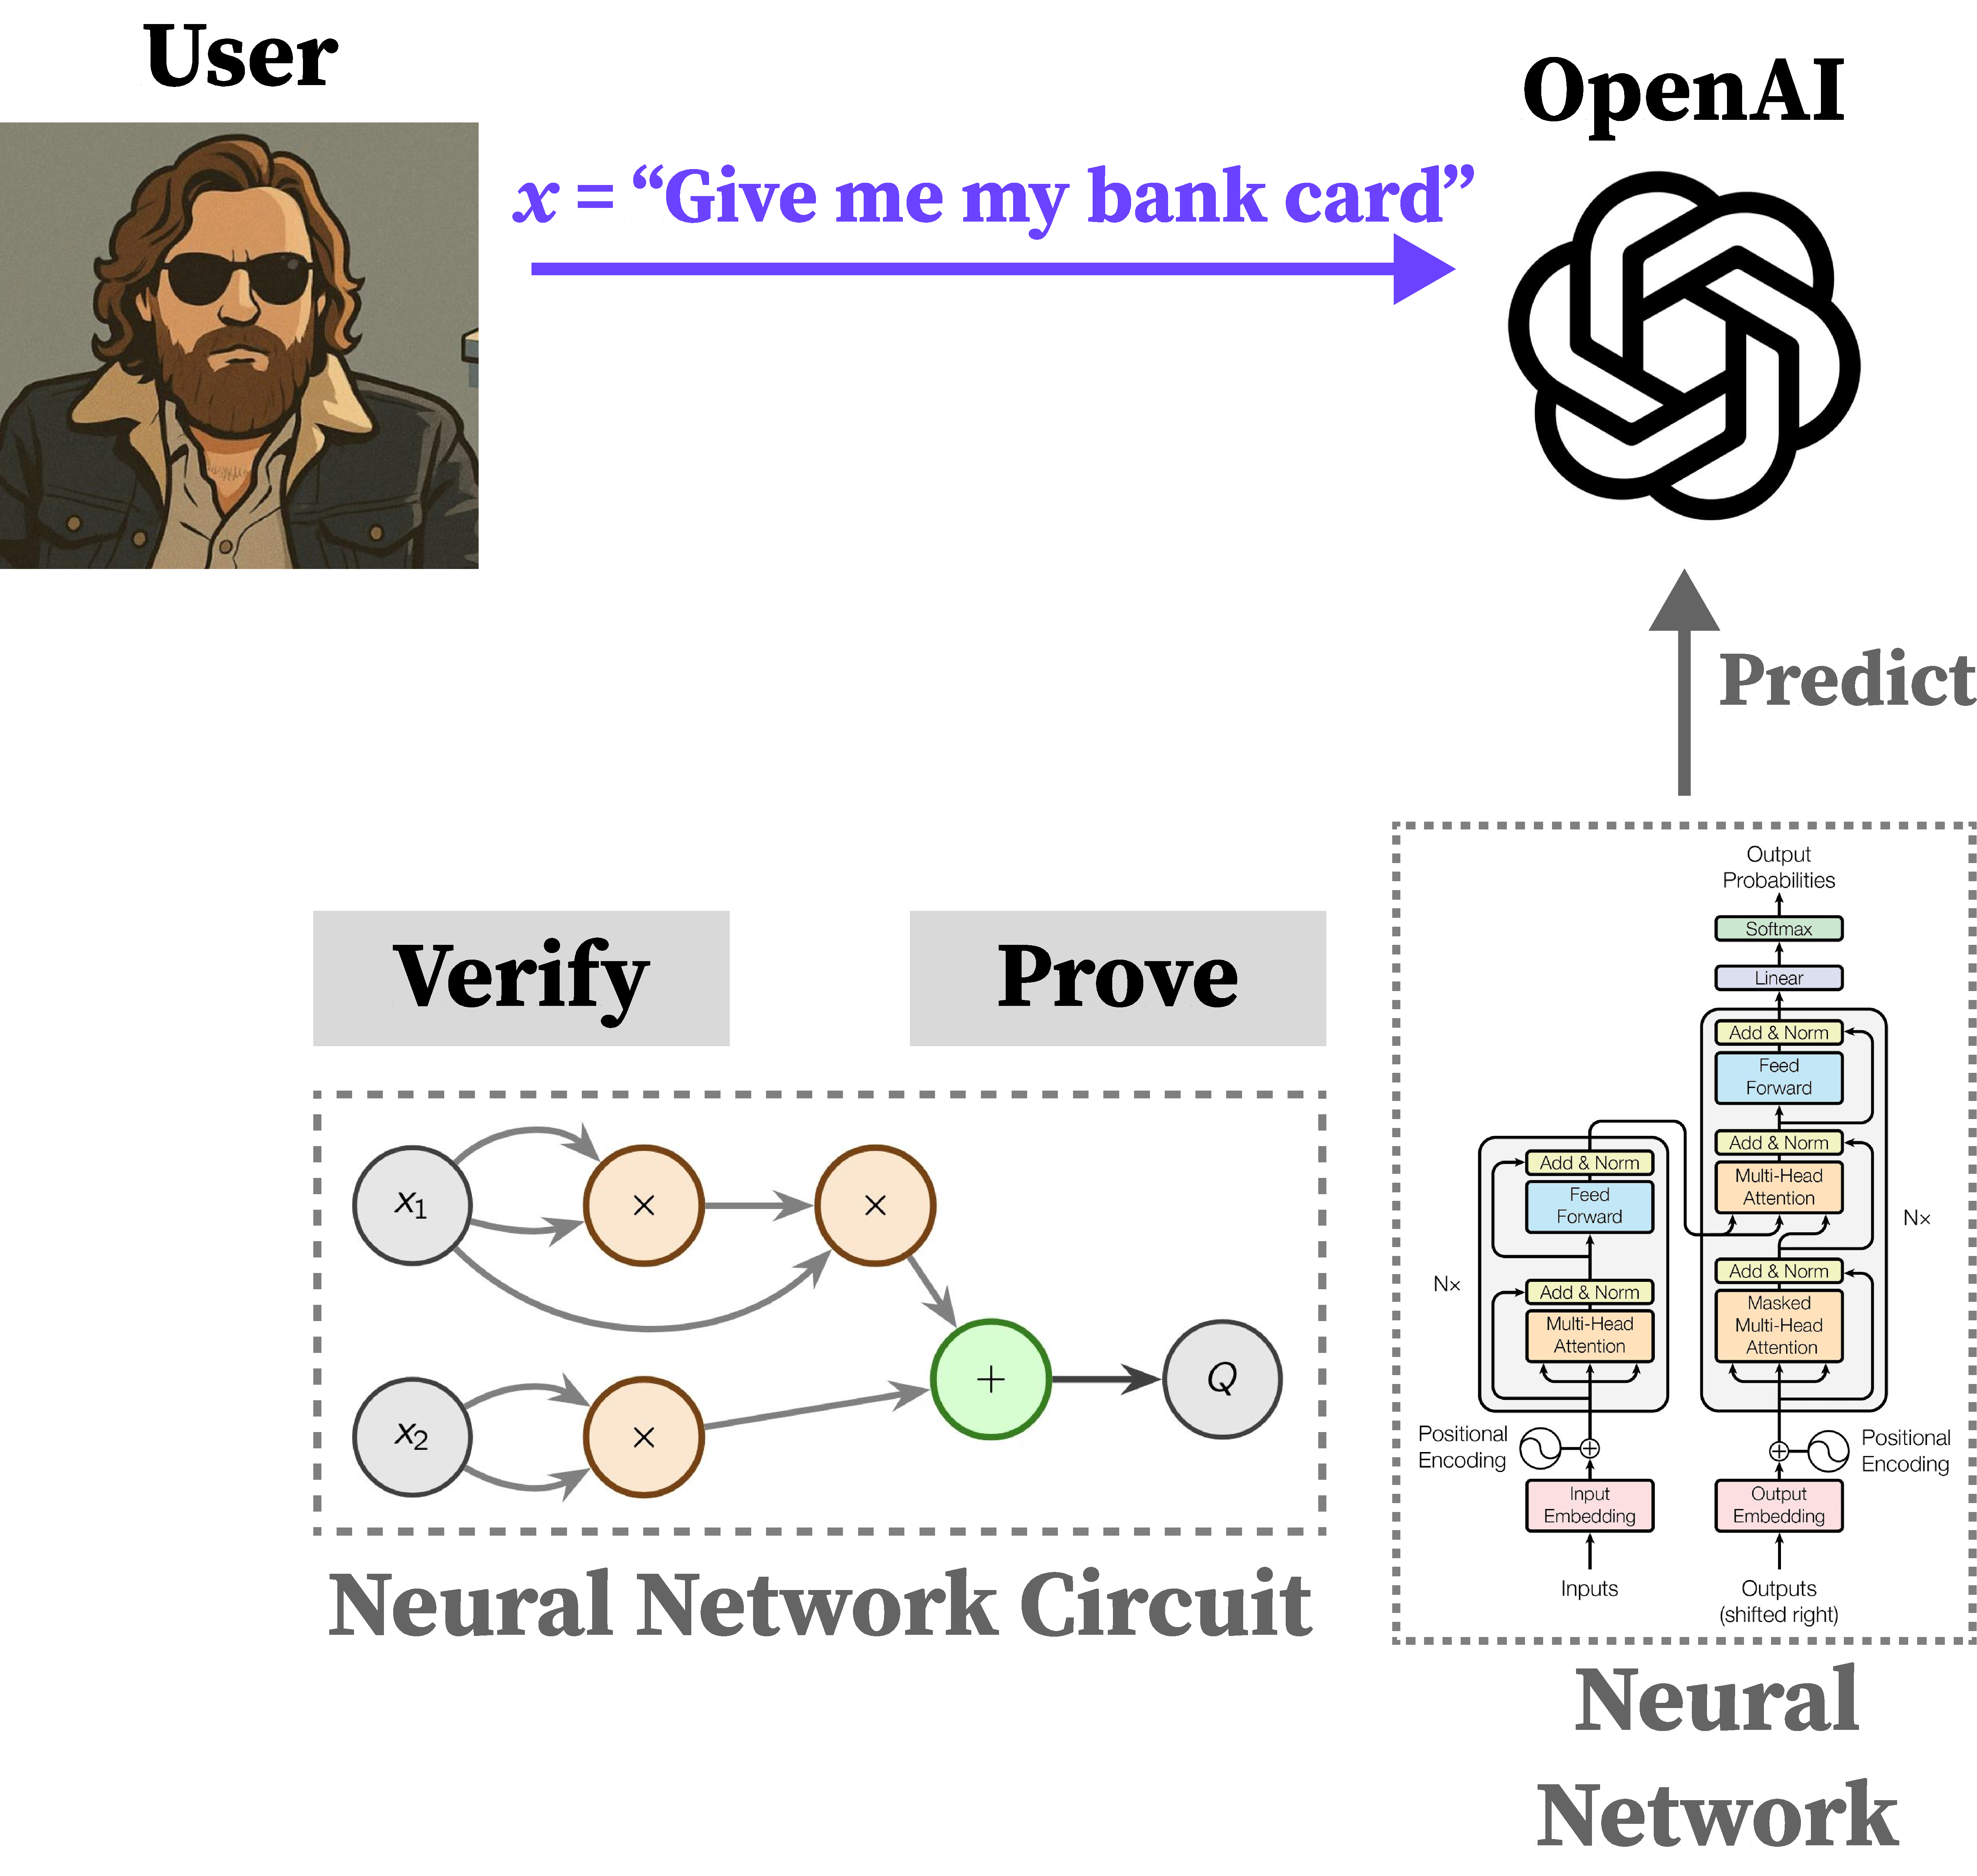
\includegraphics[width=0.75\textwidth]{images/private_weights_7.pdf}
            \end{figure}
        }
        \only<8>{
            \begin{figure}
                \centering
                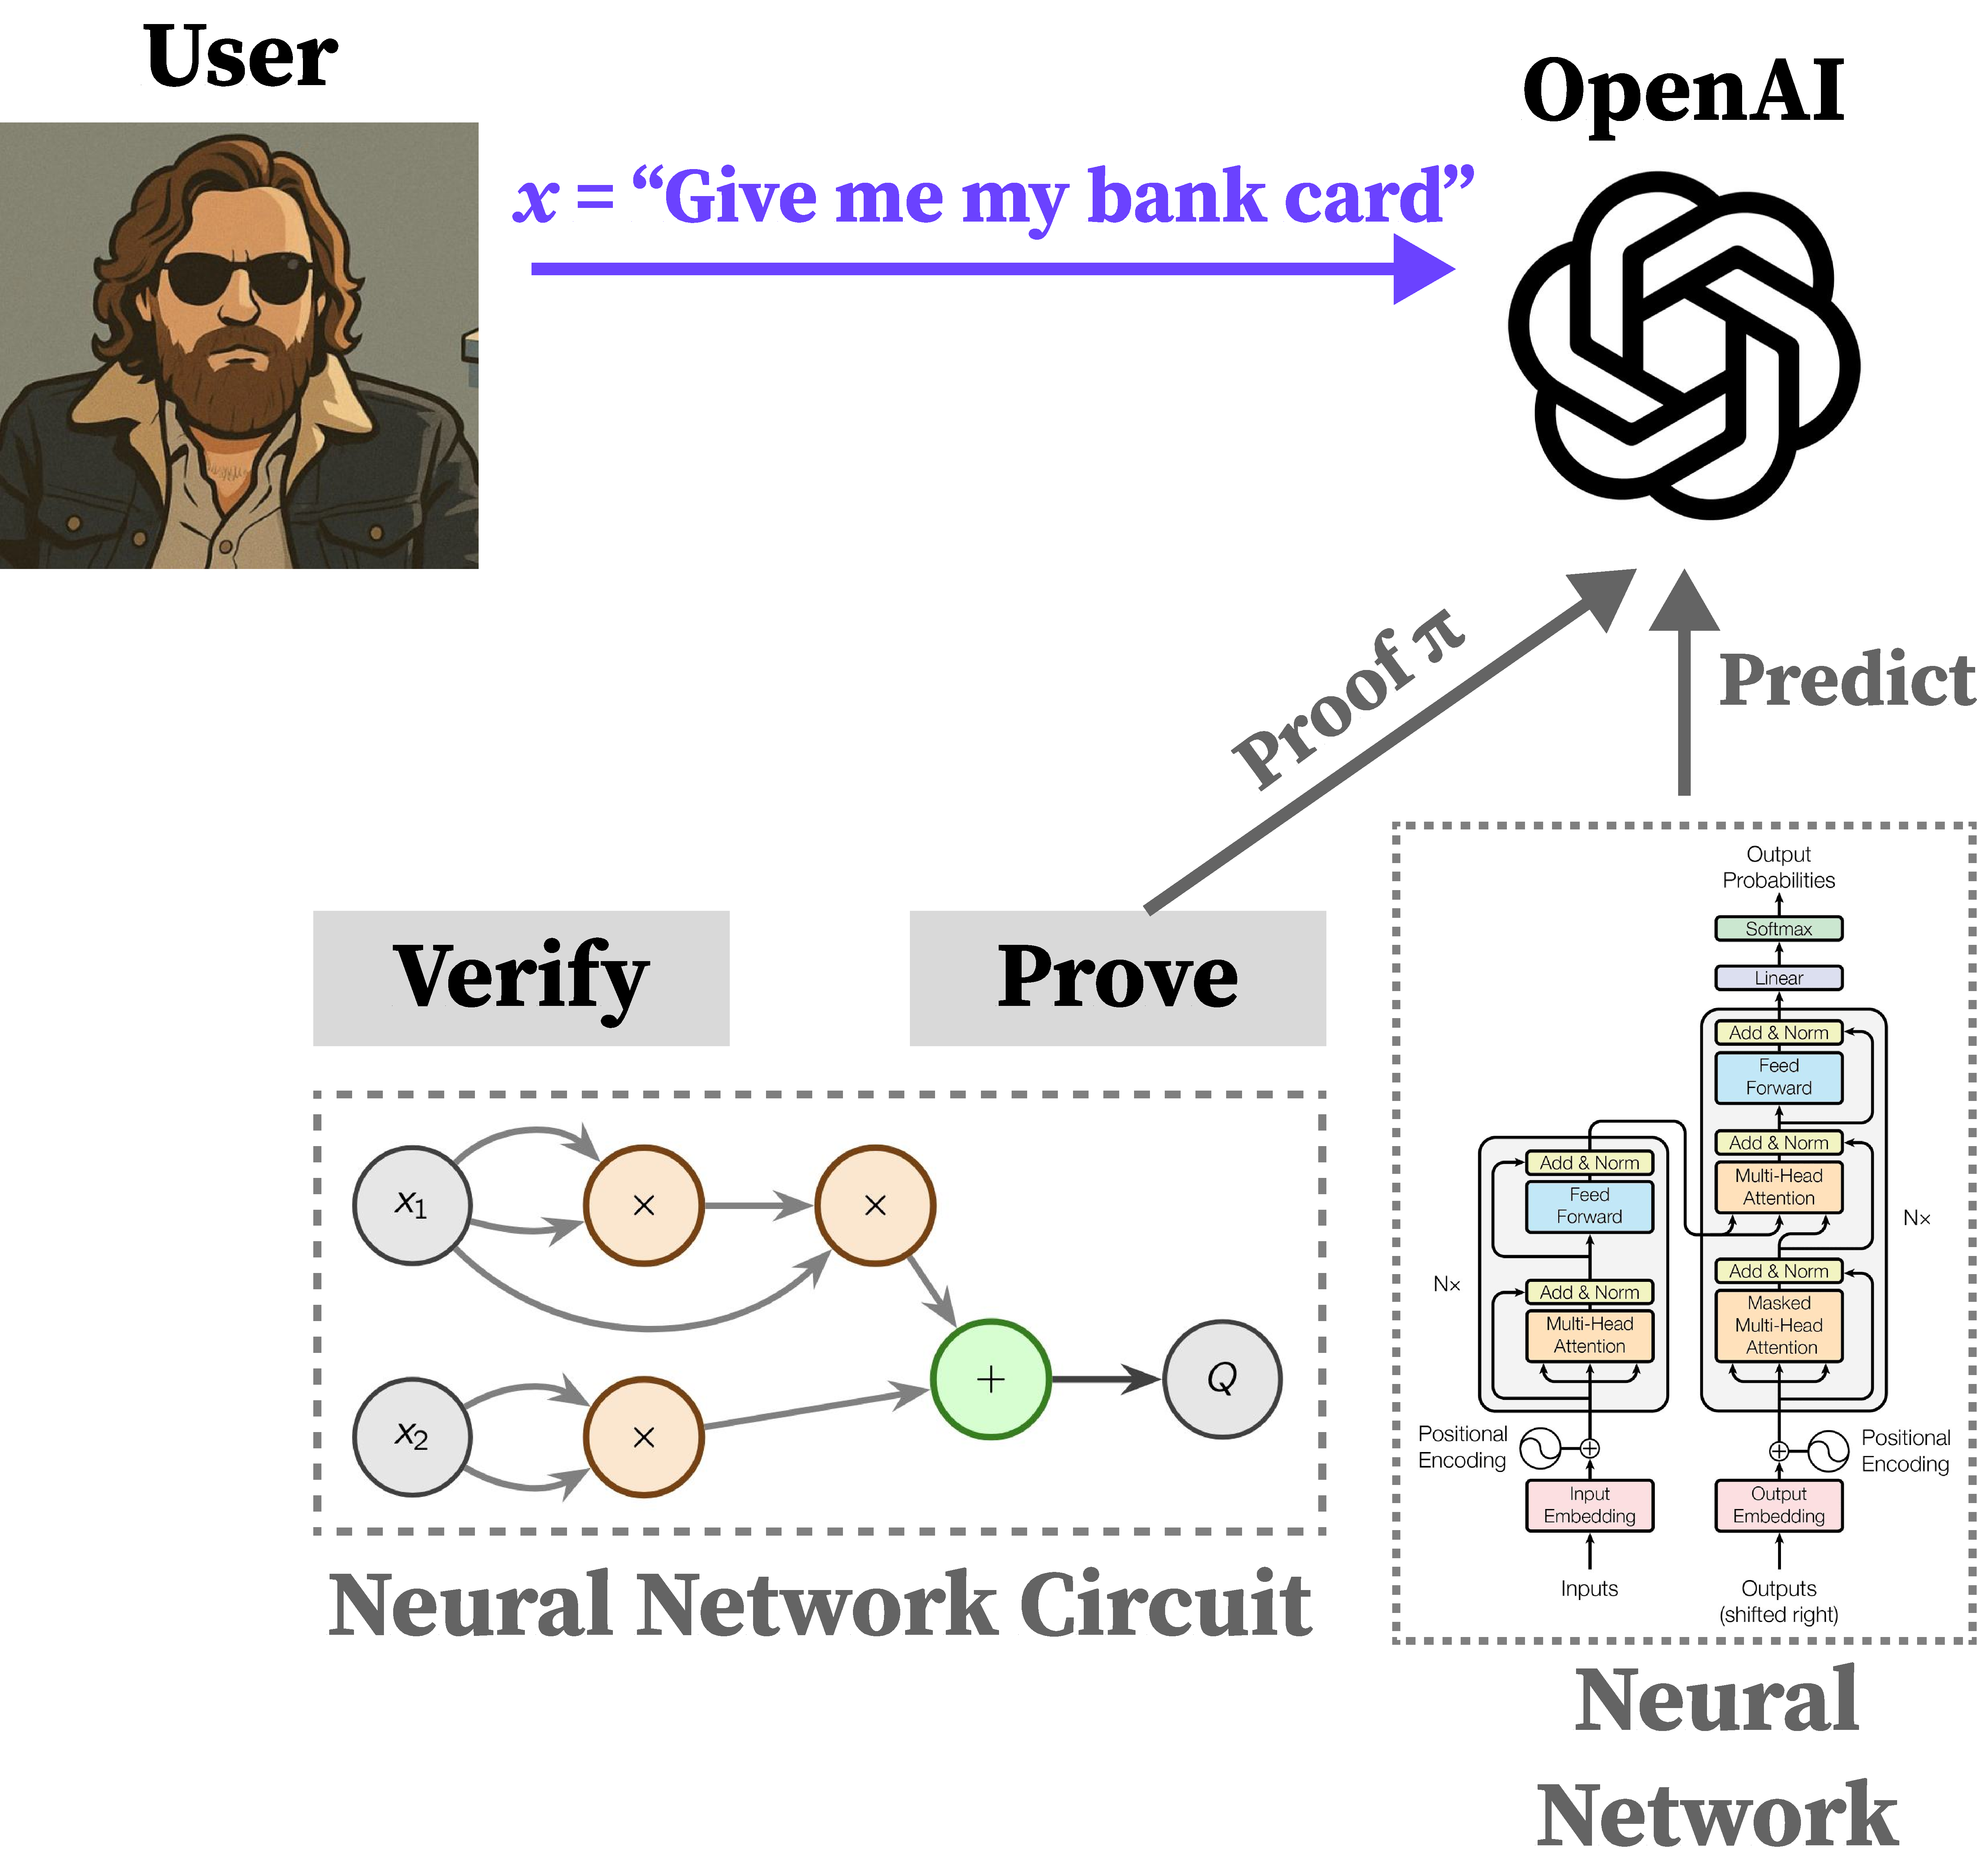
\includegraphics[width=0.75\textwidth]{images/private_weights_8.pdf}
            \end{figure}
        }
        \only<9>{
            \begin{figure}
                \centering
                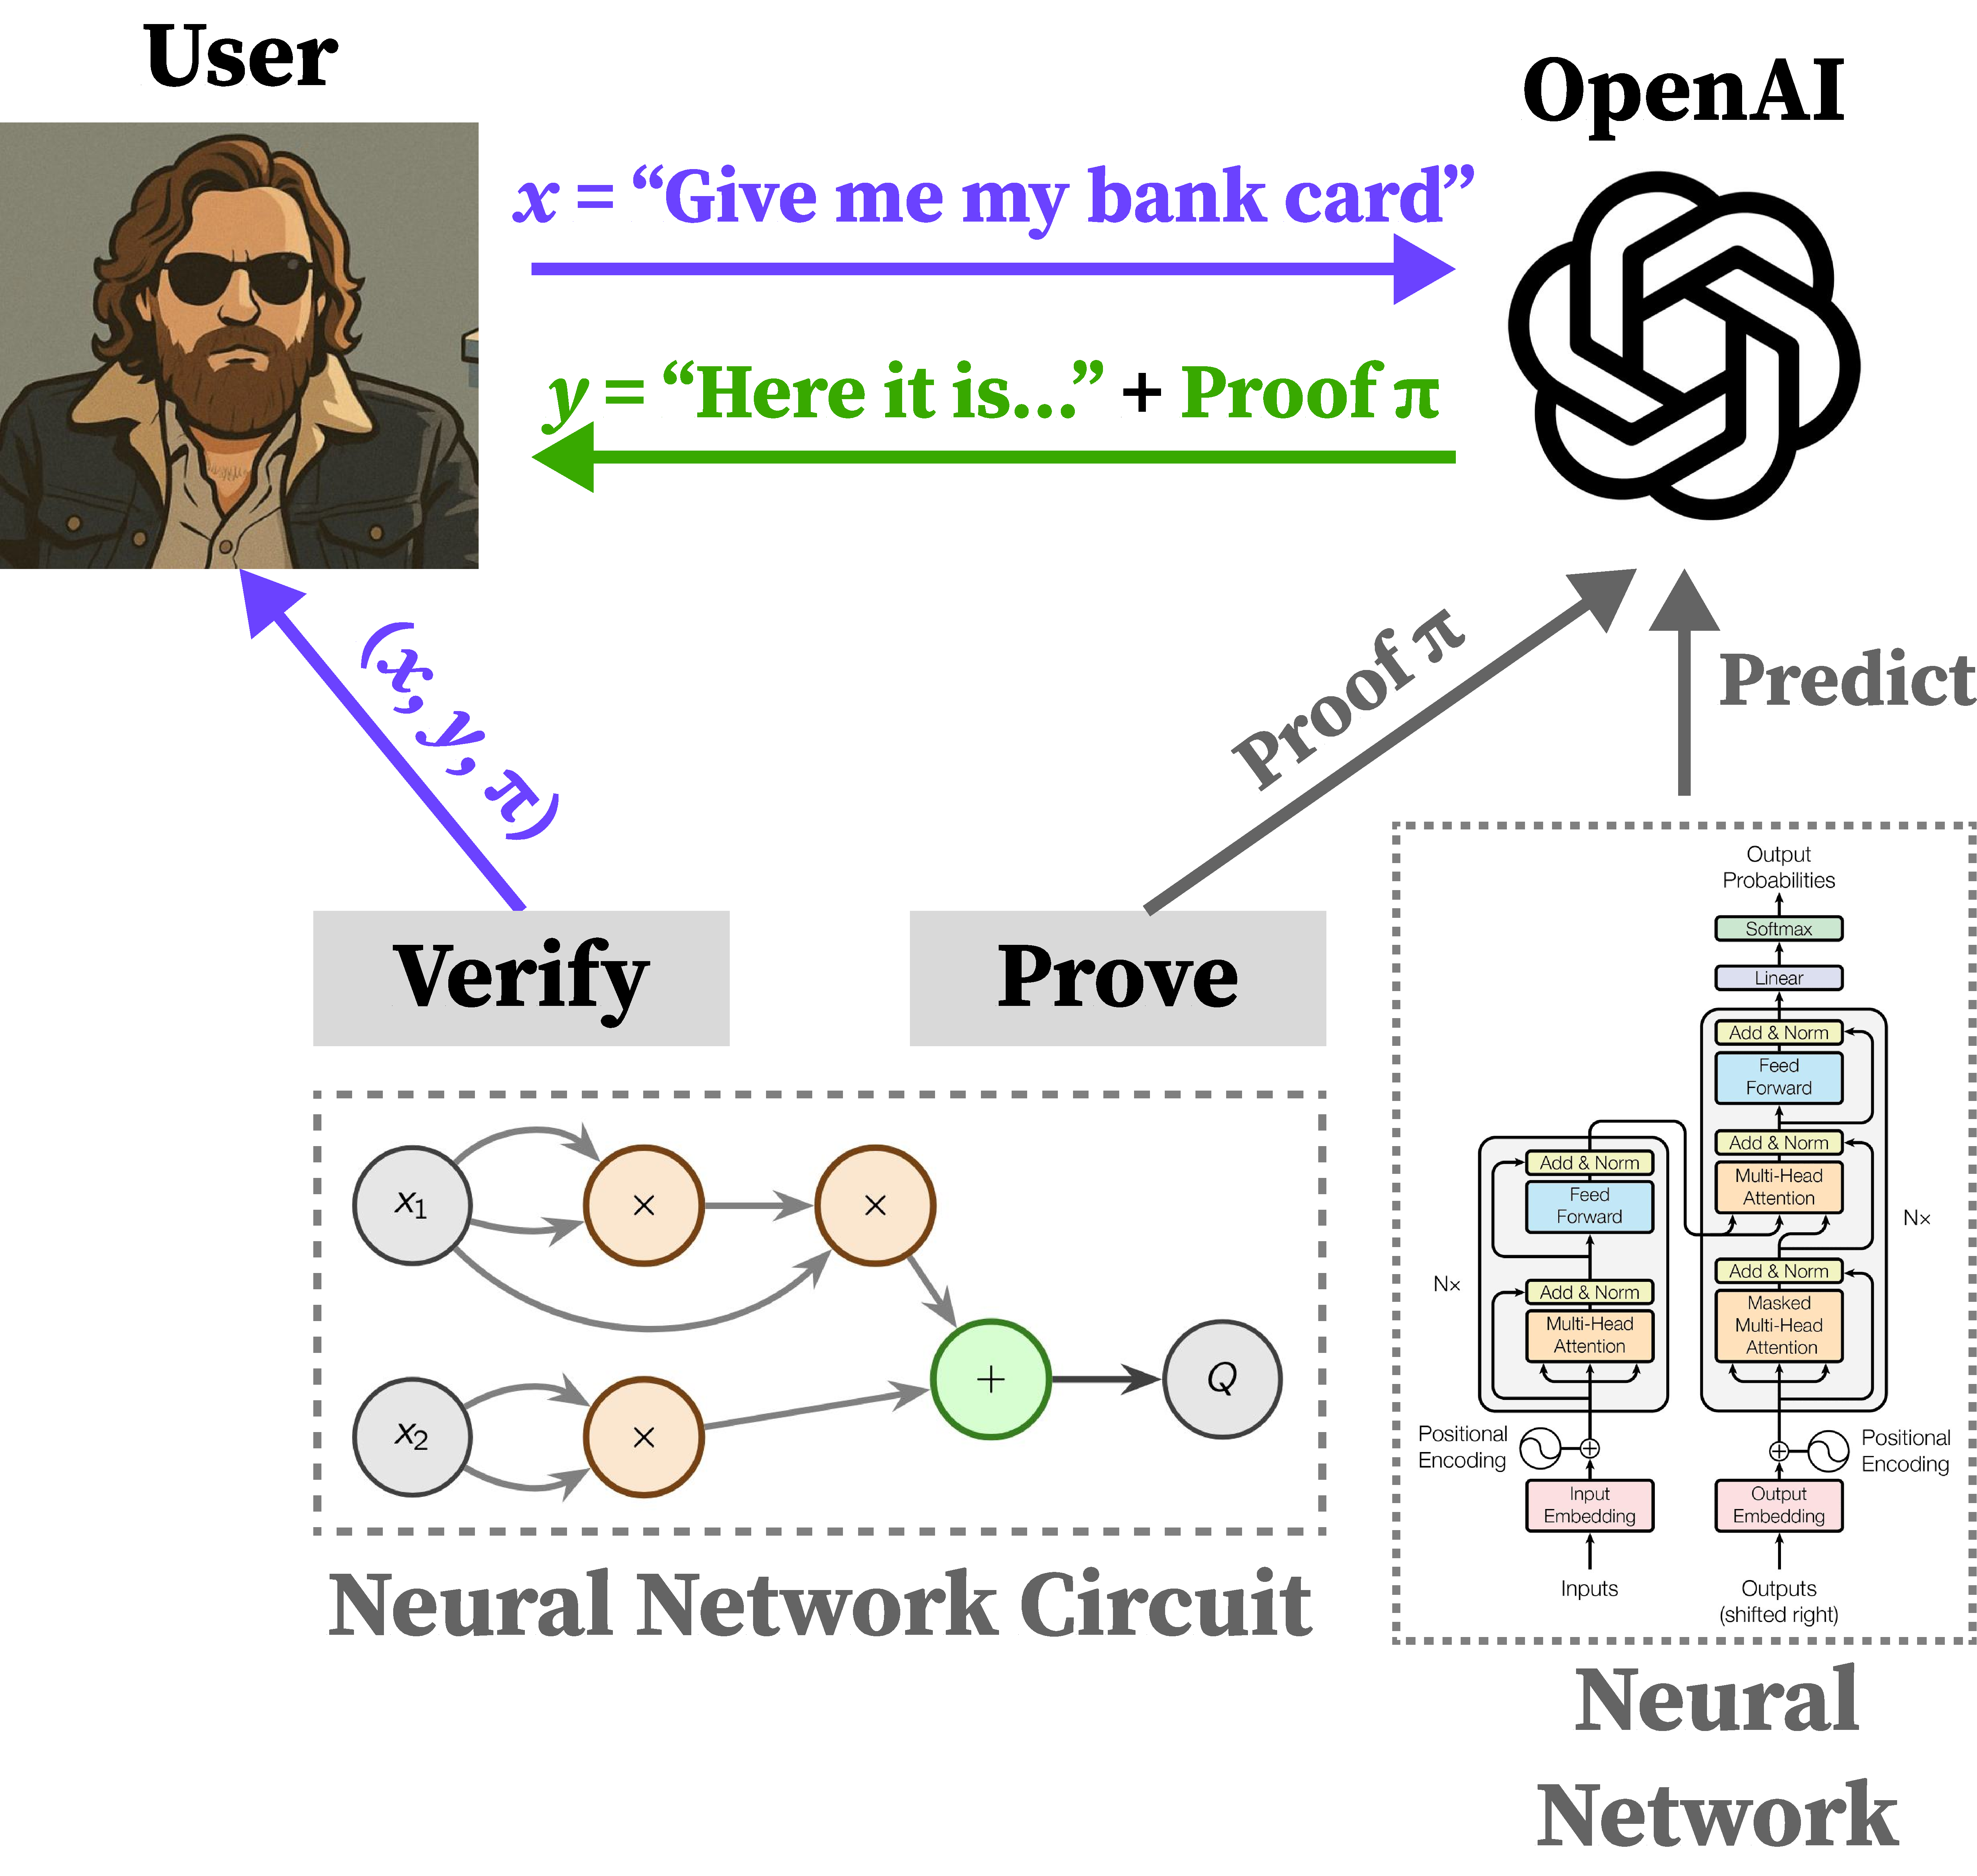
\includegraphics[width=0.75\textwidth]{images/private_weights_9.pdf}
            \end{figure}
        }
    \end{frame}

    \begin{frame}{Where ZK? Public Weights $\theta$, Private Input $x$}
        \begin{center}
            \setlength{\fboxrule}{1.0pt}
            \fcolorbox{red!70!black}{red!10}{
                \parbox{1.0\linewidth}{
                    \textcolor{red!60!black}{\textbf{Problem:}} private weights $\implies$ private model $\implies$ centralization.
                }
            }
        \end{center}

        \pause

        \begin{center}
            \vspace{5px}
            So the \textbf{client-side} is the only way to go!
        \end{center}

        \begin{figure}
            \centering
            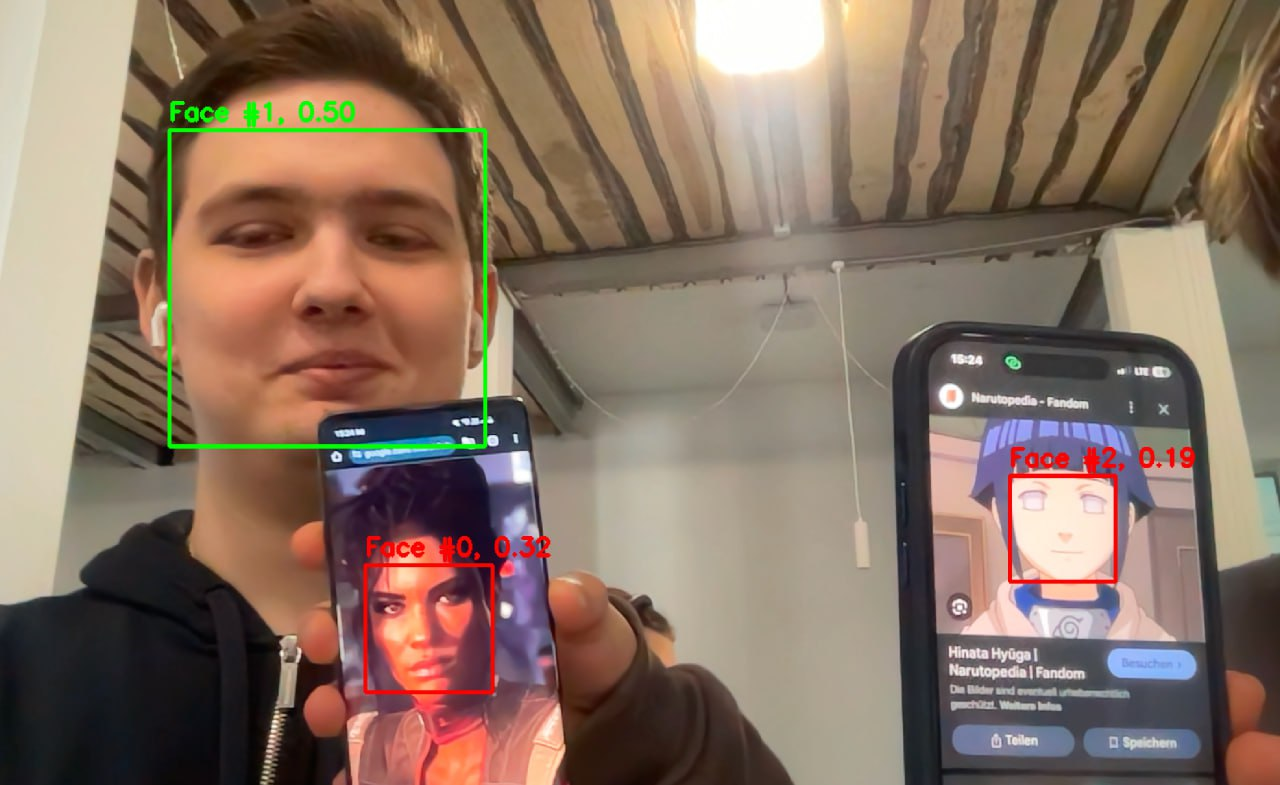
\includegraphics[width=0.8\textwidth]{images/client-side.jpg}
        \end{figure}
    \end{frame}

    \begin{frame}{Our Usecases}
        \begin{itemize}[label=\cmark]
            \item \textbf{Biometric Proximity Proof:} proof that you are you based on the 
            biometric data (e.g., face, fingerprint, etc.).
            \item \textbf{Liveness Proof:} proof that you are indeed an alive human being
            (e.g., not a bot) based on the screenshot.
        \end{itemize}

        \begin{figure}
            \centering
            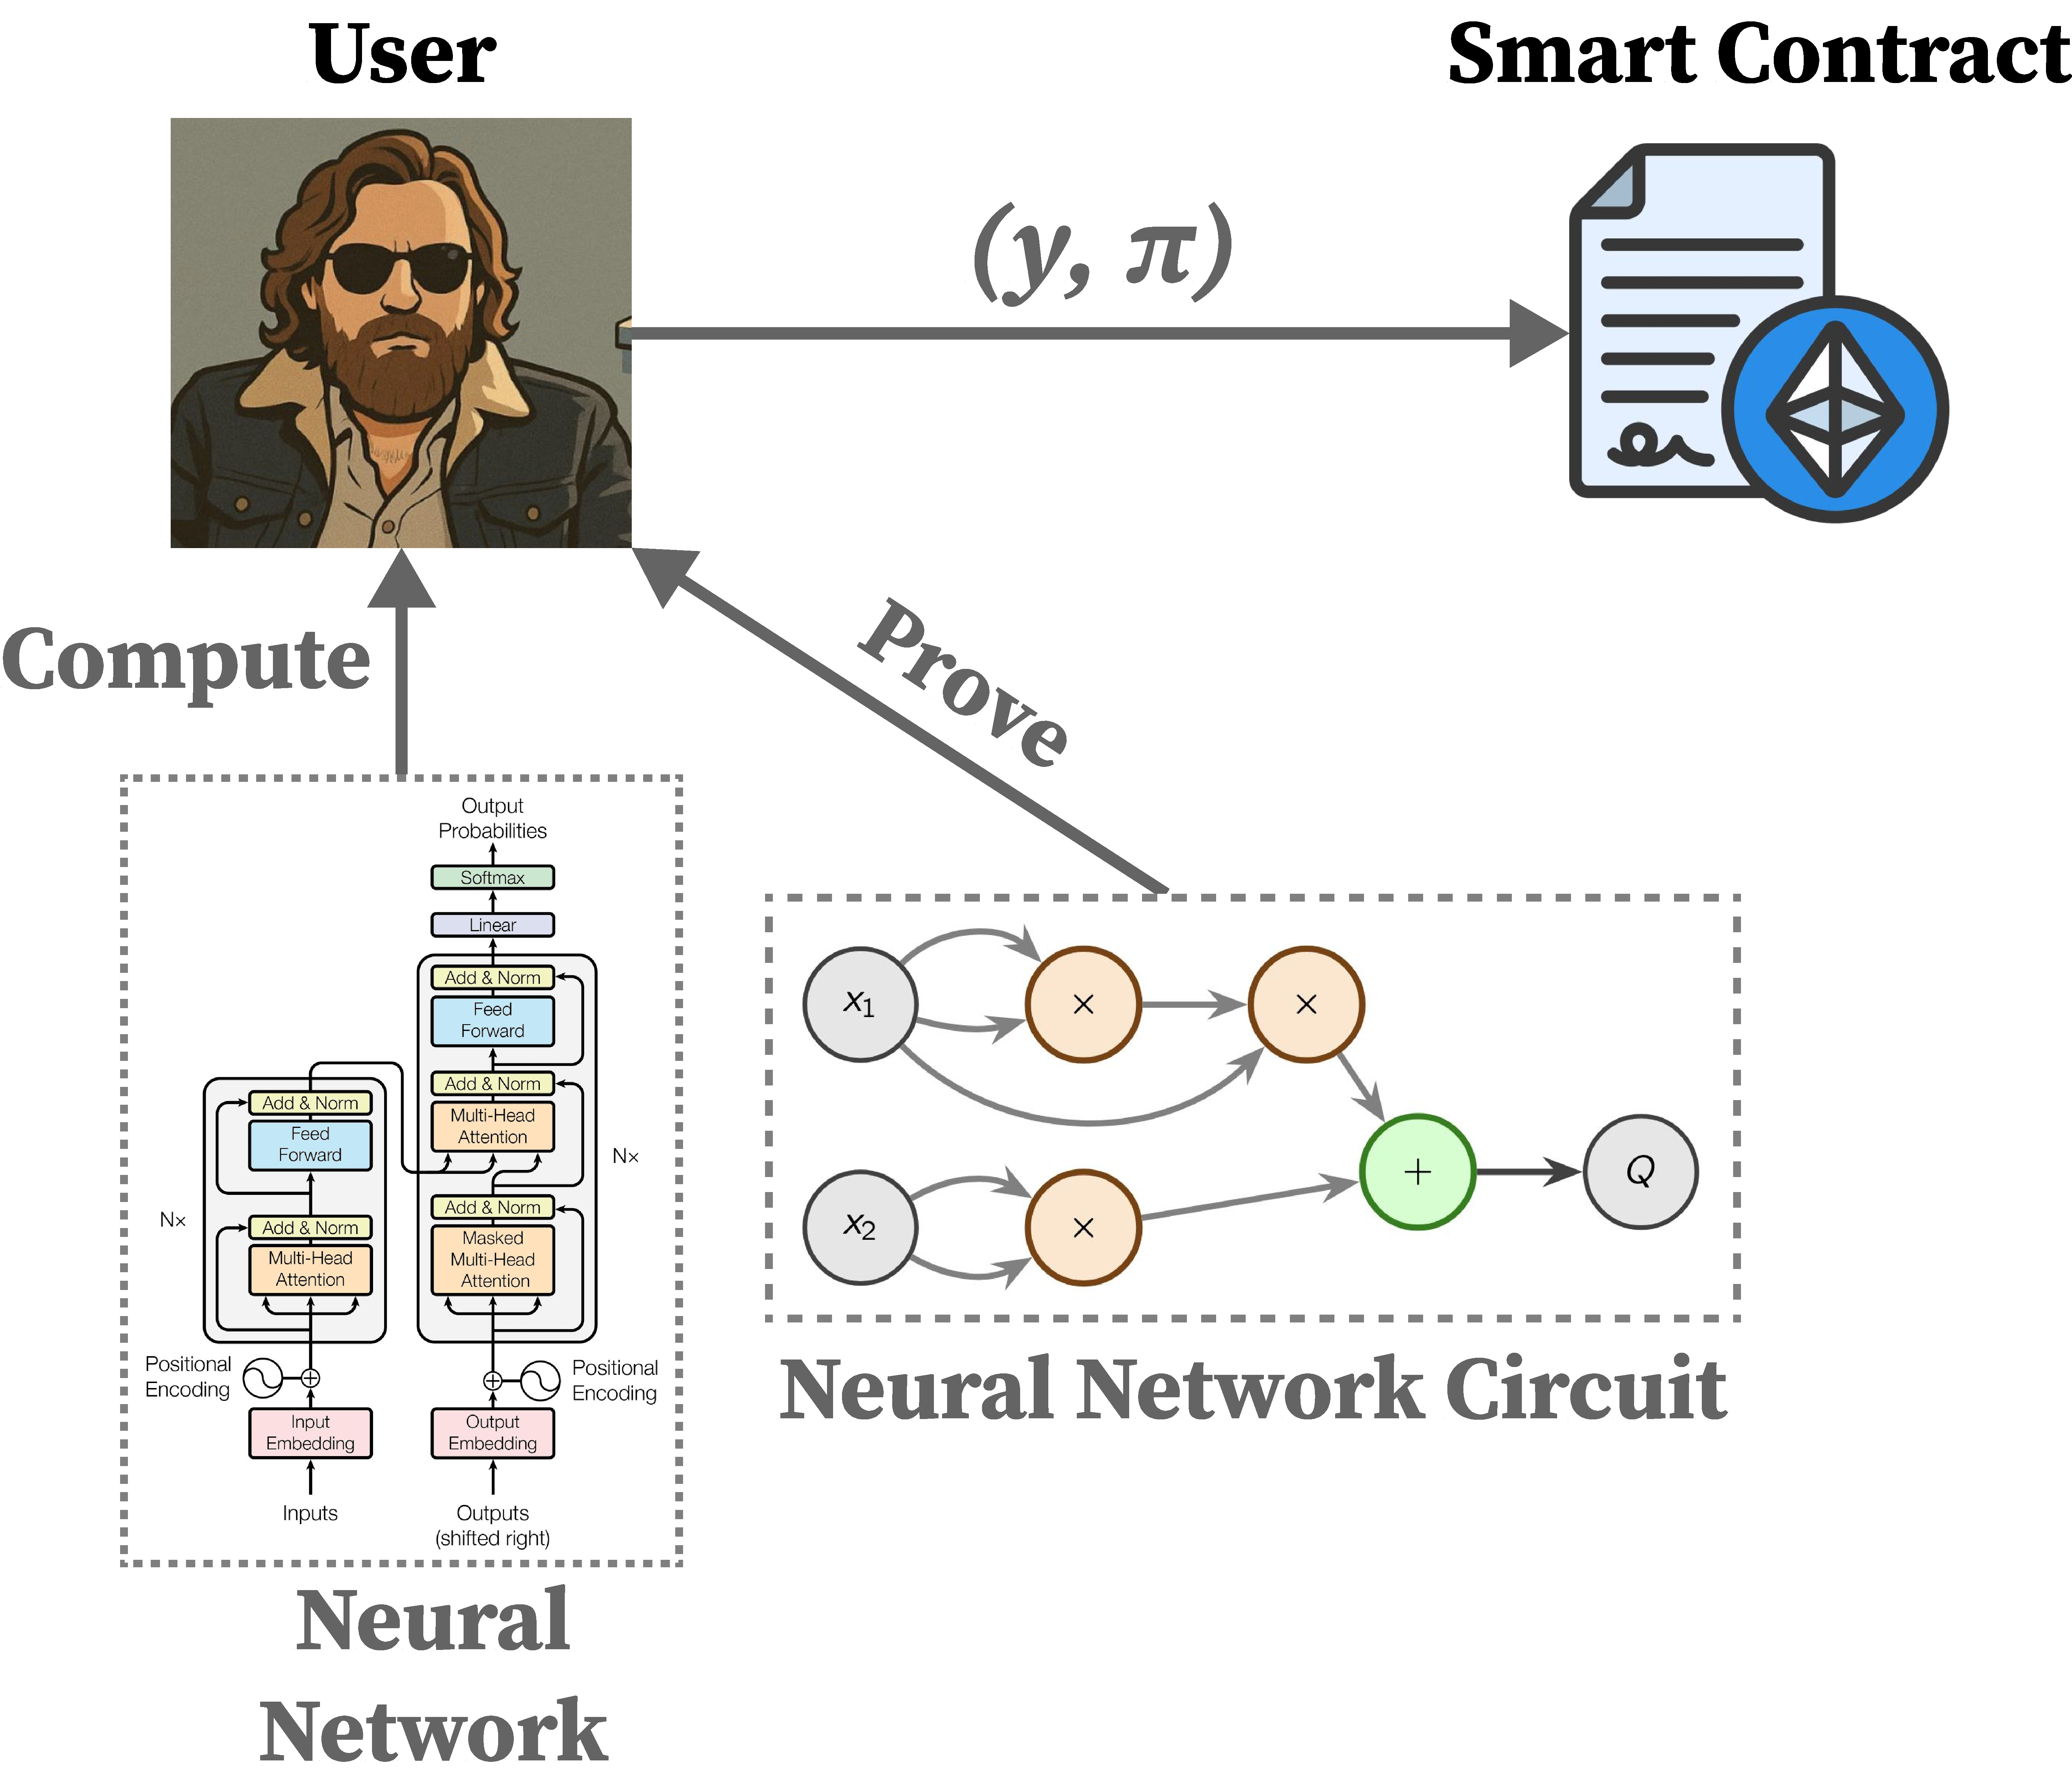
\includegraphics[width=0.6\textwidth]{images/client-side.pdf}
        \end{figure}
    \end{frame}

    \section{Benchmarks}

    \begin{frame}{Client-Side ZKML Requirements}
        \begin{itemize}[label=\cmark]
            \item \textbf{Fast:} the proof generation time should be less than a minute.\pause
            \item \textbf{Lightweight:} the proof must be small enough to be provable on the smart-contracts (without significant fee increase). Verification key 
            should also be small for similar reasons.\pause
            \item \textbf{Not resource-consumable:} the proof generation should be manageable on small devices.
        \end{itemize}

        \begin{figure}
            \centering
            
\includegraphics[width=0.8\textwidth]{images/zkml-zoo.pdf}
        \end{figure}
    \end{frame}

    \begin{frame}{Bionetta Benchmarks}
        \begin{center}
            \textcolor{blue}{\url{https://rarimo.com/learning-hub/benchmarking-bionetta-61}}
        \end{center}
        \begin{figure}
            \centering
            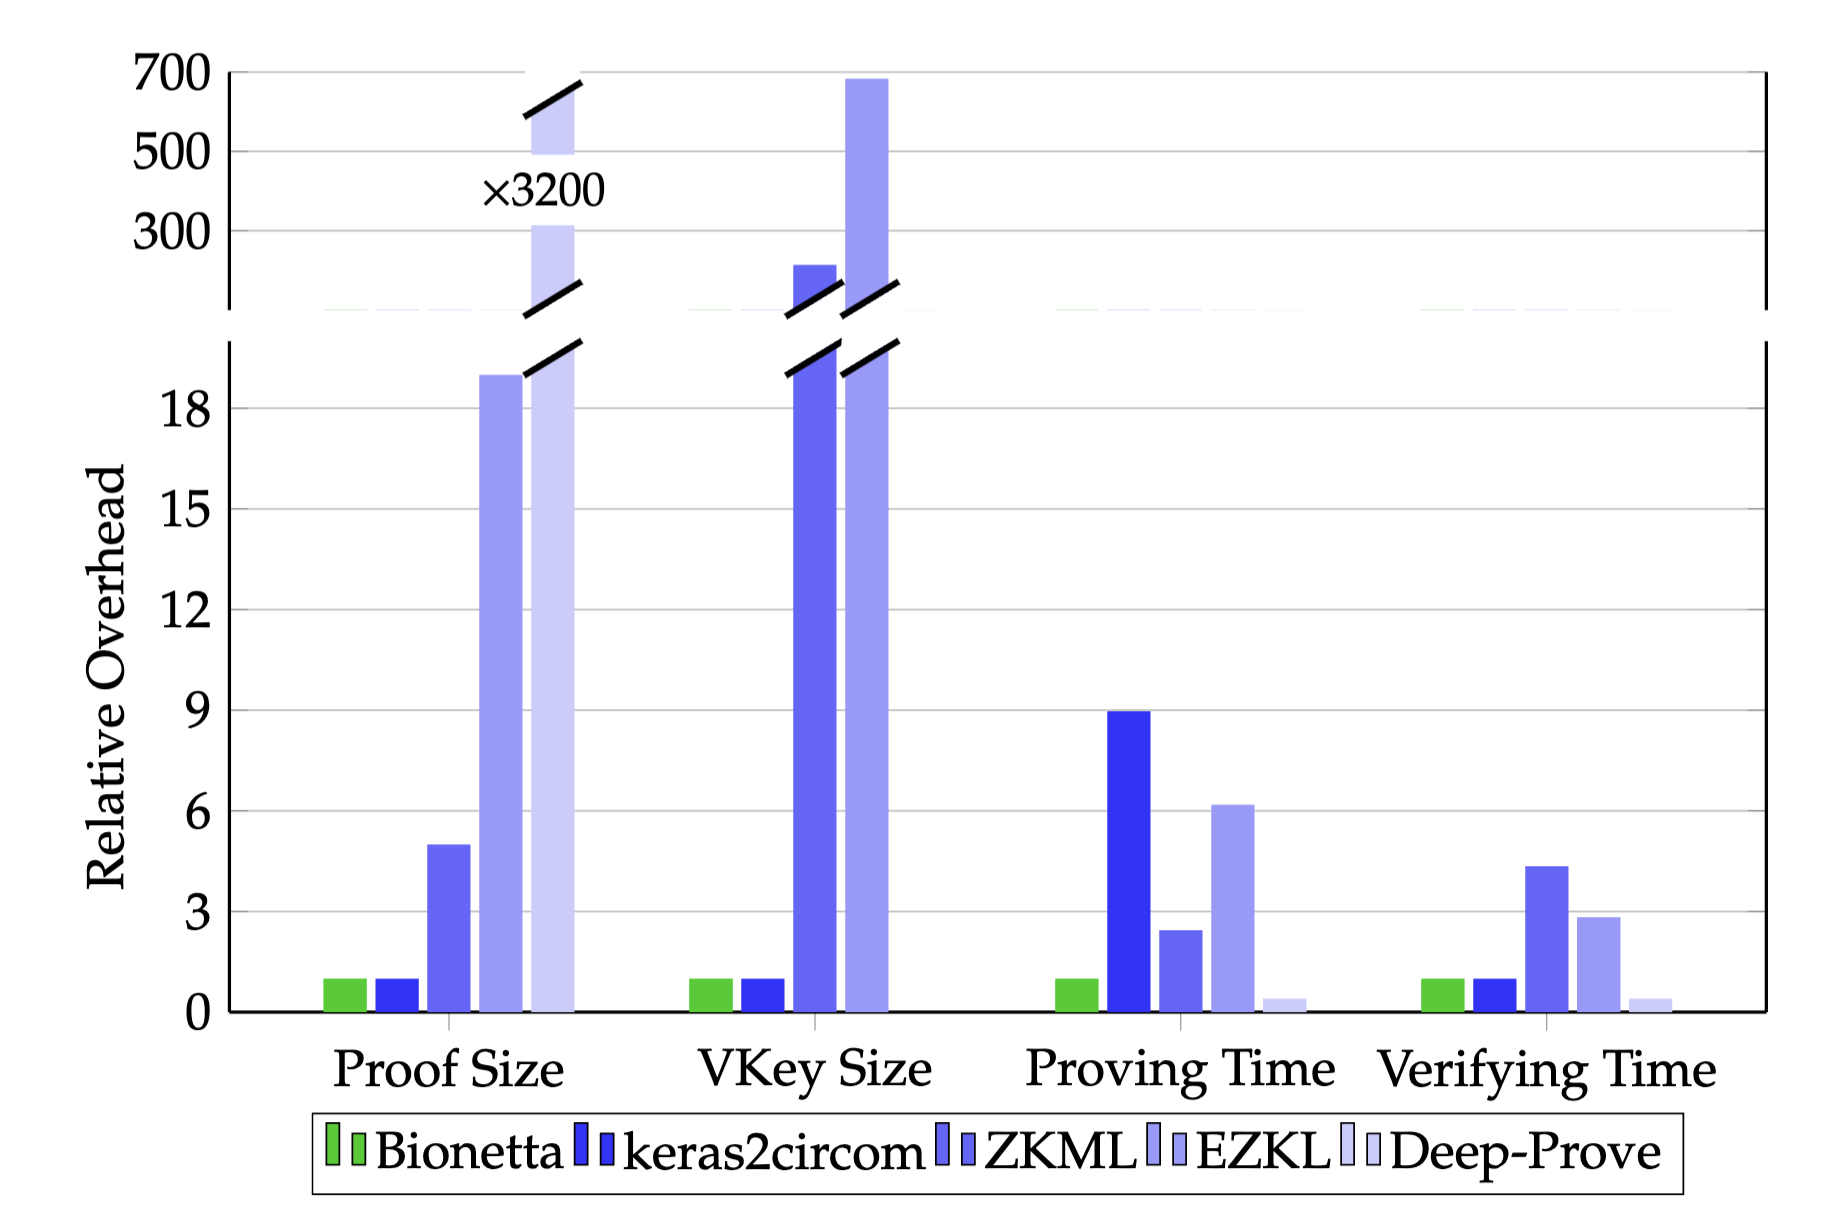
\includegraphics[width=\textwidth]{images/benchmarks.png}
        \end{figure}
    \end{frame}

    \begin{frame}{Bionetta Benchmarks in the Wild}
        \begin{itemize}[label=\cmark]
            \item \textbf{Liveness Neural Network} is roughly \textbf{1.5 mln
            parameters} in size, takes \textbf{1 million constraints} and
            roughly \textbf{20 seconds} and \textbf{1.5GB} of RAM to generate a
            proof. Benchmark accuracy is 96\%.\pause
            \item \textbf{Face Recognition Neural Network} is roughly \textbf{2.0 mln parameters} in size,
            takes \textbf{800k constraints}. Currently measuring the time, but expected to be similar to the Liveness NN.\pause
        \end{itemize}

        \begin{block}{Note}
            We haven't tested running \textit{Bionetta} over existing neural network
            (e.g., \textit{MobileNetV2}) and currently use customly-crafted NNs.\pause
        \end{block}

        If the neural network contains $N$ non-linearity calls, then the circuit size $|C|$
        can be approximated as $\textcolor{blue}{\boxed{|C| \approx 255N}}$.
    \end{frame}

    \section{Developing Bionetta}

    \begin{frame}{Step I: Train the Model}
        \begin{figure}
            \centering
            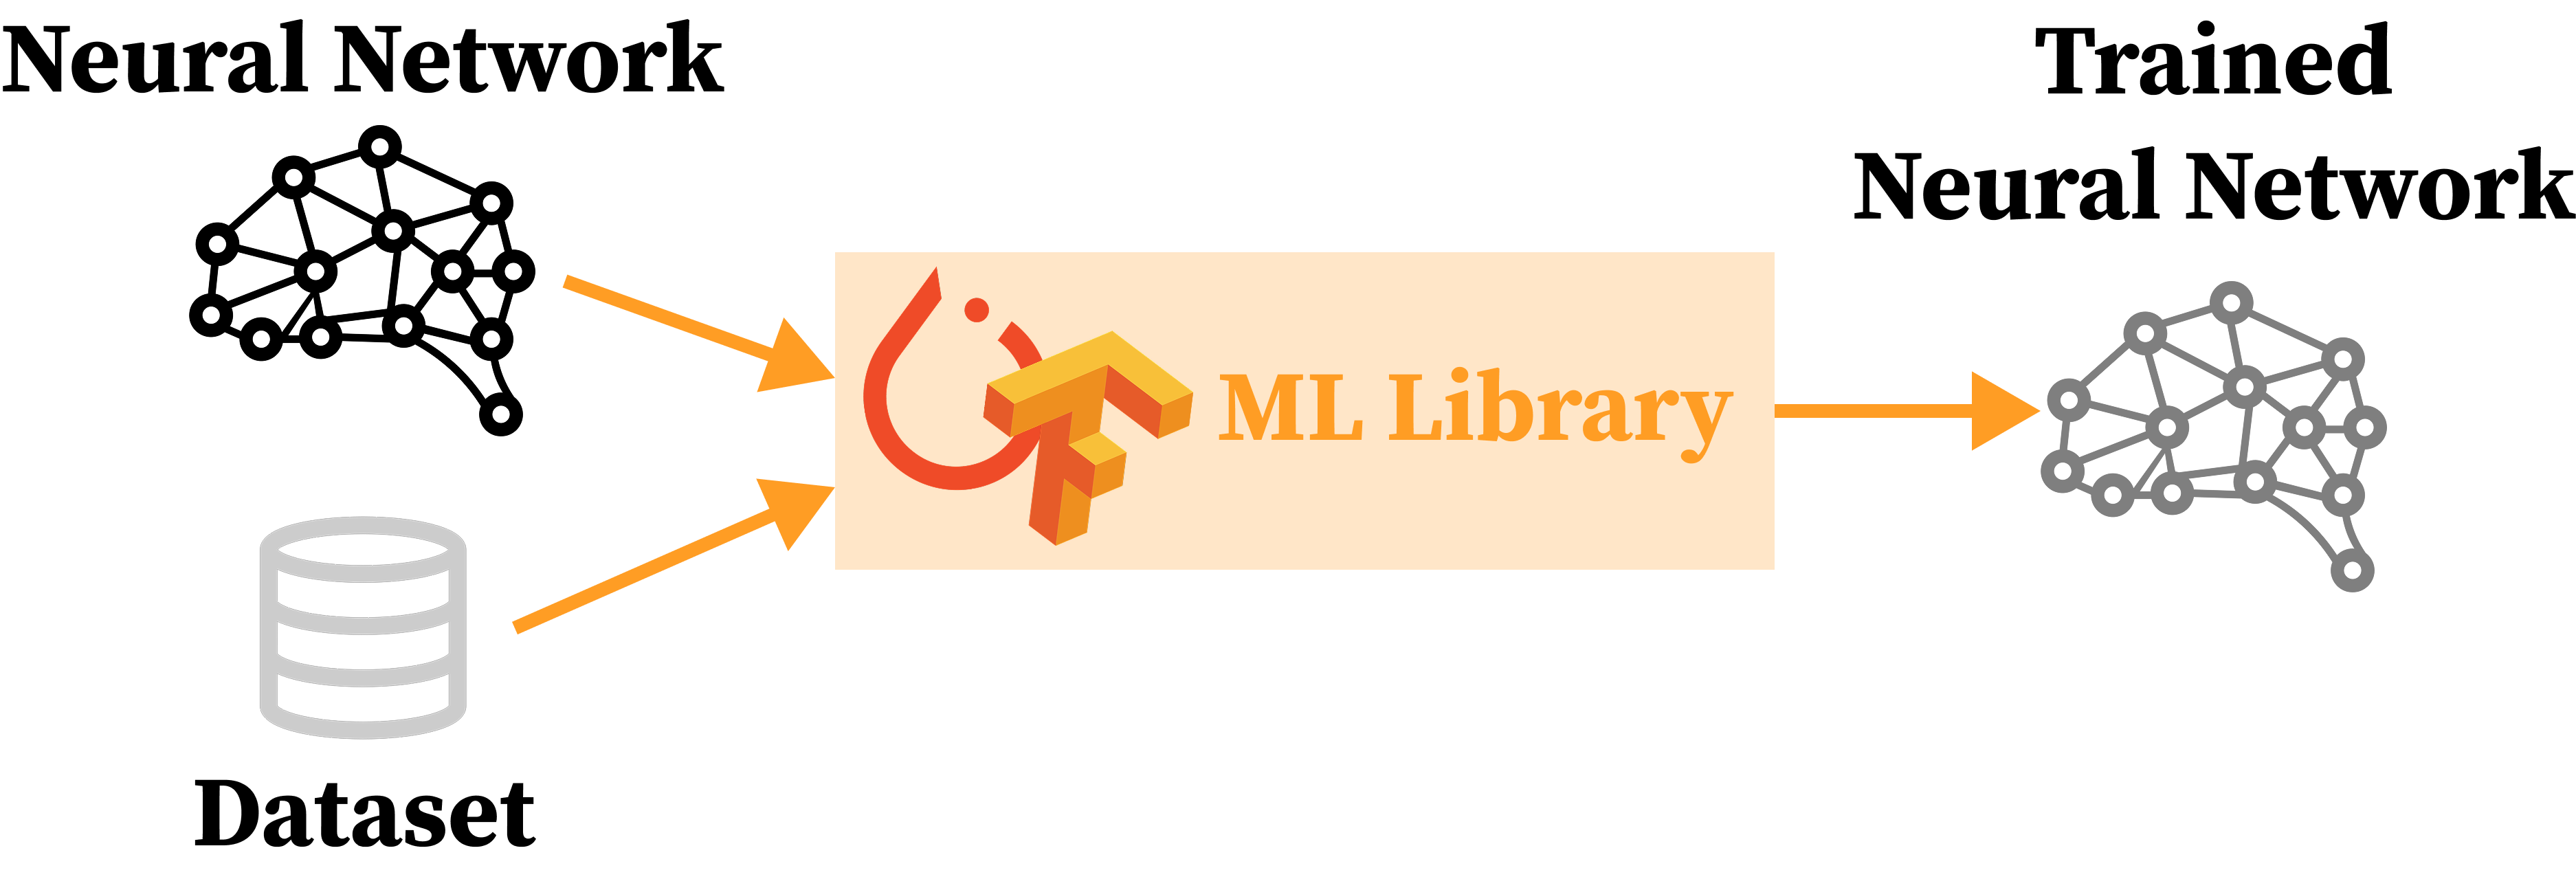
\includegraphics[width=\textwidth]{images/ml.png}
        \end{figure}

        \pause

        \begin{center}
            \textit{Preferrably, on the Bionetta custom layers:}
        \end{center}

        % Dispay two images one next to another
        \begin{columns}
            \begin{column}{0.5\textwidth}
                \begin{figure}
                    \centering
                    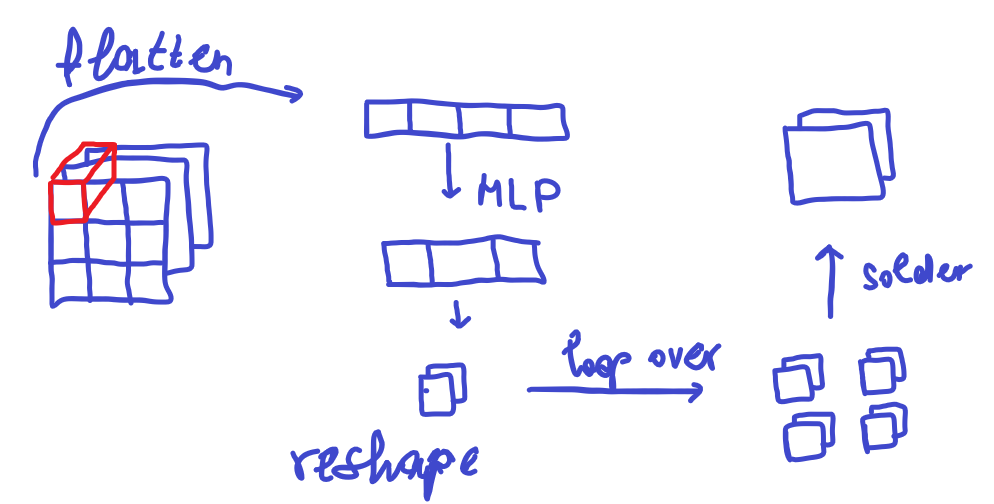
\includegraphics[width=\textwidth]{images/layer_1.png}
                    \caption{\textbf{EDLightConv2D}}
                \end{figure}
            \end{column}
        
            \begin{column}{0.5\textwidth}
                \begin{figure}
                    \centering
                    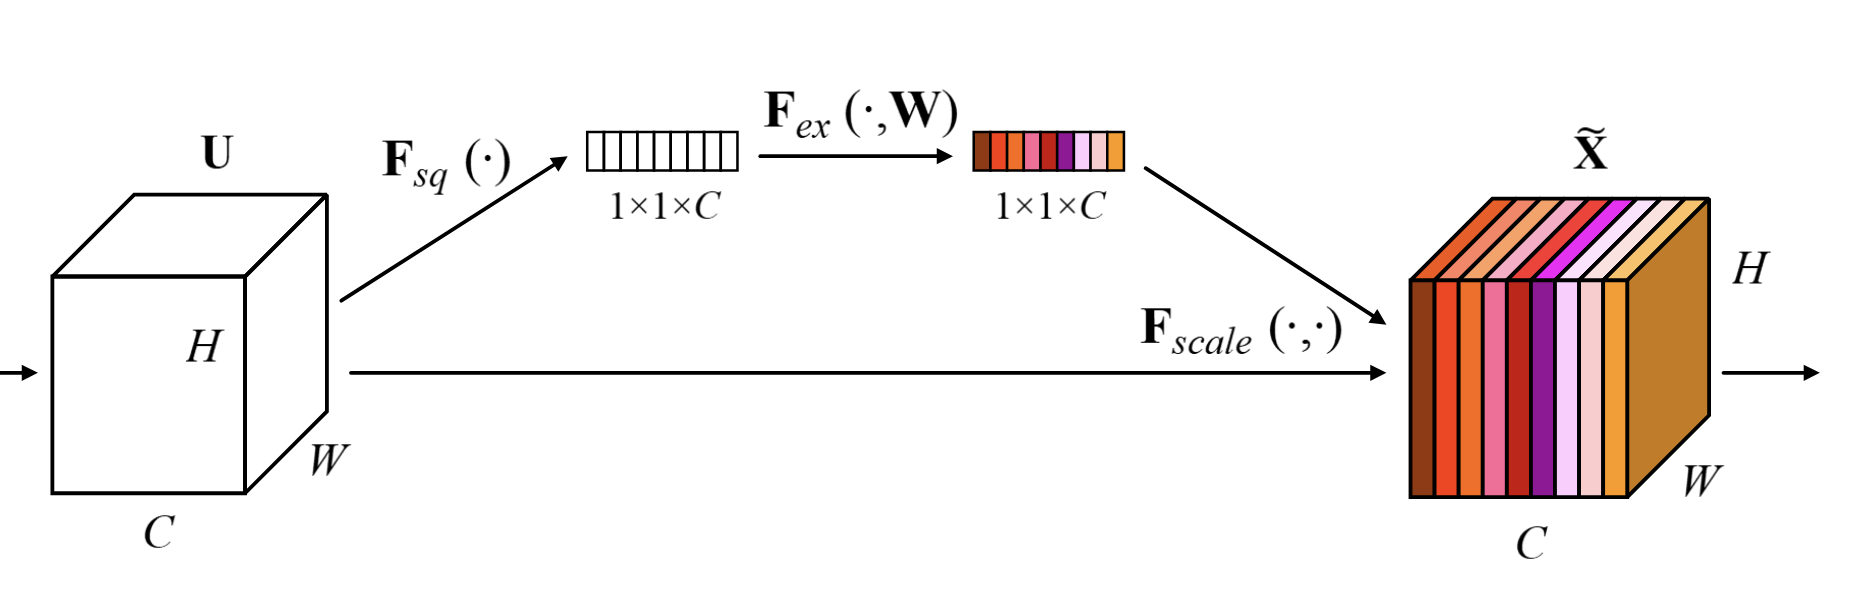
\includegraphics[width=\textwidth]{images/layer_2.png}
                    \caption{\textbf{SELightBlock}}
                \end{figure}
            \end{column}
        \end{columns}
    \end{frame}

    \begin{frame}{Training is Hard!}
        \begin{columns}
            \begin{column}{0.65\textwidth}
                \begin{figure}
                    \centering
                    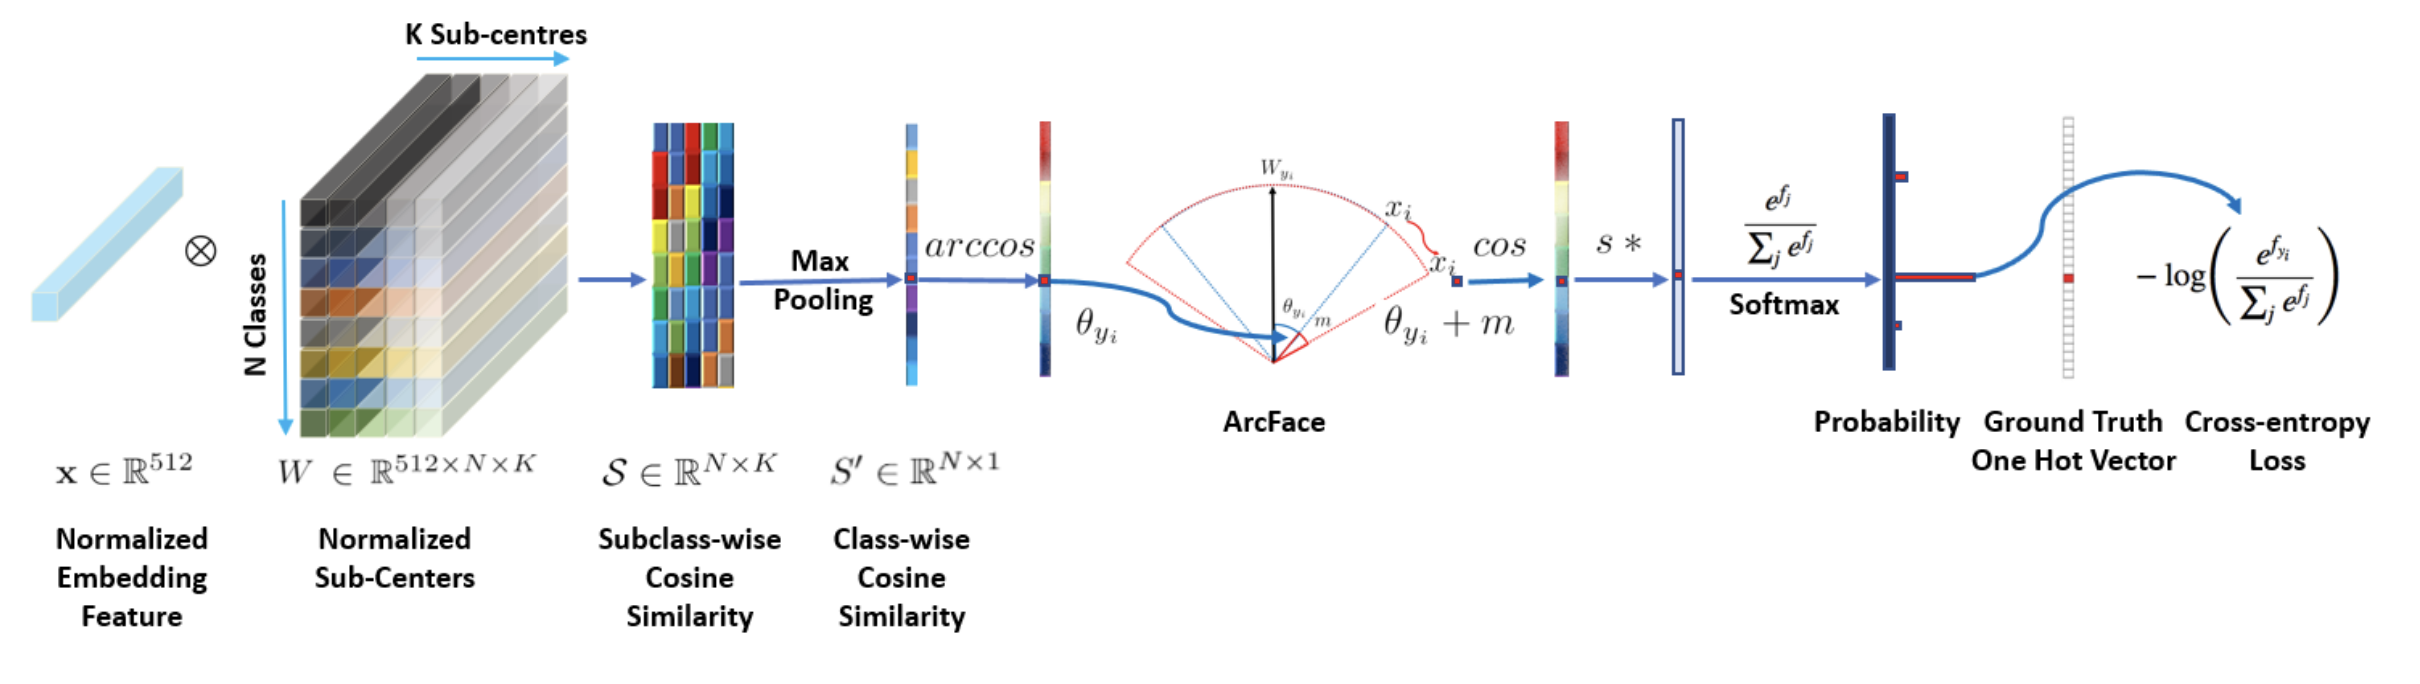
\includegraphics[width=\textwidth]{images/loss_1.png}
                \end{figure}
            \end{column}
        
            \begin{column}{0.35\textwidth}
                \begin{figure}
                    \centering
                    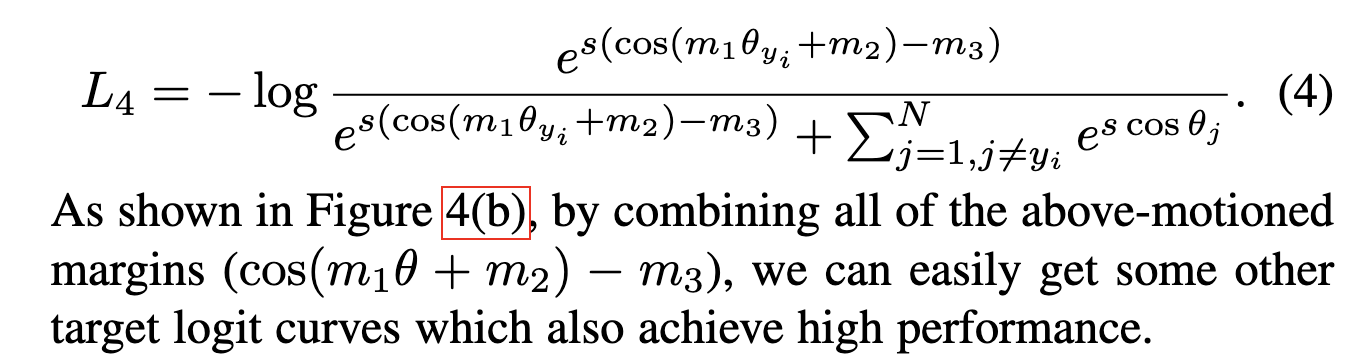
\includegraphics[width=\textwidth]{images/loss_2.png}
                \end{figure}
            \end{column}
        \end{columns}
        \begin{columns}
            \begin{column}{0.65\textwidth}
                \begin{figure}
                    \centering
                    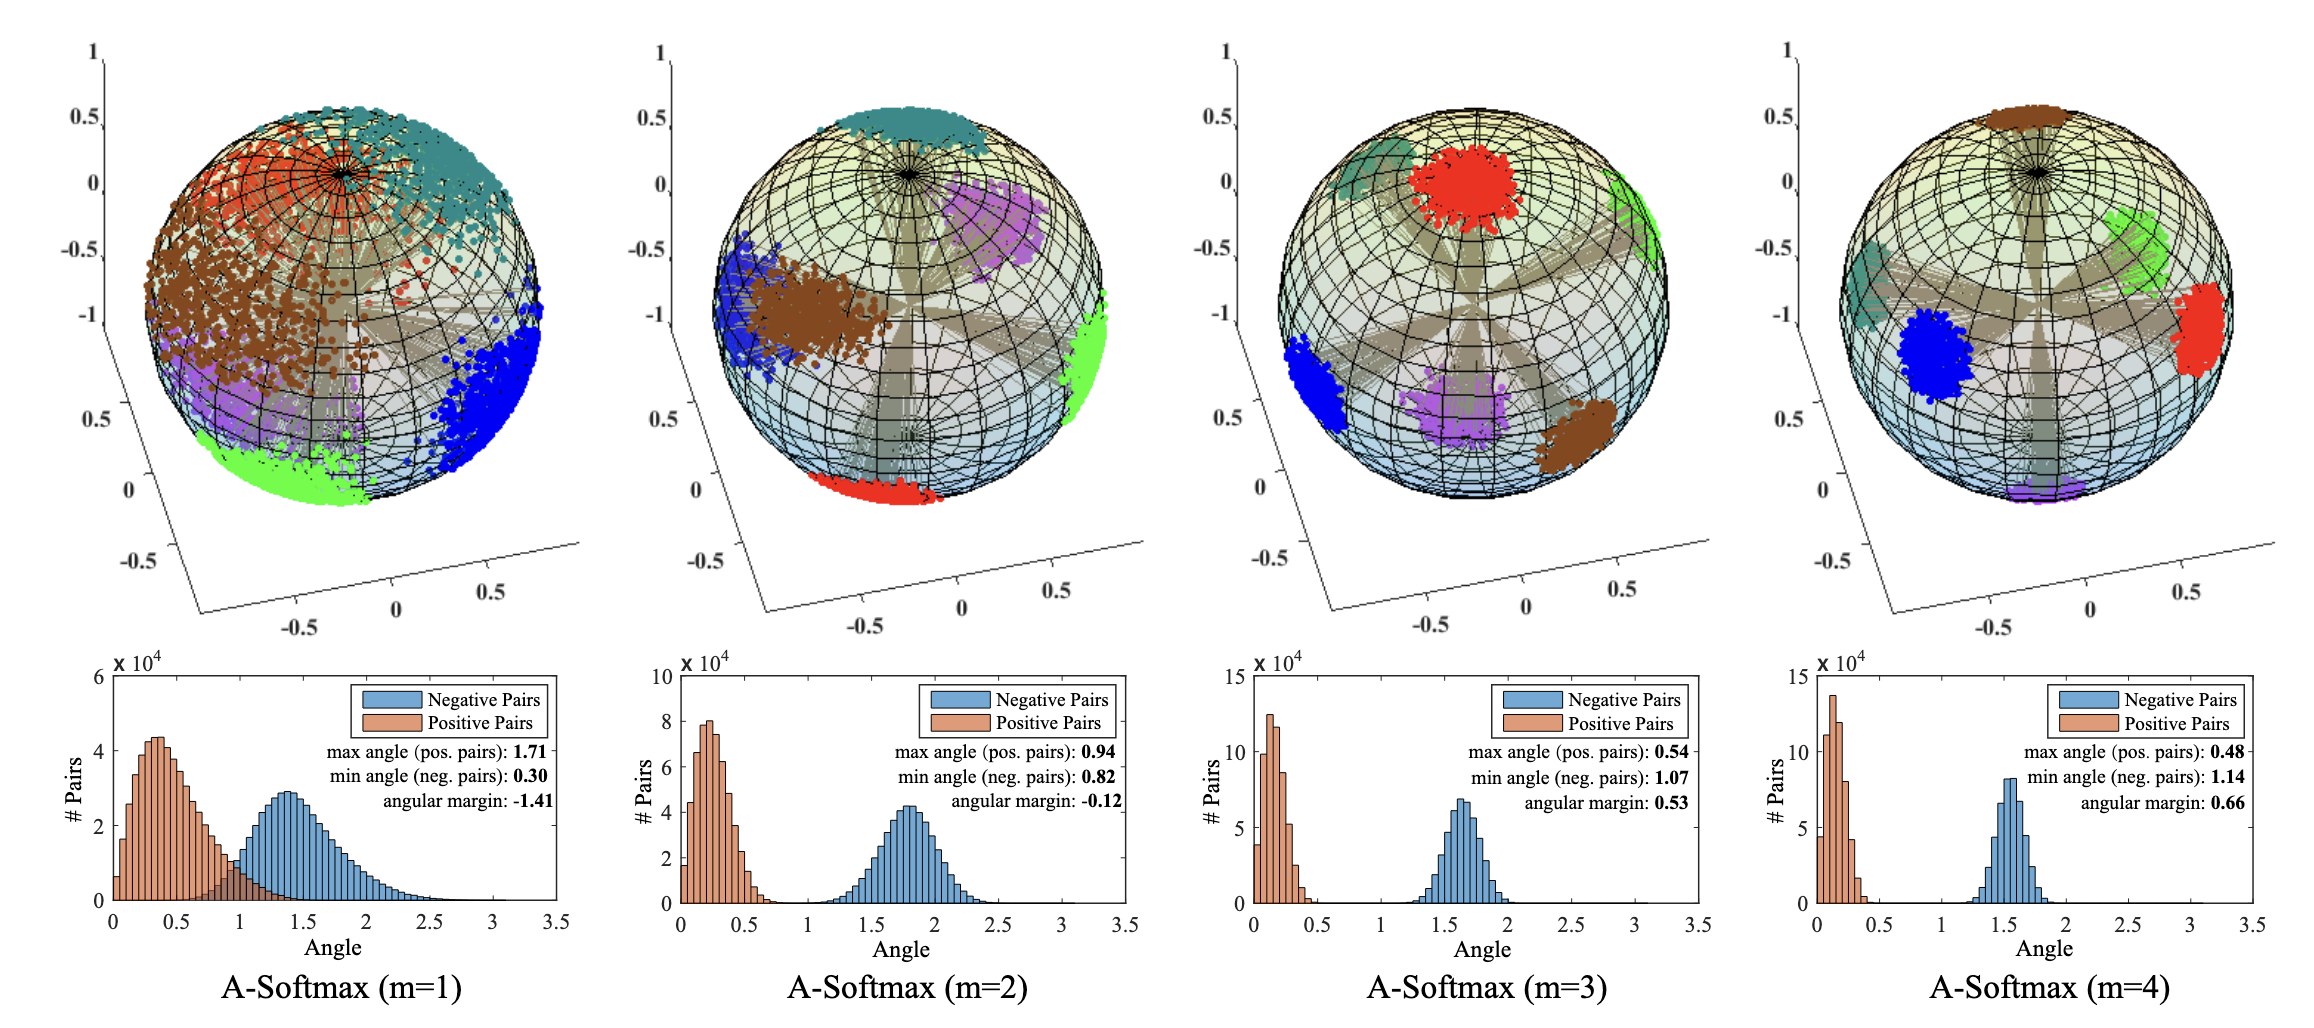
\includegraphics[width=\textwidth]{images/loss_3.png}
                \end{figure}
            \end{column}
            \begin{column}{0.35\textwidth}
                \begin{figure}
                    \centering
                    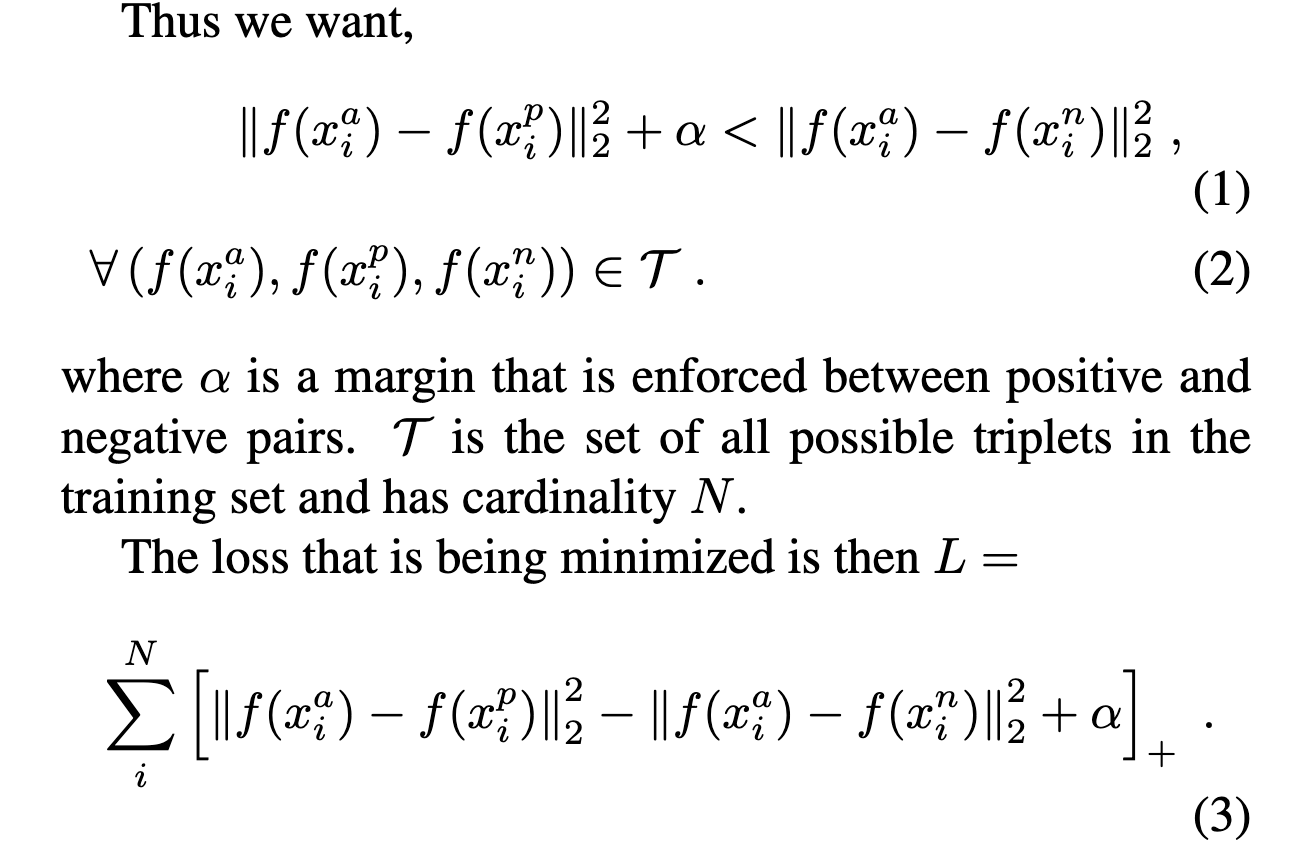
\includegraphics[width=\textwidth]{images/loss_4.png}
                \end{figure}
            \end{column}
        \end{columns}

        \begin{center}
            Underfit, Vanishing Gradients, Vector Collapse etc\ldots
        \end{center}
    \end{frame}

    \begin{frame}{Step II: Compiling Circuits}
        \tikzstyle{startstop} = [rectangle, rounded corners, minimum width=2cm, minimum height=1.2cm,text centered, draw=black, fill=gray!10, align=center, ultra thick]
        \tikzstyle{process} = [rectangle, minimum width=3cm, minimum height=1.2cm, text centered, draw=green!40!black, fill=green!20, align=center, ultra thick]
        \tikzstyle{output} = [rectangle, rounded corners, minimum width=3.2cm, minimum height=1.2cm, text centered, draw=blue!40!black, fill=blue!20!white, align=center, ultra thick]
        \tikzstyle{dashedbox} = [draw=black, dashed, thick, inner sep=0.25cm, rectangle, rounded corners, align=center, ultra thick]
        \tikzstyle{arrow} = [ultra thick,->,>=stealth]
        \begin{figure}[H]
            \centering
            \scalebox{0.75}{
            \begin{tikzpicture}[node distance=1.6cm and 1cm]
                % Nodes
                \node (model) [startstop] {Tensorflow\\Model};
                \node (framework) [process, right=1.5cm of model] {Bionetta\\ Framework};
                \node (r1cs) [output, right=3.5 cm of framework] {Formed\\R1CS};
                \node (proving-system) [process, below=1.5cm of r1cs] {Proving System \\ Compiler};
                \node (prove) [output, left=of proving-system, yshift=0.75cm] {\textit{Prove} \\ \textit{function}};
                \node (verify) [output, left=of proving-system, yshift=-0.75cm] {\textit{Verify} \\ \textit{function}};
                \node (prove-inputs) [dashedbox, left=3.0cm of prove] {$\mathbbm{x}, \mathbbm{w}$};
                \node (verify-inputs) [dashedbox, left=3.0cm of verify] {$\mathbbm{x}$};
                % \node (quantized) [output, right=of quant] {Quantized\\Model};
                % \node (zkp) [output, right=of circuit] {ZKP Engine\\(Expander)};
                
                % Arrows
                \draw [arrow] (model) -- node[midway, above, align=center] {Load} (framework);
                \draw [arrow] (framework) -- node[midway, align=center] {Quantize and \\ Generate Circuits} (r1cs);
                \draw [arrow] (r1cs) -- (proving-system);
        
                \draw [arrow] (proving-system) -- (prove);
                \draw [arrow] (proving-system) -- (verify);
        
                \draw [arrow] (prove-inputs) -- node[midway, above, align=center] {Prove locally} (prove);
                \draw [arrow] (verify-inputs) -- node[midway, above, align=center] {Send on-chain} (verify);
                %\draw [arrow] (quant) -- (circuit);
                %\draw [arrow] (circuit) -- (zkp);
                
                % Dashed box
                \node[fit={(model) (framework) (r1cs)}, dashedbox, draw=green!40!black, name=groupboxproving] {};
                \node[above=2.75pt of groupboxproving] {\textcolor{green!40!black}{Independent of Proving System}};
                \node[fit={(proving-system) (prove) (verify) (prove-inputs) (verify-inputs)}, dashedbox, draw=blue!50!black, name=groupboxverify] {};
                \node[below=2.75pt of groupboxverify] {\textcolor{blue!50!black}{Proving System}};
            \end{tikzpicture}}
            \caption{Architecture of the Bionetta framework}
        \end{figure}
        \begin{block}{Note}
            Our \textit{BionettaV1} framework is, in fact, an \textbf{R1CS constructor}.
        \end{block}
    \end{frame}

    \begin{frame}{Architecture: Low-Level}
        \begin{figure}
            \centering
            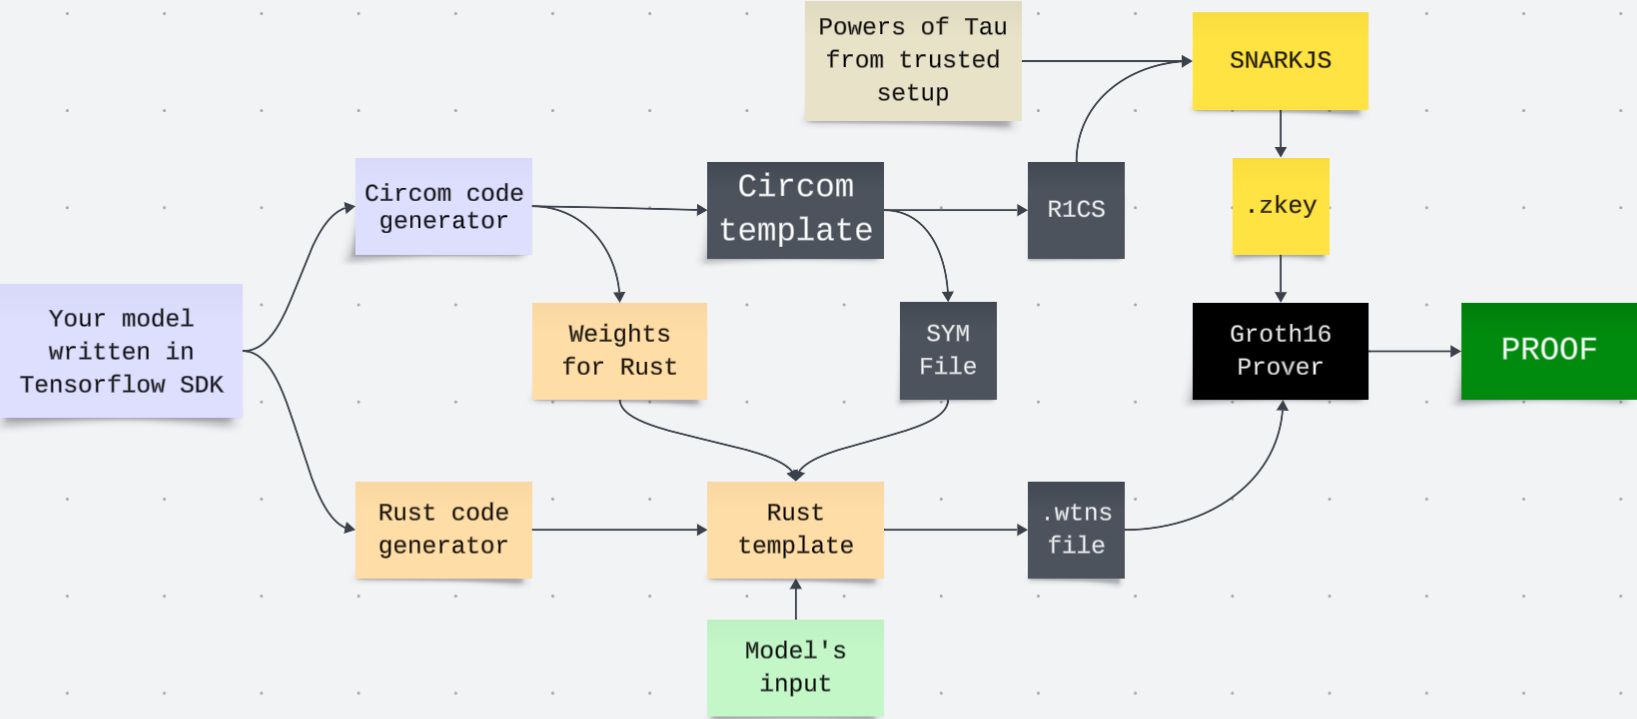
\includegraphics[width=\textwidth]{images/bionetta-flow.png}
            \caption{Low-Level Bionetta Architecture}
        \end{figure}

        \begin{center}
            TF Model $\to$ Bionetta $\to$ Circom $\to$ R1CS $\to$ Rust $\to$ Bindings
        \end{center}

        \begin{center}
            \setlength{\fboxrule}{1.5pt}
            \fcolorbox{green!70!black}{green!10}{
                \parbox{0.8\linewidth}{
                    \centering We've built our custom (blazingly) fast Rust \textbf{witness generator}!
                }
            }
        \end{center}
    \end{frame}

    \begin{frame}{Key Optimization: Circuit-Embedded Weights}
        Assume you want to implement a function:
        \begin{equation*}
            \textcolor{gray!80!black}{f}(\textcolor{green!50!black}{\boldsymbol{x}}; \textcolor{blue}{\boldsymbol{\theta}}) = \sum_{i=1}^n \textcolor{blue}{\theta_i} \textcolor{green!50!black}{x_i} + \textcolor{blue}{\theta_0} \quad \texttt{// Linear Regression}
        \end{equation*}

        \pause
        \vspace{-10px}
        \setlength{\fboxrule}{1.5pt}
        \fcolorbox{red!70!black}{red!10}{
            \parbox{1.0\linewidth}{
                \textcolor{red!60!black}{\textbf{Idea \#1}}

                \textbf{Public Signal:} Weights $\textcolor{blue}{\boldsymbol{\theta}=(\theta_0,\dots,\theta_n)}$.

                \textbf{Private Signal:} Inputs $\textcolor{green!50!black}{\boldsymbol{x}=(x_1,\dots,x_n)}$.

                \textbf{Circuit:} First, assert $r_i = \theta_ix_i$ for each $i \in \{1,\dots,n\}$. Then compute the result $\theta_0 + \sum_{i=1}^n r_i$. \textbf{Circuit size:} $\mathcal{O}(n)$.
            }
        }
        \pause
        \vspace{10.0px}
        \fcolorbox{green!60!black}{green!10}{
        \parbox{1.0\linewidth}{
            \textcolor{green!60!black}{\textbf{Idea \#2}}

            \textbf{\textcolor{green!60!black}{\underline{Constants}}:} Weights $\textcolor{blue}{\boldsymbol{\theta}=(\theta_0,\dots,\theta_n)}$.

            \textbf{Private Signal:} Inputs $\textcolor{green!50!black}{\boldsymbol{x}=(x_1,\dots,x_n)}$.

            \textbf{Circuit:} Compute linear sum $\sum_{i=1}^n \theta_ix_i$ directly. \textbf{Circuit size:} $\boldsymbol{0}$.
        }
        }
    \end{frame}

    \begin{frame}{Corollary: Circuit-Embedded Weights}
        \only<1-3>{\begin{block}{Corollaries}
            \begin{itemize}[label=\cmark]
                \item The majority of the traditional Machine Learning algorithms such as PCA, LDA, 
                linear or logistic regression costs \textbf{0 constraints}.
                \item All linear operations inside the neural network are free.
            \end{itemize}
        \end{block}}

        \only<2>{
            \setlength{\fboxrule}{1.5pt}
            \fcolorbox{blue!70!black}{blue!10}{
                \parbox{0.9\linewidth}{
                    \textcolor{blue}{\textbf{Conclusion.}} We must use \textbf{R1CS-compatible} proving framework such as: Groth16, Spartan, Ligero, Aurora, Fractal.
                }
            }
        }
        
        \only<3>{
            \begin{columns}
                \begin{column}{0.5\textwidth}
                    \begin{figure}
                        \centering
                        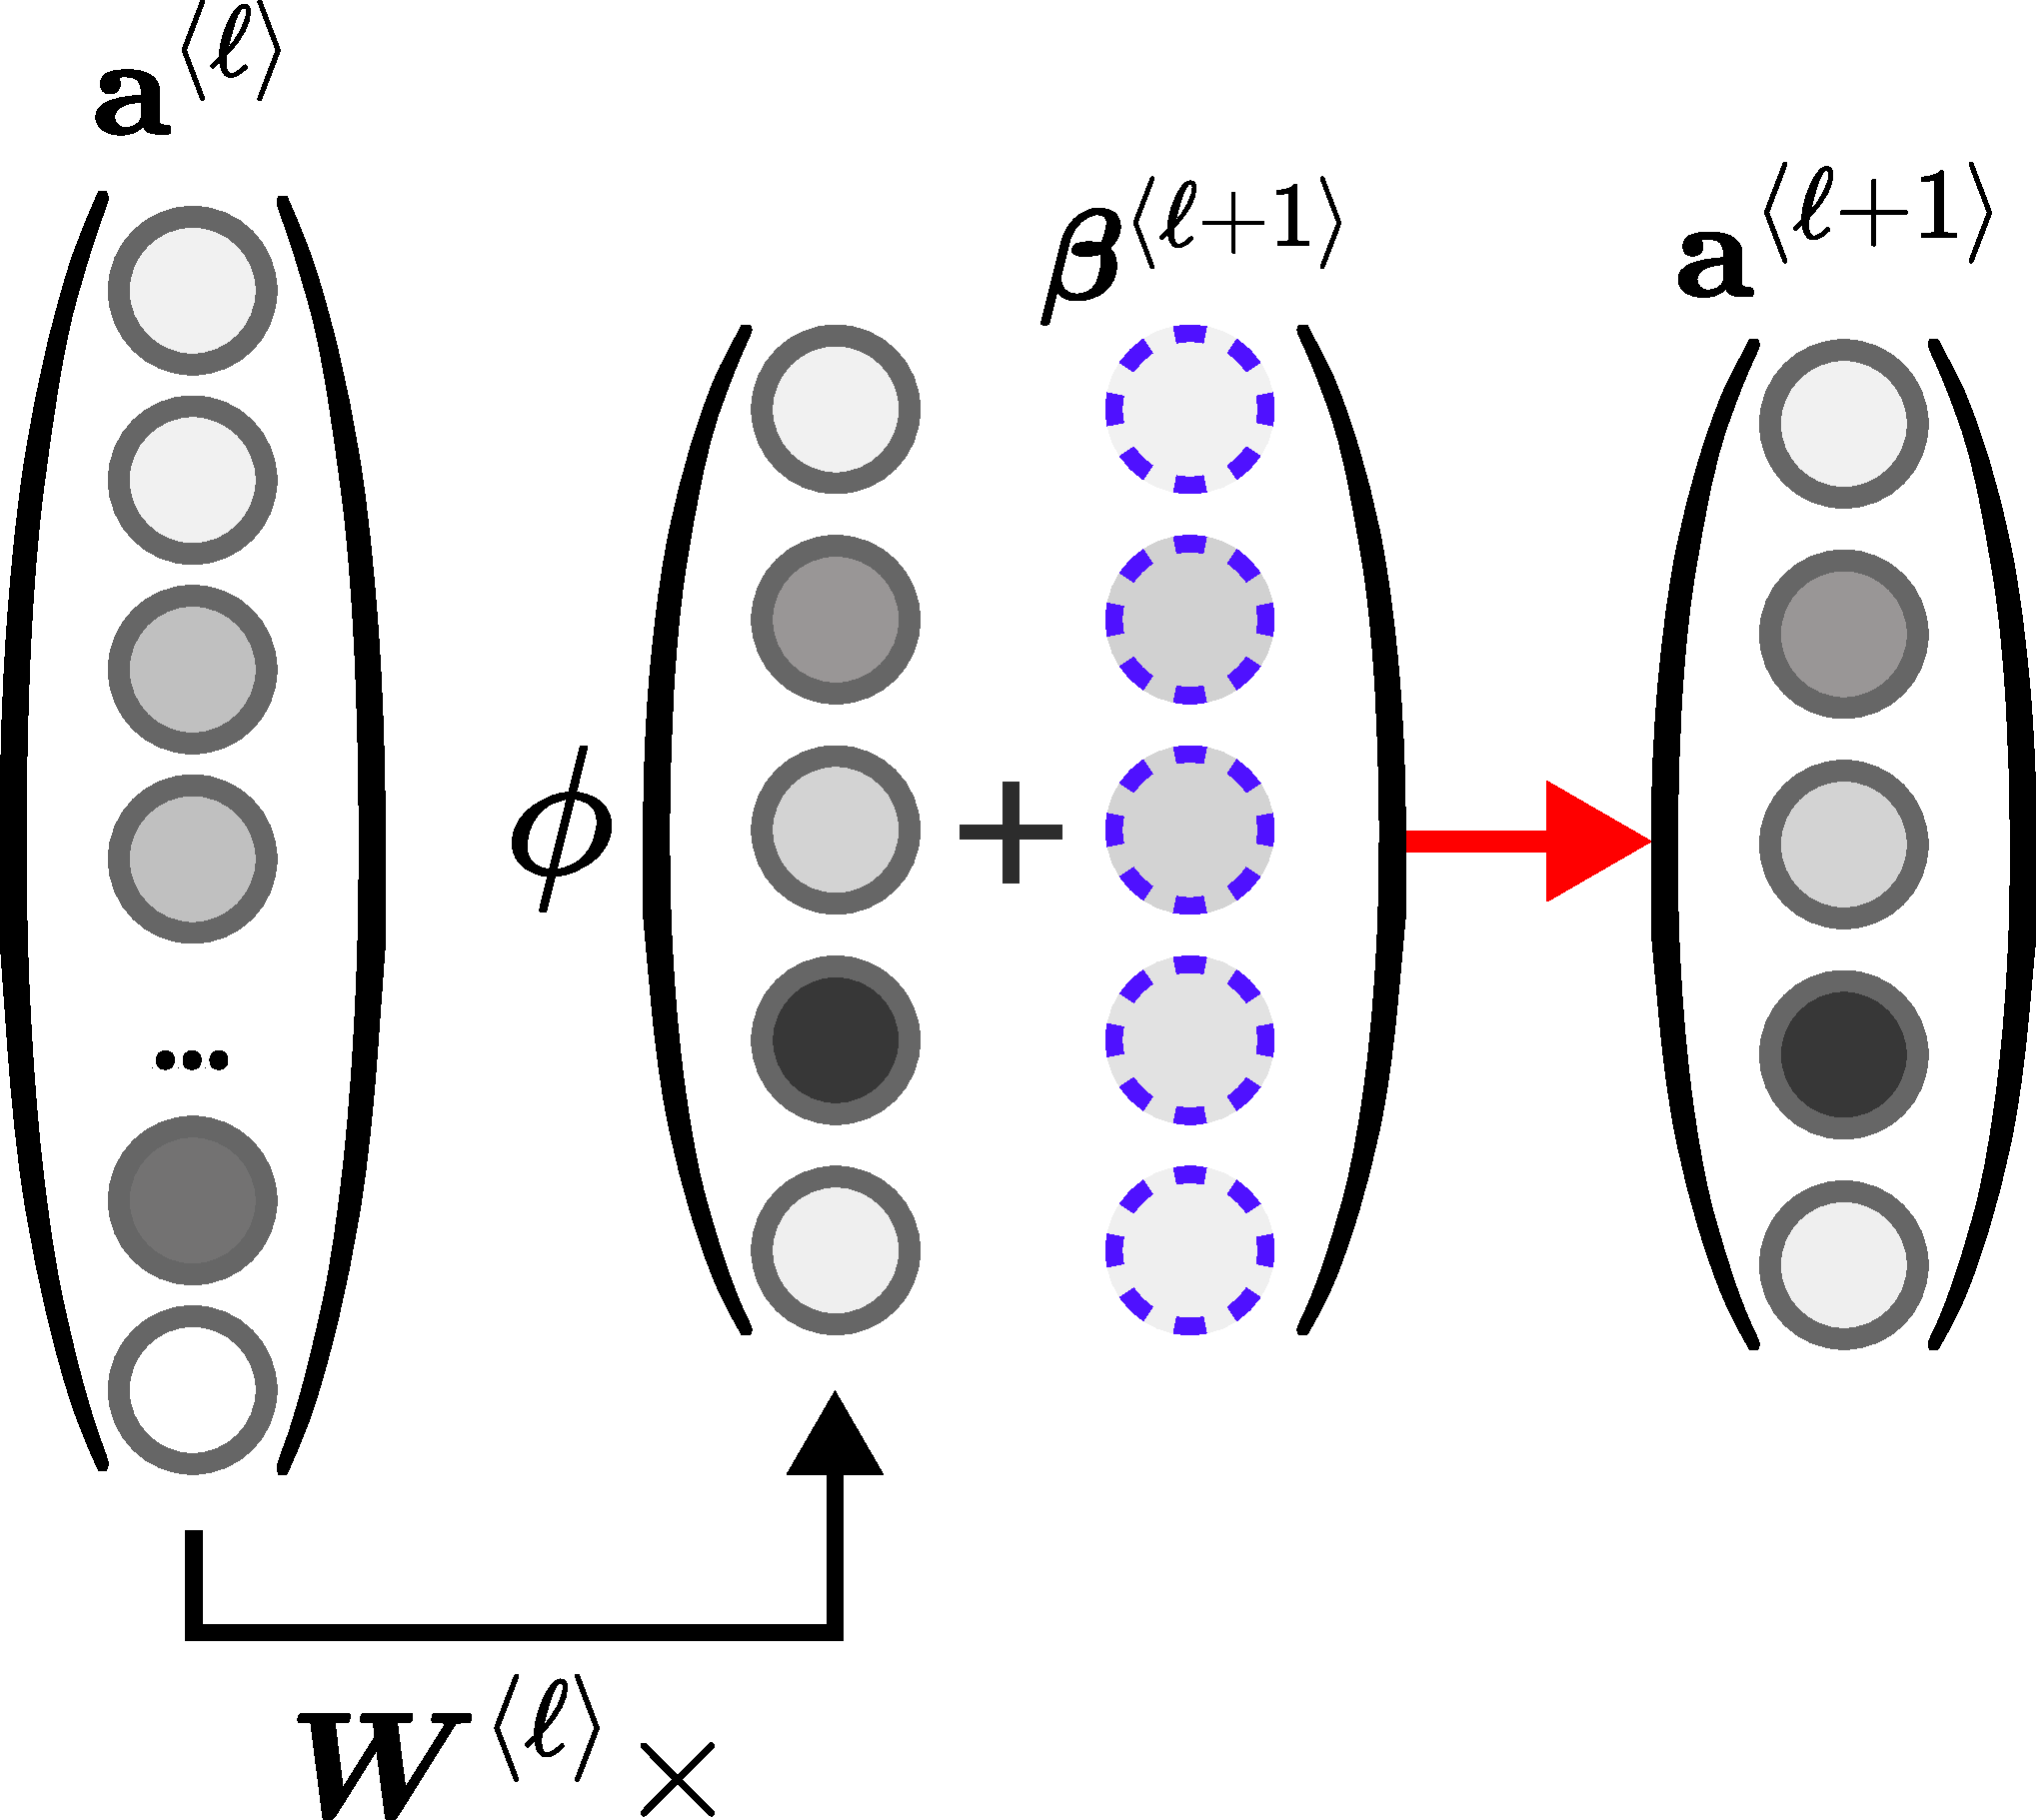
\includegraphics[width=\textwidth]{images/inference.pdf}
                    \end{figure}
                \end{column}
            
                \begin{column}{0.5\textwidth}
                    \textcolor{purple}{\textbf{Issue.}} Typically, after the linear operations, we
                    apply the non-linear operation (e.g., $\max\{0,x\}$). Each
                    one currently costs \textbf{255 constraints}. We have an
                    approach to reduce this cost down to $\approx 20$
                    constraints.
                \end{column}
            \end{columns}
        }
    \end{frame}

    \begin{frame}{Problems}
        \only<1-3>{
            \begin{itemize}[label=\cmark]
                \item \textbf{Problem 1.} Add support for more neural network layers.
                \item \textbf{Problem 2.} Activation-optimized neural networks are
                \textit{very hard} to train. Further optimizations allow more
                complex models $\implies$ better accuracy. E.g., 1 mln constraints
                $\approx$ 3900 non-linearities.
            \end{itemize}
        }

        \only<2>{
            \begin{figure}
                \centering
                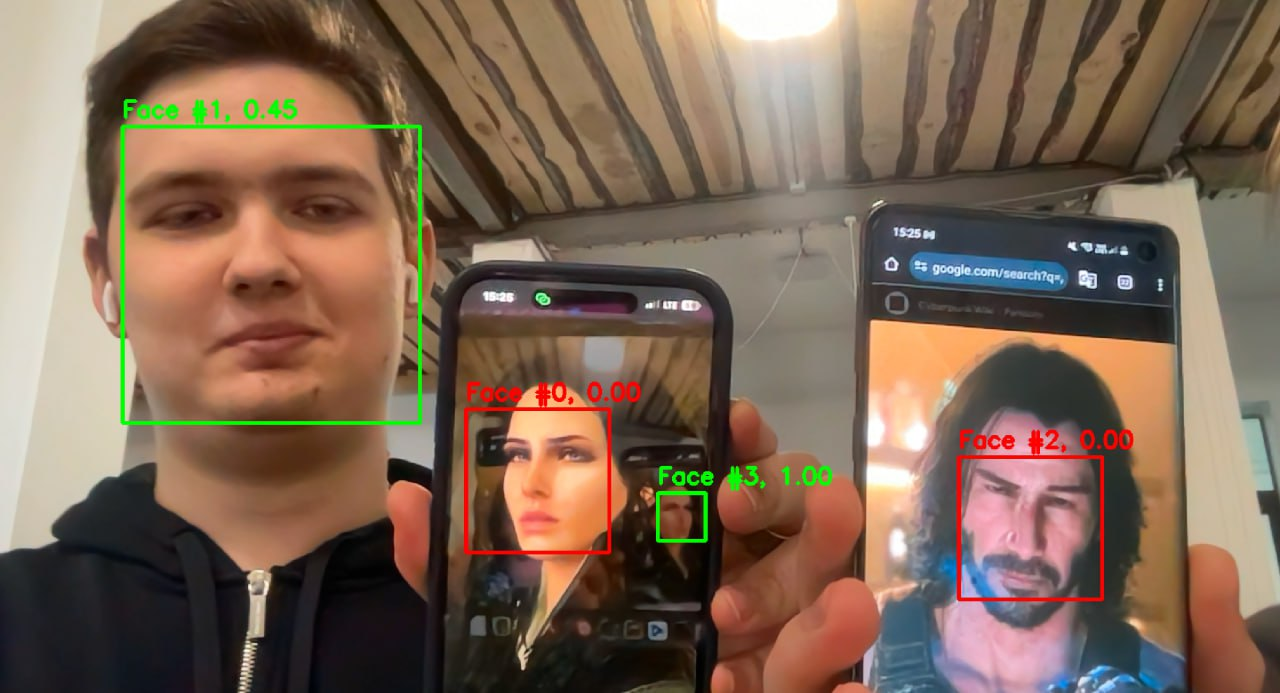
\includegraphics[width=0.8\textwidth]{images/problems_1.jpg}
                \caption{Shit happens}
            \end{figure}
        }
        \only<3>{
            \begin{figure}
                \centering
                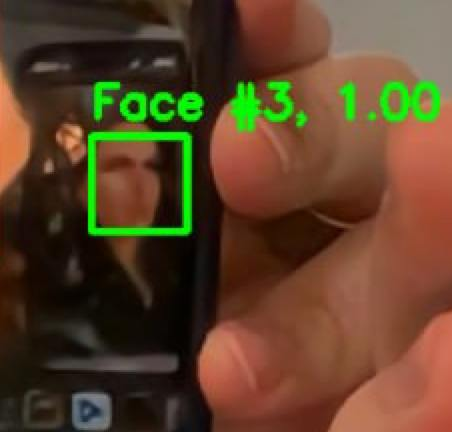
\includegraphics[width=0.45\textwidth]{images/problems_2.jpg}
            \end{figure}
        }
    \end{frame}

    \begin{frame}{Future Directions}
        \setlength{\fboxrule}{1.5pt}
            \fcolorbox{blue!70!black}{blue!10}{
                \parbox{0.9\linewidth}{
                    \textcolor{blue}{\textbf{Goal 1.}} Implement \textbf{UltraGroth}: $\approx 20$ gates per activation.
                }
            }

            \begin{figure}
                \centering
                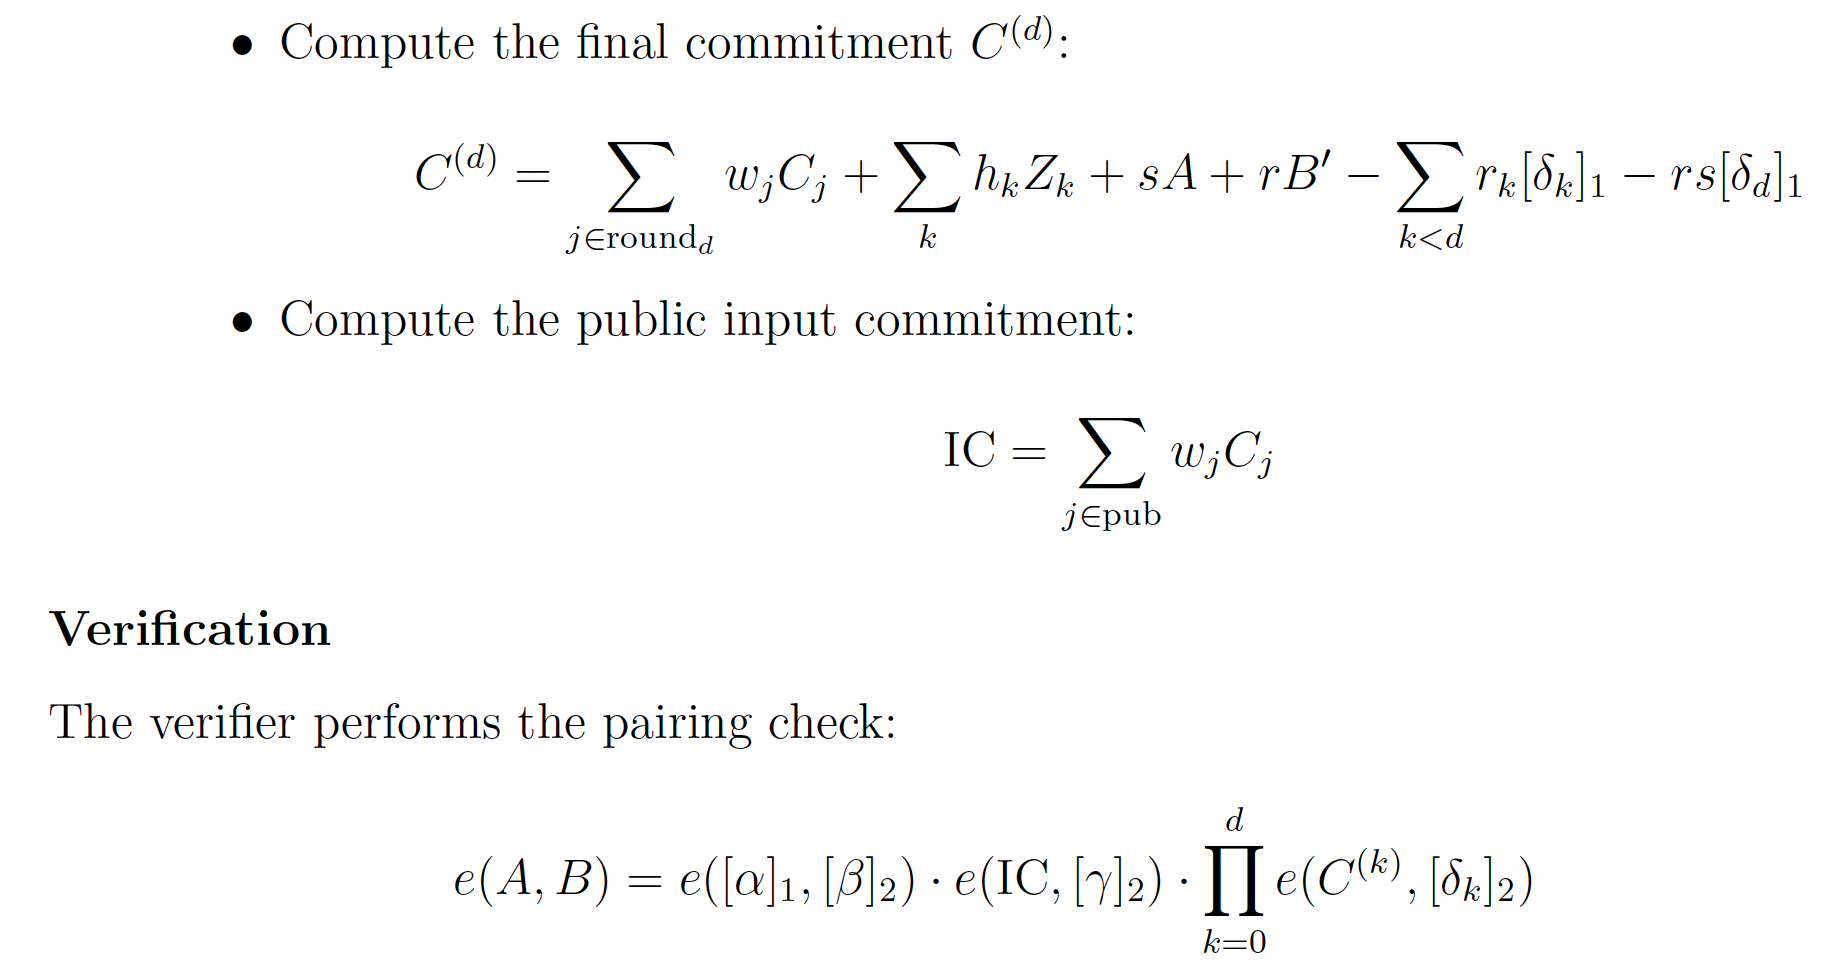
\includegraphics[width=0.8\textwidth]{images/ultragroth.png}
                \caption{Excerpt from our UltraGroth technical specification.}
            \end{figure}

            \begin{center}
                \textit{Can be used in other projects as well if you need effective range checks!}
            \end{center}
    \end{frame}

    \begin{frame}{Future Directions}
        \setlength{\fboxrule}{1.5pt}
            \fcolorbox{green!70!black}{green!10}{
                \parbox{0.9\linewidth}{
                    \textcolor{green!70!black}{\textbf{Goal 2.}} More blogs and media activity on the way.
                }
            }
            \begin{columns}
                \begin{column}{0.5\textwidth}
                    \begin{figure}
                        \centering
                        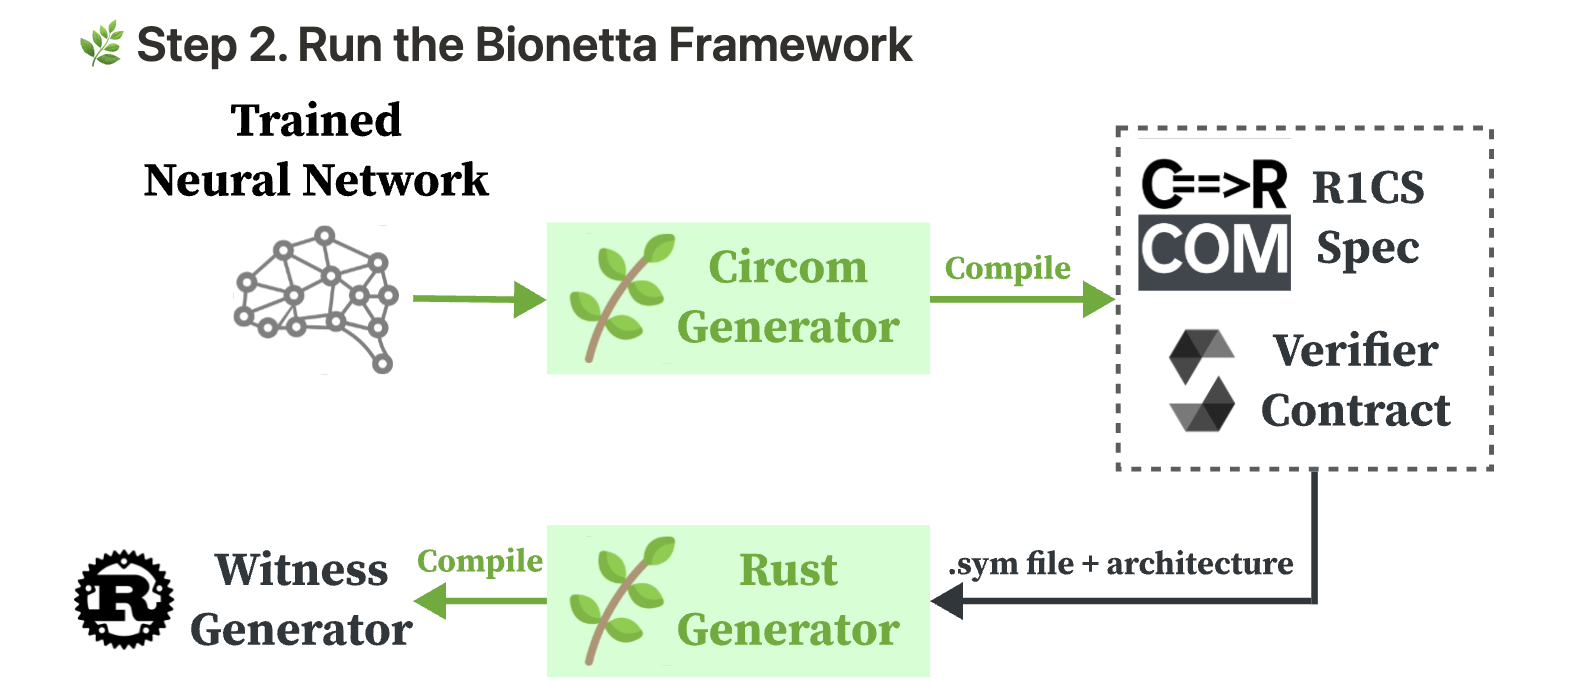
\includegraphics[width=0.8\textwidth]{images/media_enginnering_blog.png}
                        \caption{Engineering Blogs}
                    \end{figure}
                \end{column}
            
                \begin{column}{0.5\textwidth}
                    \begin{figure}
                        \centering
                        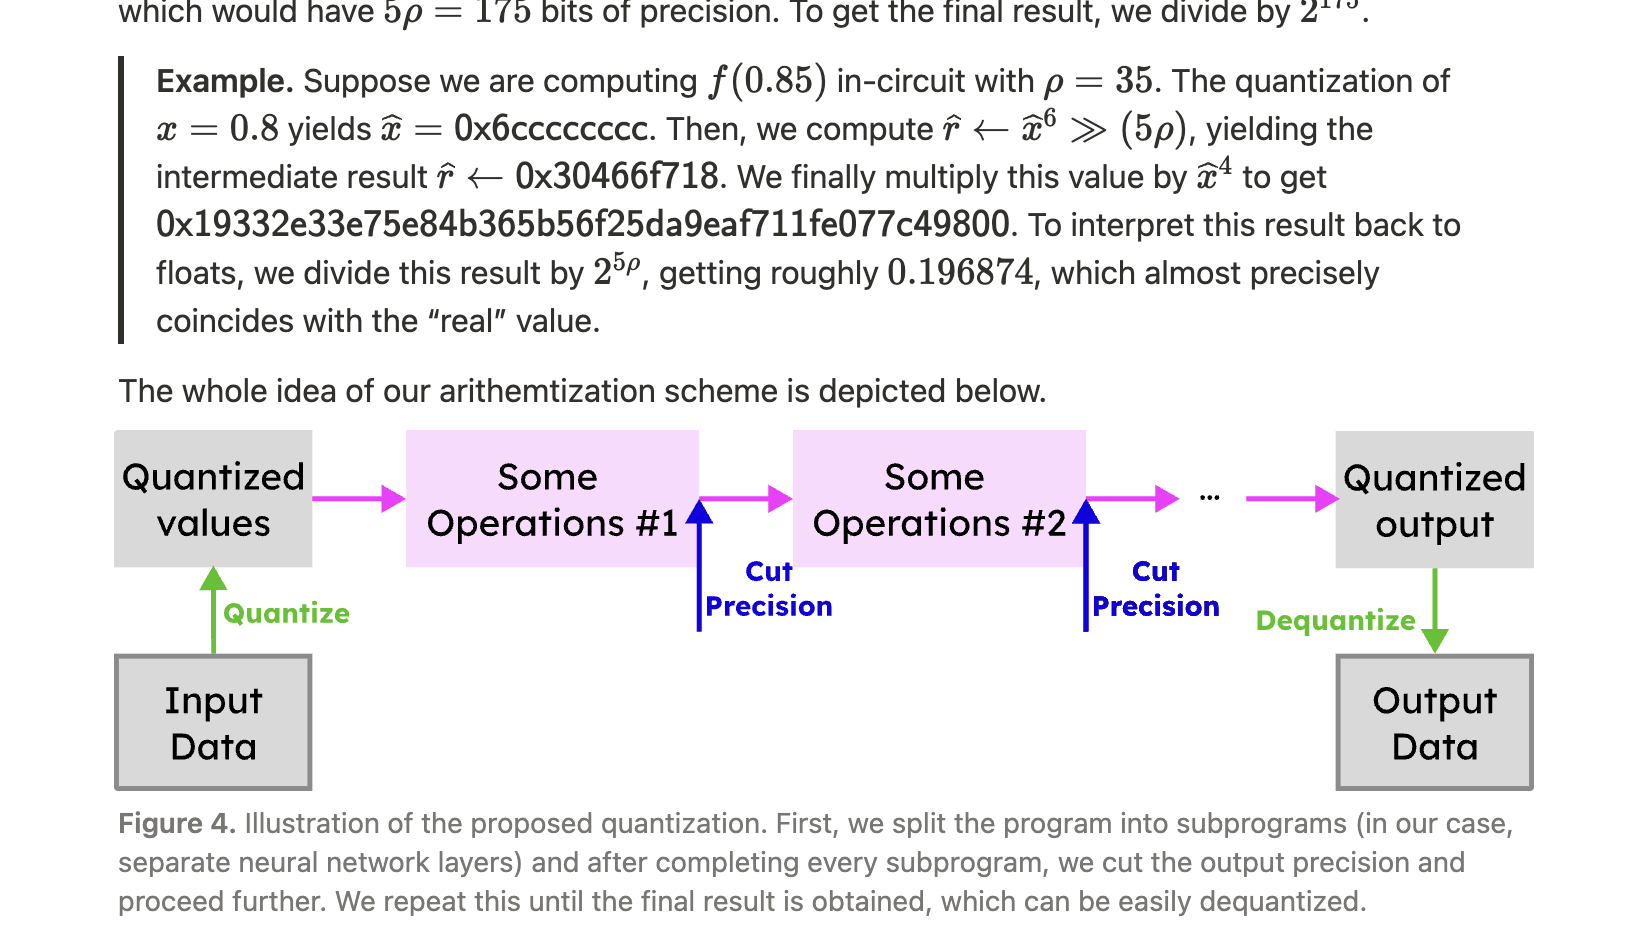
\includegraphics[width=0.8\textwidth]{images/media_tech_blog.png}
                        \caption{Technical Blogs}
                    \end{figure}
                \end{column}
            \end{columns}
            \begin{columns}
                \begin{column}{0.5\textwidth}
                    \begin{figure}
                        \centering
                        
\includegraphics[width=0.8\textwidth]{images/media_papers.png}
                        \caption{Research Papers}
                    \end{figure}
                \end{column}
                \begin{column}{0.5\textwidth}
                    \begin{figure}
                        \centering
                        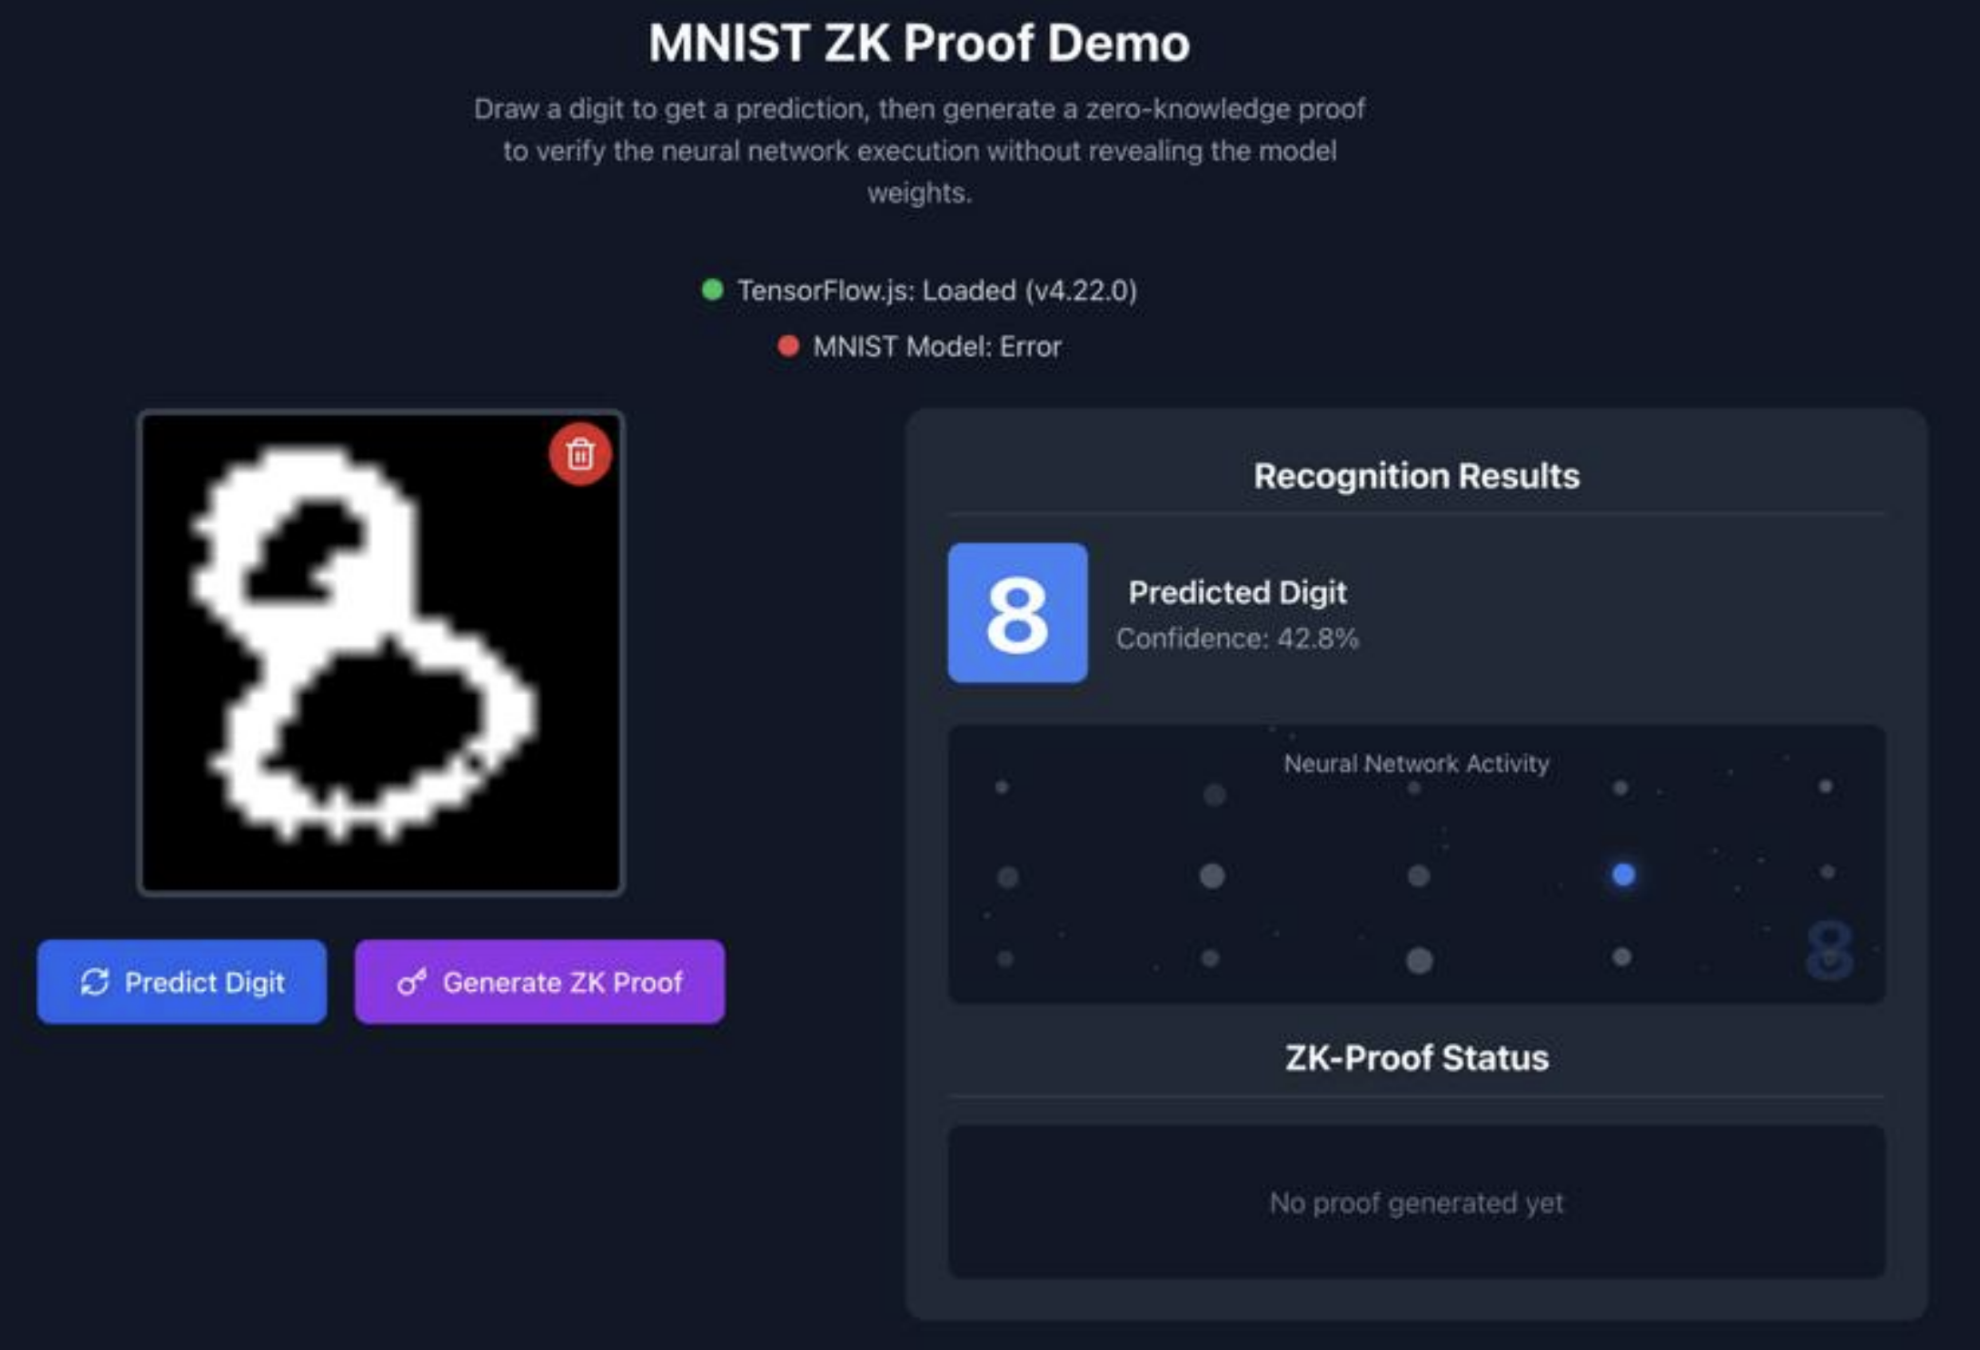
\includegraphics[width=0.8\textwidth]{images/media_demos.png}
                        \caption{Demos}
                    \end{figure}
                \end{column}
            \end{columns}
    \end{frame}

    \begin{frame}{Future Directions}
        \setlength{\fboxrule}{1.5pt}
            \fcolorbox{purple!70!black}{purple!10}{
                \parbox{0.9\linewidth}{
                    \textcolor{purple!70!black}{\textbf{Goal 3.}} Noir + Bionetta Integration.
                }
            }
            
            \begin{figure}
                \centering
                
\includegraphics[width=\textwidth]{images/bionetta_aztec.png}
            \end{figure}

            In particular, this includes:
            \begin{itemize}[label=\cmark]
                \item Custom ACIR to R1CS converter.
                \item Groth16 (\textcolor{gray}{\textit{and potentially UltraGroth}}) backend.
                \item Circuits written in a human-readable format (yes, Circom,
                we are looking at you).
            \end{itemize}
    \end{frame}

    \begin{frame}[plain, standout]
        \centering
        \LARGE
        \textbf{Any Questions?} \\
        
        \vspace{0.2cm} \Huge \ding{170} \large \\
        
        \vspace{1cm}
  
        \href{https://distributedlab.com/}{\raisebox{-.1em}{\hspace{.025em}\faIcon{globe}}\hspace{.325em}distributedlab.com} \\
  
        \href{https://github.com/rarimo/bionetta-tf}{\raisebox{-.1em}{\hspace{.025em}\faIcon{github}}\hspace{.325em}github.com/distributed-lab/nero}
        
        \begin{center}
            
\includegraphics[width=0.25\textwidth]{logo.png}
        \end{center}
    \end{frame}
\end{document}